\chapter{Mocny typ homotopijny}\label{chapter2}
\begin{center}
\begin{minipage}{14cm}
{\small
Mówimy, że przestrzeń topologiczna jest Aleksandrowa, o~ile przekrój każdej rodziny jej otwartych podzbiorów jest zbiorem otwartym. Przestrzenie $\mathrm{T_0}$~Aleksandrowa utożsamiać można z~częściowymi porządkami. \\

Korzystając z~pojęć rozbieralności oraz~rdzenia częściowego porządku dowodzimy, że dla dowolnej grupy $\Gamma$~dwie $\Gamma$-przestrzenie Aleksandrowa nie zawierające promieni (w~sensie teorioporządkowym) są $\Gamma$-homotopijnie równoważne wtedy i~tylko wtedy, gdy ich rdzenie są homeomorficzne.  Wykazujemy, że  nie istnieją nietrywialne H-przestrzenie oraz ko-H-przestrzenie Aleksandrowa bez promieni. Wprowadzamy pojęcia korozbieralności, lokalnej rozbieralności oraz s-ściągalności częściowych porządków i~dowodzimy ich własności. Część spośród tych rozważań przenosimy z~częściowych porządków na kompleksy symplicjalne oraz proponujemy definicję mocnego typu homotopijnego nieskończonego kompleksu symplicjalnego.\\

Rozdział opiera się częściowo na pracach autora \cite{Kukiela10a,Kukiela10} i~uogólnia ich wyniki, jak i~rezultaty uzyskane przez innych autorów \cite{Barmak12,Stong66,Stong84}.
}\end{minipage}\\[1.7cm]
\end{center}

Przestrzeń topologiczną $X$~nazywamy \textit{przestrzenią Aleksandrowa}\index{przestrzenzzz topologiczna@przestrzeń topologiczna!Aleksandrowa}, o~ile przekrój każdej rodziny otwartych podzbiorów $X$~jest zbiorem otwartym. Przestrzenie o~tej własności rozważane były w~latach 30-tych XX~wieku przez Aleksandrowa \cite{Alexandroff37} oraz Tuckera \cite{Tucker36}, a~także, w~nieco innym kontekście, przez Birkhoffa (zob.~\cite{Ronse}). Ważną podklasę przestrzeni Aleksandrowa tworzą skończone przestrzenie topologiczne. Kategoria przestrzeni Aleksandrowa i~ciągłych odwzorowań jest izomorficzna kategorii zbiorów quasi-uporządkowanych i~odwzorowań zachowujących porządek \cite{Alexandroff37,Tucker36}. Podobny fakt zachodzi dla kategorii przestrzeni Aleksandrowa spełniających aksjomat oddzielania $\mathrm{T_0}$~i~kategorii częściowych porządków.

Przestrzenie topologiczne Aleksandrowa odgrywają istotną rolę w~badaniach kraty wszystkich topologii na ustalonym zbiorze \cite{Steiner66,Watson94}, zob.~też \cite{Uzcategui05}. Długą tradycję mają wyniki dotyczące aproksymacji dowolnych przestrzeni topologicznych systemami odwrotnymi skończonych przestrzeni topologicznych (zob.~np.~\cite{Alexandroff47,Bandt92,Clader09,Flachsmeyer61,Kopperman05, Kopperman09,Shiraki76}, \cite[Chapter 49, Section 11]{Pearl07},\cite[p.~414]{Nagata85}). (Warto w~tym kontekście zwrócić uwagę na związek z~przestrzeniami spektralnymi, tj.~homeomorficznymi spektrum przemiennego pierścienia z~jedynką, które można scharakteryzować jako granice odwrotne systemów skończonych przestrzeni $\mathrm{T_0}$ \cite{Hochster69}.) Znalazły one zastosowania w~fizyce teoretycznej \cite{Sorkin91} oraz topologii cyfrowej \cite{Kopperman03,Kopperman05}, co wpłynęło w~ostatnich latach na wzrost zainteresowania skończonymi przestrzeniami topologicznymi. Przestrzenie Aleksandrowa, jako obiekty o~wyjątkowych własnościach i~stosunkowo prostej strukturze, dostarczać mogą ponadto kontrprzykładów, czy też stanowić pole do testowania ogólnych hipotez (por.~\cite{Kukiela09,Kukiela13a,Barmak}), a~także służyć jako narzędzie pedagogiczne \cite{Helmstutler12,May}.

W~niniejszej rozprawie na przestrzenie Aleksandrowa patrzymy od strony topologii algebraicznej. Podejście to zainicjowane zostało dwoma artykułami z~1966 roku, autorstwa McCorda \cite{McCord66} oraz Stonga \cite{Stong66}. 

McCord \cite{McCord66} dowiódł, iż każdy kompleks symplicjalny $K$~ma słaby typ homotopijny przestrzeni Aleksandrowa odpowiadającej częściowemu porządkowi $\mP(K)$~stowarzyszonemu z~tym kompleksem; odwrotnie, każda przestrzeń Aleksandrowa $X$~jest słabo homotopijnie równoważna kompleksowi symplicjalnemu $\mK(X)$~stowarzyszonemu z~tą przestrzenią (traktowaną jako częściowy porządek). Przykładowo, dla każdej liczby naturalnej $n$~istnieje słabo homotopijnie równoważna $n$-wymiarowej sferze $\S^n$ skończona przestrzeń topologiczna o~$2n+2$ elementach (por.~\cite[Theorem 2.13]{Barmak07}). 

Praca Stonga \cite{Stong66} dotyczyła natomiast typu homotopijnego skończonych przestrzeni topologicznych, który bardzo różni się od ich słabego typu homotopijnego: nietrudno np.~zauważyć, że każda spójna przestrzeń $\mathrm{T_1}$~mająca typ homotopijny przestrzeni Aleksandrowa jest ściągalna, co wyraźnie kontrastuje wynikami McCorda. Stong \cite{Stong66} podał między innymi pewnego rodzaju klasyfikację typów homotopijnych skończonych przestrzeni topologicznych: każdą taką przestrzeń można sprowadzić do tzw.~rdzenia (będącego jej retraktem o~specjalnych własnościach), przy czym dwie skończone przestrzenie są homotopijnie równoważne dokładnie wtedy, gdy ich rdzenie są homeomorficzne. Wykorzystał w~tym celu dobrze znane i~szeroko stosowane również w~innych kontekstach pojęcie rozbieralności częściowego porządku (krótki przegląd związanej z~nim literatury znajduje się w~sekcji \ref{subsec-rdzenie_i_rozb_p_Al}).

Wydaje się, że po roku 1966~przez wiele lat temat topologii algebraicznej przestrzeni Aleksandrowa nie wzbudzał większego zainteresowania, choć w~1969 ukazał się (mało znany) artykuł autorstwa Shiraki \cite{Shiraki69}, zaś w~1978 ważna praca Quillena \cite{Quillen78}, którą w~1984 Stong \cite{Stong84} powiązał z~wcześniejszymi rozważaniami swoimi \cite{Stong66} oraz McCorda \cite{McCord66}.  Dopiero w~latach \mbox{90-tych} temat ten zaczął ponownie zajmować badaczy, a~po roku 2000 liczba publikowanych prac dotyczących teorii homotopii przestrzeni skończonych i~Aleksandrowa wzrosła bardzo dynamicznie (przegląd niektórych spośród nich znajduje się w~sekcji \ref{subsec-tw_mccorda_i_stonga}). Wśród nich ukazał się artykuł Arenasa \cite{Arenas99}, jednym z~celów którego było uogólnienie wyników Stonga dotyczących typu homotopijnego skończonych przestrzeni topologicznych na lokalnie skończone przestrzenie Aleksandrowa. Autor rozprawy zauważył błąd w~pracy Arenasa, a~próby jego poprawienia zaowocowały powstaniem artykułu \cite{Kukiela10a} oraz pracy magisterskiej \cite{Kukiela10}, w~których wyniki Stonga uogólnia się na pewną klasę nieskończonych przestrzeni Aleksandrowa, zawartą w~klasie przestrzeni Aleksandrowa bez promieni. (Przez przestrzeń Aleksandrowa bez promieni rozumiemy taką przestrzeń Aleksandrowa, że odpowiadający jej częściowy porządek nie zawiera promieni.)

Głównym wynikiem bieżącego rodziału jest twierdzenie \ref{wniosek_klasyfikacyjny}, rozszerzające klasyfikację typów homotopijnych Stonga \cite{Stong66} na wszystkie przestrzenie Aleksandrowa bez promieni; stanowi ono uogólnienie wcześniejszych wyników autora \cite{Kukiela10,Kukiela10a}. Interesujące wnioski z~tego twierdzenia dotyczą nieistnienia nietrywialnych H-przestrzeni (stwierdzenia \ref{stw-stonga_o_h_przestrzeniach}) oraz~ko-H-przestrzeni (stwierdzenie \ref{stw-helmsutlera-vaughna}) Aleksandrowa bez promieni; wzorują się one na analogicznych wynikach Stonga \cite{Stong66}, Helmstutlera i~Vaughna \cite{Helmstutler10}. W~rozważaniach wykorzystujemy pojęcie rozbieralności częściowego porządku. Ze~względu na zastosowania w~dalszej części rozprawy definiujemy związane z~nim: korozbieralność, lokalną rozbieralność oraz~s-ściągalność, i~dowodzimy niektórych ich własności. Szczególnie ciekawe jest twierdzenie \ref{build_if_dism}, mówiące że w~przypadku częściowych porządków bez promieni pojęcia rozbieralności oraz korozbieralności są równoważne. Rozdział kończy się wynikami dotyczącymi kompleksów symplicjalnych. Formułujemy (wzorując się na pracy Barmaka i~Miniana \cite{Barmak12}) definicje (ko)rozbieralności oraz mocnego typu homotopijnego kompleksu symplicjalnego i~dowodzimy związków tych pojęć z~(ko)rozbieralnością oraz typem homotopijnym stowarzyszonych przestrzeni Aleksandrowa. Znaczna część wyników rozdziału jest wykorzystywana w~dalszej części rozprawy.

Rozdział zorganizowany jest w~następujący sposób. W~podrozdziale \ref{sec-top_ogol_p_aleks} przywołujemy niektóre fakty z~zakresu topologii ogólnej przestrzeni Aleksandrowa. Podrozdział \ref{sec-typy_hom_p_aleks} dotyczy typu homotopijnego przestrzeni Aleksandrowa. Rozpoczynamy go od omówienia wyników prac McCorda \cite{McCord66} i~Stonga \cite{Stong66}. Przypominamy pojęcie rozbieralności i~rdzenia nieskończonej przestrzeni Aleksandrowa, a~także definiujemy korozbieralność i~dowodzimy jej własności. Następnie podajemy twierdzenie ,,klasyfikujące'' typy homotopijne przestrzeni Aleksandrowa bez promieni i~wyciągamy wnioski dotyczące (ko)-H-przestrzeni Aleksandrowa. Podrozdział \ref{sec-mocny_typ_homotopijny} poświęcony jest rozbieralności i~korozbieralności kompleksów symplicjalnych oraz ich mocnemu typowi homotopijnemu.

%==============================================================
%==============================================================
%==============================================================

\section{Topologia ogólna przestrzeni Aleksandrowa}\label{sec-top_ogol_p_aleks}
Niniejszy podrozdział przybliża niektóre fakty~z~zakresu topologii ogólnej przestrzeni Aleksandrowa. Rozpoczynamy od przedstawienia ścisłego związku tych przestrzeni z~częściowymi porządkami, znanego już w~latach \mbox{30-tych} XX~wieku \cite{Alexandroff37,Tucker36,Ronse}. Następnie podajemy wyniki związane ze zwartością, spójnością oraz topologią przestrzeni funkcji ciągłych pomiędzy przestrzeniami Aleksandrowa. Część z~nich przenosi się natychmiast z~przypadku skończonych przestrzeni topologicznych (por.~\cite{May08,Stong66}),  pozostałe cytujemy z~prac autora \cite{Kukiela10a,Kukiela10}.


%---------------------------------------------------------------
%---------------------------------------------------------------
%---------------------------------------------------------------


\subsection{Związek z~częściowymi porządkami}
Niech $(X,\tau)$~będzie przestrzenią topologiczną. \textit{Quasi-porządkiem specjalizacji}\index{quasi-porzazzzdek@quasi-porządek!specjalizacji}\index{quasi-porzazzzdek@quasi-porządek!stowarzyszony z~przestrzeniazzz topologicznazzz@stowarzyszony z przestrzenią topologiczną}\index{czezzzszzzciowy porzazzzdek@częściowy porządek!specjalizacji}\index{czezzzszzzciowy porzazzzdek@częściowy porządek!stowarzyszony z!t0 przestrzeniazzz topologicznazzz@$\mathrm{T_0}$ przestrzenią topologiczną} na $X$~nazywamy relację $\leq_\tau\subseteq X\times X$ taką, że $x\leq_\tau y$, gdy $y\in \overline{\{x\}}$. (Część autorów za quasi-porządek specjalizacji przyjmuje quasi-porządek dualny do wyżej zdefiniowanego.) Przyjmijmy oznaczenie $\mO(X)=(X,\leq_\tau)$. Dla ciągłego odwzorowania $f\colon X\to Y$ przez $\mO(f)\colon \mO(X)\to \mO(Y)$ oznaczamy zachowujące quasi-porządek odwzorowanie o~tym samym co $f$~wykresie. Przyporządkowanie $\mO\colon \mathbf{\mathbf{T}op}\to \mathbf{\mathbf{Q}uoset}$\nomenclature[6d]{$\mO$}{funktor quasi-porządku specjalizacji} z~kategorii przestrzeni topologicznych i~ciągłych odwzorowań w~kategorię quasi-porządków i~przekształceń zachowujących quasi-porządek jest funktorem.

Nietrudno zauważyć, że $X$~jest przestrzenią $\mathrm{T_0}$ wtedy i~tylko wtedy, gdy $\mO(X)$ jest częściowym porządkiem. Ponadto $X$~spełnia aksjomat $\mathrm{T_1}$~dokładnie wtedy, gdy $\mO(X)$~jest antyłańcuchem.

Niech $(P,\leq)$ będzie zbiorem quasi-uporządkowanym. Przez $\mX(P)=(P,\tau_\leq)$\index{przestrzenzzz topologiczna@przestrzeń topologiczna!Aleksandrowa!stowarzyszona z quasi-porzazzzdkiem@stowarzyszona z quasi-porządkiem} oznaczamy przestrzeń topologiczną taką, że $\tau_\leq$ jest topologią na $P$~generowaną przez bazę zbiorów otwartych $\{p\mathord{\downarrow}\}_{p\in P}$. Jak łatwo spostrzec, $\mX(P)$ jest przestrzenią Aleksandrowa. Ponadto $P$~jest częściowym wtedy i~tylko wtedy, gdy $\mX(P)$ jest przestrzenią $\mathrm{T_0}$. Dla zachowującego quasi-porządek odwzorowania $f\colon P\to Q$ przez $\mX(f)\colon \mX(P)\to \mX(Q)$ oznaczamy ciągłe odwzorowanie o~tym samym co $f$~wykresie. Przyporządkowanie $\mX\colon \mathbf{\mathbf{Q}uoset}\to \mathbf{\mathbf{A}l}$\nomenclature[6f]{$\mX$}{funktor przestrzeni topologicznej Aleksandrowa stowarzyszonej z~quasi-porządkiem} z~kategorii quasi-porządków i~przekształceń zachowujących quasi-porządek w~kategorię przestrzeni Aleksandrowa i~ich ciągłych odwzorowań jest funktorem.

Oznaczmy przez 
\begin{align*}
&\mO\big|_{\mathbf{\mathbf{A}l}}\colon \mathbf{\mathbf{A}l}\to \mathbf{\mathbf{Q}uoset},\\
&\mO\big|_{\mathbf{T_0\mathbf{A}l}}\colon \mathbf{T_0\mathbf{A}l}\to \mathbf{\mathbf{P}oset},\\
&\mX\big|_{\mathbf{\mathbf{P}oset}}\colon \mathbf{\mathbf{P}oset}\to \mathbf{T_0\mathbf{A}l}
\end{align*}
odpowiednie ograniczenia rozważanych funktorów ($\mathbf{T_0\mathbf{A}l}$~oznacza kategorię $\mathrm{T_0}$~przestrzeni Aleksandrowa, zaś $\mathbf{\mathbf{P}oset}$ kategorię częściowych porządków). Okazuje się, że \[\mO\big|_{\mathbf{\mathbf{A}l}}\circ \mX=\id_{\mathbf{\mathbf{Q}uoset}},\quad \mX\circ \mO\big|_{\mathbf{\mathbf{A}l}}=\id_{\mathbf{\mathbf{A}l}}\] oraz \[\mO\big|_{\mathbf{T_0\mathbf{A}l}}\circ \mX\big|_{\mathbf{\mathbf{P}oset}}=\id_{\mathbf{\mathbf{P}oset}},\quad \mX\big|_{\mathbf{\mathbf{P}oset}}\circ \mO\big|_{\mathbf{T_0\mathbf{A}l}}=\id_{\mathbf{T_0\mathbf{A}l}},\]
co oznacza, że kategorie $\mathbf{\mathbf{Q}uoset}$ oraz $\mathbf{\mathbf{A}l}$ są izomorficzne, podobnie jak kategorie $\mathbf{\mathbf{P}oset}$, $\mathbf{T_0\mathbf{A}l}$. Ponadto, jak nietrudno zauważyć, podprzestrzenie przestrzeni Aleksandrowa odpowiadają przy tym izomorfizmie podzbiorom quasi-uporządkowanym ich quasi-porządków specjalizacji. Innymi słowy, jeśli $(X,\tau)\in\mathbf{Al}$ oraz $A\subseteq X$, to topologia indukowana na $A$~pokrywa się z~topologią przestrzeni $\mX\left(\big(A,\leq_\tau\!\big|_{A}\big)\right)$.\\

\textbf{Przy rozważaniu przestrzeni Aleksandrowa pomijać będziemy odtąd na ogół w~zapisach funktory $\mO,\mX$, utożsamiając zbiory quasi-uporządkowane i~odwzorowania zachowujące quasi-porządek z~odpowiadającymi im przestrzeniami Aleksandrowa i~odwzorowaniami ciągłymi.}\\

Zastosowanie języka quasi-porządków pozwoli w~wygodny sposób opisać wiele topologicznych własności przestrzeni Aleksandrowa. 

Przyjmijmy jeszcze jedno techniczne założenie, które pozwoli znacząco uprościć zapisy.\\

\textbf{Do końca rozdziału wszystkie rozważane przestrzenie topologiczne spełniają aksjomat oddzielania $\mathrm{T_0}$.}\\

Ograniczenie się do przestrzeni $\mathrm{T_0}$~nie zuboży w~istotny sposób prowadzonych rozważań, gdyż każda przestrzeń topologiczna jest homotopijnie równoważna swojej (spełniającej aksjomat $\mathrm{T_0}$) przestrzeni ilorazowej powstałej przez utożsamienie punktów nie rozróżnianych przez topologię (por.~np.~\cite[podrozdział I.4]{Kukiela10}).

Informacje o~innych związkach topologii i~teorii porządku, w~podobnym duchu do przedstawionych w~tej sekcji, odnaleźć można w~pracy Ern{\'e} \cite{Erne90}.


%---------------------------------------------------------------
%---------------------------------------------------------------
%---------------------------------------------------------------


\subsection{Spójność, zwartość, przestrzenie funkcyjne}
Przypomnimy wyniki związane z~pojęciami spójności i~zwartości w~przestrzeniach Aleksandrowa, a~także z~topologią zwarto-otwartą na przestrzeni funkcji ciągłych pomiędzy dwiema przestrzeniami Aleksandrowa. Część z~nich jest klasyczna, niektóre natomiast pochodzą z~prac autora \cite{Kukiela10a,Kukiela10}.

Zauważmy, że porównywalne (w~porządku specjalizacji) elementy przestrzeni Aleksandrowa można połączyć drogą.
\begin{stw}[{\cite{Stong66}}]\label{stw-droga_miedzy_porownywalnymi}
Niech $X$~będzie przestrzenią Aleksandrowa oraz niech $x,y\in X$ będą takie, że $x\leq y$. Wówczas odwzorowanie $h\colon \I\to X$ zadane dla $t\in \I$ wzorem \[h(t)=\begin{cases}x & \text{dla } t\in [0,1),\\ y & \text{dla } t=1\end{cases}\] jest ciągłe.
\end{stw}
Zbiory otwarte $\{x\mathord{\downarrow}\}$ są zatem łukowo spójne. Ponieważ tworzą one bazę otwartą topologii przestrzeni $X$, otrzymujemy następujący wniosek.
\begin{wn}[{\cite{Stong66}}]
Przestrzenie Aleksandrowa są lokalnie łukowo spójne.
\end{wn}
Nietrudno opisać składowe spójności przestrzeni Aleksandrowa.
\begin{wn}[{\cite{Stong66}}]\label{wn-stonga_o_skl_spojnosci}
Niech $X$~będzie przestrzenią Aleksandrowa. Składową spójności punktu $x\in X$ (równą składowej łukowej spójności tego punktu) jest zbiór \[\{y\in X: \text{istnieje ścieżka prosta w } \Comp(X) \text{ prowadząca z } x \text{ do } y\}.\]
\end{wn}
Łatwo też podać charakteryzację zwartych przestrzeni Aleksandrowa (przypomnijmy, że w~definicji zwartości nie zakładamy aksjomatu oddzielania $\mathrm{T_2}$). 
\begin{stw}[{\cite[Proposition 3.2]{Kukiela10a},\cite[stwierdzenie II.3.1]{Kukiela10}}]
Przestrzeń Aleksandrowa $X$~jest zwarta wtedy i~tylko wtedy, gdy zbiór $\max(X)$ jest skończony oraz dla każdego $y\in X$ istnieje $x\in\max(X)$ takie, że $x\geqslant y$.
\end{stw}

Przestrzeń topologiczną nazywamy \textit{dziedzicznie zwartą}\index{przestrzenzzz topologiczna@przestrzeń topologiczna!dziedzicznie zwarta}, gdy każda jej podprzestrzeń jest zwarta.

\begin{stw}[{\cite[Proposition 3.3]{Kukiela10a},\cite[stwierdzenie II.3.2]{Kukiela10}}]
Przestrzeń Aleksandrowa $X$ jest dziedzicznie zwarta wtedy i~tylko wtedy, gdy porządek dualny do $X$~jest dobrze ufundowany i~nie zawiera nieskończonych antyłańcuchów.
\end{stw}

(Dobrze ufundowane częściowe porządki nie zawierające nieskończonych antyłańcuchów nazywa się \textit{zbiorami częściwo dobrze uporządkowanymi}. Były one ,,odkrywane'' niezależnie przez wielu autorów, w~różnych kontekstach, por.~\cite{Kruskal72}.)

Przypomnijmy, że dla przestrzeni topologicznych $X$, $Y$~oraz ich podzbiorów $A\subseteq X$, $B\subseteq Y$ symbolem $[A,B]$ oznaczamy zbiór tych ciągłych funkcji $f\colon X\to Y$, które spełniają warunek $f(A)\subseteq B$.

\begin{stw}[{\cite[Corollary 3.4]{Kukiela10a},\cite[stwierdzenie II.4.2]{Kukiela10}}]
Niech $X, Y$~będą przestrzeniami Aleksandrowa. Rodzina $\left\{[x,y\mathord{\downarrow}]:x\in X,y\in Y\right\}$ stanowi wówczas podbazę otwartą topologii zwarto-otwartej na $\Cont(X,Y)$. Topologia zwarto-otwarta na $\Cont(X,Y)$ pokrywa się zatem z~topologią indukowaną przez topologię Tichonowa na podprzestrzeni $\Cont(X,Y)\subseteq \prod_{x\in X}Y$.
\end{stw}

\begin{stw}[{\cite[p.~12]{Kukiela10a},\cite[stwierdzenie II.4.1]{Kukiela10}}]\label{stw-porzadek_na_cxy}
Niech $X,Y$ będą przestrzeniami Aleksandrowa. Wówczas w~zbiorze uporządkowanym $\mO(C(X,Y))$ nierówność $f\leq g$ zachodzi dla $f,g\in \Cont(X,Y)$ wtedy i~tylko wtedy, gdy $f(x)\leq g(x)$ dla wszystkich $x\in X$.
\end{stw}

Nasuwa się pytanie, czy przestrzeń $\Cont(X,Y)$, gdzie $X,Y$ są przestrzeniami Aleksandrowa, jest również Aleksandrowa. Jeśli przestrzenie $X,Y$ są skończone, jest to oczywiście prawdą (gdyż wówczas przestrzeń $\Cont(X,Y)$ jest również skończona). Zgodnie ze sformułowanym niżej twierdzeniem, stanowiącym jeden z~głównych wyników pracy magisterskiej autora \cite{Kukiela10}, w~ogólności nie musi tak jednak być. Przeoczenie tego faktu stanowi podłoże wspomnianych we wstępie do rozdziału błędów w~pracy Arenasa \cite{Arenas99}.
\begin{tw}[{\cite[Corollary 3.5]{Kukiela10a},\cite[stwierdzenie II.4.2]{Kukiela10}}]\label{tw-kukiely-kiedy_cxy_aleksandrowa}
Niech $X,Y$~będą przestrzeniami Aleksandrowa oraz niech $Y$~zawiera co najmniej dwa elementy. Wówczas:
\begin{compactitem}
\item[---] jeśli przestrzeń $Y$~jest dyskretna, to $\Cont(X,Y)$ jest przestrzenią Aleksandrowa wtedy i~tylko wtedy, gdy liczba składowych spójności przestrzeni $X$~jest skończona;
\item[---] jeśli przestrzeń $Y$~nie jest dyskretna, to $\Cont(X,Y)$ jest przestrzenią Aleksandrowa wtedy i~tylko wtedy, gdy przestrzeń $X$~jest dziedzicznie zwarta oraz dla każdej funkcji $f\in \Cont(X,Y)$ zbiór $f(X)\subseteq Y$ jest skończony. 
\end{compactitem}
\end{tw}
\begin{wn}[{\cite[Corollary 3.6]{Kukiela10a},\cite[wniosek II.4.7]{Kukiela10}}]
Jeśli $X$~jest nieskończoną przestrzenią Aleksandrowa, to $\Cont(X,X)$ nie jest przestrzenią Aleksandrowa.
\end{wn}

Przy badaniu przestrzeni Aleksandrowa z~punktu widzenia teorii homotopii użyteczny jest następujący lemat Foxa \cite{Fox45}.

\begin{lem}[{\cite[Theorem 2]{Fox45}}]
Niech $X,T$ będą przestrzeniami topologicznymi spełniającymi pierwszy aksjomat przeliczalności. Wówczas dla dowolnej przestrzeni topologicznej $Y$~ciągłość odwzorowania $h:X\times T\to Y$ jest równoważna ciągłości funkcji $h^{*}:T\to \Cont(X,Y)$ zadanej dla $t\in T$ oraz $x\in X$ wzorem $h^*(t)(x)=h(x,t)$.
\end{lem}

Każda przestrzeń Aleksandrowa spełnia pierwszy aksjomat przeliczalności, gdyż dowolny jej element $x$~ma jednoelementową bazę otoczeń otwartych $\{x\mathord{\downarrow}\}$. Jeśli zatem w~powyższym lemacie za $X$~przyjmiemy przestrzeń Aleksandrowa, zaś za $T$~odcinek jednostkowy $\I$, otrzymamy poniższy wniosek, pozwalający na utożsamianie homotopii z~drogami w~przestrzeni odwzorowań (i~stanowiący odpowiedź na pytanie Lawsona \cite[p.~837]{Rival82}).

\begin{wn}\label{wn-homotopia_to_droga}
Niech $X$~będzie przestrzenią Aleksandrowa. Dla dowolnej przestrzeni topologicznej $Y$~ciągłość homotopii $h:X\times \I\to Y$ jest równoważna ciągłości odwzorowania $h^*:\I\to C(X,Y)$ zadanego dla $t\in\I$ oraz $x\in X$ wzorem $h^*(t)(x)=h(x,t)$.
\end{wn}

Z~wniosku \ref{wn-homotopia_to_droga} oraz łatwego do sprawdzenia faktu, że topologia Aleksandrowa jest najbogatsza wśród wszystkich topologii indukujących dany porządek specjalizacji, otrzymujemy natychmiast następujący wniosek.

\begin{wn}[{\cite[p.~14]{Kukiela10a},\cite[s.~31]{Kukiela10}}]\label{wn-droga_w_al_wyznacza_homotopie}
Niech $X$~będzie przestrzenią Aleksandrowa. Jeżeli $h^*\colon \I\to \mX(\mO(C(X,Y)))$ jest ciągłym przekształceniem, to ciągłe jest także odwzorowanie $h\colon X\times \I\to Y$ zadane dla $t\in \I$ oraz $x\in X$ wzorem $h(x,t)=h^*(t)(x)$.
\end{wn}

%==============================================================
%==============================================================
%==============================================================

\section{Typy homotopijne przestrzeni Aleksandrowa}\label{sec-typy_hom_p_aleks}

\subsection{Twierdzenia McCorda i~Stonga}\label{subsec-tw_mccorda_i_stonga}
Funktor $\mK$~z~częściowym porządkiem stowarzysza kompleks symplicjalny. Gdy mowa jest o~grupach homotopii lub homologii częściowego porządku $P$, zazwyczaj myśli się o~odpowiednich niezmiennikach kompleksu symplicjalnego $\mK(P)$ (patrz np.~\cite{Bjorner95,Wachs07}). Jak mają się one do niezmienników porządku $P$~traktowanego jako przestrzeń topologiczna Aleksandrowa? Podobne pytanie można postawić odnośnie funktora $\mathcal{P}$. Odpowiedzi udzielił w~1966~roku McCord \cite{McCord66}.

\begin{tw}[{\cite[Theorems 2, 3]{McCord66}}]
Niech $X$~będzie przestrzenią Aleksandrowa, zaś $K$~niech będzie kompleksem symplicjalnym. Istnieją słabe homotopijne równoważności $|\mK(X)|\to X$ oraz $|K|\to \mP(K)$.
\end{tw}

Częściowy porządek $P$, traktowany jako przestrzeń Aleksandrowa, ma zatem słaby typ homotopijny wielościanu $|\mK(P)|$. Obserwacja ta pozwala na konstrukcję skończonych ,,modeli'' wielościanów. Przykładowo, dla każdego $n\in\mN$ istnieje słabo homotopijnie równoważna sferze $\S^n$~skończona przestrzeń topologiczna o~$2n+2$ elementach. Rozważania dotyczące takich modeli wielościanów i~ich odwzorowań są tematem kilku prac \cite{Adamaszek13,Barmak07,Hardie93,Hardie02,Hardie03,Hardie06,Hardie07,Weng10}. (Inną strukturę symplicjalną związaną ze~skończonymi przestrzeniami topologicznymi opisuje praca Shiraki~\cite{Shiraki69}.) Ponadto dla częściowego porządku $P$~grupy homolgii singularnych przestrzeni $|\mK(P)|$ oraz przestrzeni Aleksandrowa $P$~są izomorficzne \cite{McCord66}. Wobec tego homologie częściowego porządku $H_*(P)$, zdefiniowane w~rozdziale \ref{chapter1} jako homologie symplicjalne kompleksu $\mK(P)$, są izomorficzne homologiom singularnym przestrzeni Aleksandrowa $P$.

Inaczej przedstawia się kwestia typu homotopijnego przestrzeni Aleksandrowa. Jak nietrudno zauważyć, przestrzeń Aleksandrowa nie może być homotopijnie równoważna przestrzeni $\mathrm{T_1}$, chyba że ta ostatnia jest dyskretna. (Choć, jak wykazała Clader \cite{Clader09}, zwarty wielościan jest homotopijnie równoważny granicy odwrotnej pewnego ciągu skończonych przestrzeni topologicznych; por.~\cite{Wofsey08}.)

Przestrzenie Aleksandrowa mają więc w~pewnym sensie ,,egzotyczne'' typy homotopijne. Opis i~swego rodzaju klasyfikację typów homotopijnych skończonych przestrzeni topologicznych podał, również w~1966~roku, Stong \cite{Stong66}. Niżej omawiamy uzyskane przez niego wyniki.

Zacznijmy od obserwacji wynikającej z~faktu, że  przestrzeń $\Cont(X,Y)$ jest skończona dla $X,Y$ będących przestrzeniami skończonymi, oraz~ze stwierdzeń \ref{stw-droga_miedzy_porownywalnymi}, \ref{stw-porzadek_na_cxy} i~wniosku \ref{wn-homotopia_to_droga}.

\begin{stw}[{\cite[Corollary 3]{Stong66}}]\label{stw-porownywalne_sa_homotopijne}
Niech $X,Y$~będą skończonymi przestrzeniami topologicznymi, zaś $f,g\colon X\to Y$ ciągłymi odwzorowaniami takimi, że $f(x)\leq g(x)$ dla wszystkich $x\in X$. Wówczas $f\simeq g\ \operatorname{rel} \{x\in X:f(x)=g(x)\}$. 
\end{stw}

Ustalmy $y_0\in X$. Element $x\in X$ przestrzeni Aleksandrowa $X$~nazywamy \textit{nieredukowalnym\footnote{ang. \textit{irreducible}} pod $y_0$}\index{element!nieredukowalny}\index{punkt!nieredukowalny}, jeśli $\{y\in P:y\succ x\}=\{y_0\}$. Dualnie definiujemy \textit{punkt nieredukowalny nad $y_0$}. 

Podana terminologia pochodzi z~teorii krat (por. \cite[Section 5.4]{Schroder03}); w~literaturze topologicznej używano na określenie punktów nieredukowalnych nazw \textit{up~(down) beat point} \cite{May08,Barmak07}, natomiast Stong \cite{Stong66} nazywał je \textit{(co)linear points}.
Przestrzeń Aleksandrowa nie zawierającą punktów nieredukowalnych nazywamy \textit{rdzeniem}.\index{rdzenzzz@rdzeń!skonzzzczonej przestrzeni topologicznej@skończonej przestrzeni topologicznej}

\begin{stw}[{\cite[Theorem 3]{Stong66}}]
Załóżmy, że skończona przestrzeń $X$~jest rdzeniem, zaś $f\colon X\to X$ jest ciągłym odwzorowaniem. Jeżeli $f\simeq \id_X$, to $f=\id_X$.
\end{stw}

Jak nietrudno zauważyć, jeśli $x_0\in X$ jest punktem nieredukowalnym pod (lub nad) $y_0\in X$, to odwzorowanie $r\colon X\to X\smallsetminus \{x_0\}$ zadane wzorem \[r(x)=\begin{cases}y_0 &\text{dla } x=x_0,\\ x &\text{dla }x\not=x_0\end{cases}\] jest zachowującą porządek retrakcją, zwaną \textit{retrakcją usuwającą punkt nieredukowalny}.\index{retrakcja!usuwajazzzca@usuwająca!punkt nieredukowalny} Ponieważ $i\circ r\geq \id_X$ (lub $i\circ r\leq \id_X$) w~$\mO(\Cont(X,Y))$, gdzie \mbox{$i\colon X\smallsetminus\{x_0\}\hookrightarrow X$} jest włożeniem, ze stwierdzenia \ref{stw-porownywalne_sa_homotopijne} wynika, iż $r$~jest mocną retrakcją deformacyjną. 

Usuwając kolejno z~przestrzeni skończonej $X$~wszystkie punkty nieredukowalne otrzymujemy pewną podprzestrzeń $X^C\subseteq X$ bedącą rdzeniem (nie jest ona wyznaczona przez $X$~jednoznacznie), oraz ciąg retrakcji, których złożenie jest mocną retrakcją deformacyjną $X$~na $X^C$. 

Z~powyższych obserwacji nietrudno wywnioskować następujące twierdzenie, w~pewien sposób klasyfikujące typy homotopijne przestrzeni skończonych.

\begin{tw}[{\cite[Theorem 4]{Stong66}}]\label{tw-stonga}
Niech $X,Y$~będą przestrzeniami skończonymi, zaś $X^C, Y^C$ ich rdzeniami. Jeśli przestrzenie $X,Y$ są homotopijnie równoważne, to ich rdzenie $X^C,Y^C$ są homeomorficzne.
\end{tw}

W~szczególności rdzeń skończonej przestrzeni jest wyznaczony jednoznacznie z~dokładnością do homeomorfizmu.

W~1984 ukazał się artykuł Stonga \cite{Stong84}, w~którym dowiódł on podobnego twierdzenia, klasyfikującego ekwiwariantne typy homotopijne skończonych przestrzeni topologicznych. (Stong zauważył w~nim również, że hipoteza Quillena \cite{Quillen78}, odpowiednio przeformułowana, dotyczy związku pomiędzy typem homotopijnym a~słabym typem homotopijnym skończonych przestrzeni topologicznych. W~momencie składania rozprawy hipoteza ta była nierozstrzygnięta.)

Sądząc po liczbie związanych z~nim publikacji, podejście Stonga przez wiele dziesięcioleci nie wzbudzało większego zainteresowania. Jednakże w~ostatnich latach, po ukazaniu się serii notatek Maya \cite{May08,May08a,May08b} popularyzujących wyniki wspomnianych prac Stonga,~McCorda i~Quillena, argentyńscy matematycy z~grupy skupionej wokół Miniana podjęli ten temat w~licznych artykułach \cite{Barmak07,Barmak11a,Barmak08a,Barmak08,Cerdeiro14}, a~także w~opublikowanej w~formie książki rozprawie doktorskiej Barmaka \cite{Barmak11}. Ich wyniki poszerzają i~łączą ze sobą idee Stonga oraz~McCorda. Wcześniej podobne podejście przyjął Osaki \cite{Osaki99}. W~przygotowaniu jest książka Maya \cite{May}, przedstawiająca twierdzenia McCorda i~Stonga w~szerszym kontekście. Interesujące oszacowania liczby typów homotopijnych przestrzeni o~$n$~punktach przedstawili Fix i~Patrias \cite{Fix08}. Raptis \cite{Raptis10} badał kategorię częściowych porządków z~punktu widzenia algebry homotopijnej. Warta uwagi jest praca magisterska Wofseya \cite{Wofsey08}, w~której podano alternatywne dowody twierdzeń Stonga i~McCorda. Natomiast autor niniejszej rozprawy w~artykule \cite{Kukiela10} (oraz pracy magisterskiej \cite{Kukiela10a}), w~reakcji na błąd zauważony w~pracy Arenasa \cite{Arenas99}, uogólnił uzyskaną przez Stonga klasyfikację typów homotopijnych skończonych przestrzeni topologicznych na pewną klasę nieskończonych przestrzeni Aleksandrowa. Dalsza część podrozdziału poświęcona jest wzmocnieniu wyników prac autora \cite{Kukiela10a,Kukiela10} i~odpowiedzi na niektóre z~postawionych w~nich pytań.

%---------------------------------------------------------------
%---------------------------------------------------------------
%---------------------------------------------------------------


\subsection{Rdzenie i~rozbieralność przestrzeni Aleksandrowa}\label{subsec-rdzenie_i_rozb_p_Al}
Ustalmy liczbę porządkową $\alpha$. Niech $\left(X_\phi\right)_{\phi\leq\alpha}$ będzie ciągiem pozaskończonym zbiorów, zaś $\left(f_{\phi,\phi+1}\colon X_{\phi}\to X_{\phi+1}\right)_{\phi<\alpha}$ ciągiem funkcji. Dla $\psi\leq\alpha$ definiujemy za pomocą indukcji pozaskończonej \textit{nieskończone złożenie}\index{nieskonzzzczone zlzzzozzzzenie@nieskończone złożenie}\index{zlzzzozzzzenie nieskonzzzczone@złożenie nieskończone|see{nieskończone złożenie}} \[\infcomp\left(f_{\phi,\phi+1}\right)_{0\leq\phi<\psi}:X_0\to X_\psi\]\nomenclature[7q]{$\infcomp\left(f_{\phi}\right)_{0\leq\phi<\psi}$}{nieskończone złożenie ciągu funkcji $\left(f_{\phi}\colon X_\phi\to X_\phi+1\right)_{0\leq\phi<\psi}$} funkcji $\left(f_{\phi,\phi+1}\right)_{\phi<\psi}$ w~następujący sposób:
\begin{compactitem}
\item[---] $\infcomp\left(f_{\phi,\phi+1}\right)_{0\leq\phi<0}=\id_{P_0}$;
\item[---] $\infcomp\left(f_{\phi,\phi+1}\right)_{0\leq\phi<\psi}=f_{\rho,\rho+1}\circ \bigcirc^\rightarrow\left(f_{\phi,\phi+1}\right)_{0\leq\phi<\rho}$, gdy $\psi=\rho+1$;
\item[---] $\infcomp\left(f_{\phi,\phi+1}\right)_{0\leq\phi<\psi}(x)=\left(f_{\phi,\phi+1}\right)_{0\leq\phi<\beta}(x)$ dla $x\in X$, jeśli $\psi$~jest liczbą porządkową graniczną, zaś $\beta$~jest taką liczbą porządkową, że \[\infcomp\left(f_{\phi,\phi+1}\right)_{0\leq\phi<\beta}(x)\in X_\psi\] oraz \[\infcomp\left(f_{\phi,\phi+1}\right)_{0\leq\phi<\rho}(x)=\infcomp\left(f_{\phi,\phi+1}\right)_{0\leq\phi<\beta}(x)\] dla wszystkich $\beta\leq \rho<\psi$, o~ile taka liczba $\beta$ istnieje. 
\end{compactitem}
Jeżeli dla jakiejś granicznej liczby porządkowej $\psi\leq \alpha$~nie istnieje liczba porządkowa $\beta$~spełniająca powyższy warunek, to ciąg $\left(f_{\phi,\phi+1}\right)_{\phi<\alpha}$ \textit{nie jest nieskończenie składalny}\index{ciazzzg@ciąg!nieskonzzzczenie sklzzzadalny@nieskończenie składalny} i~nieskończone złożenia $\infcomp\left(f_{\phi,\phi+1}\right)_{0\leq\phi<\rho}$~nie istnieją dla $\rho\geq\psi$.

Ustalmy pewną klasę $\mathcal{R}$~retrakcji w~kategorii przestrzeni Aleksandrowa. Elementy takiej klasy nazywamy $\mathcal{R}$-retrakcjami.\index{retrakcja!r-retrakcja@$\mathcal{R}$-retrakcja} Następujące definicje wzorowane są na pracy Schr{\"o}dera~\cite{Schroder99}, w~której sformułowano je dla pojedynczych przestrzeni.

Parę przestrzeni Aleksandrowa $(X,A)$ nazywamy \textit{$\mathcal{R}$-rdzeniem}\index{rdzenzzz@rdzeń!(czezzzszzzciowy porzazzzdek)@(częściowy porządek)!r-rdzenzzz@$\mathcal{R}$-rdzeń}, jeśli nie istnieje różna od identyczności retrakcja $r\colon X\to r(X)$ należącą do $\mathcal{R}$ i~taka, że $r\big|_A=\id_A$.

Niech $(X,A)$ będzie parą przestrzeni Aleksandrowa. Mówimy, że przestrzeń $X$~jest \textit{$\mathcal{R}$-rozbieralna do $A$},\index{rozbieralnoszzzczzz@rozbieralność!czezzzszzzciowego porzazzzdku@częściowego porządku}\index{czezzzszzzciowy porzazzzdek@częściowy porządek!rozbieralny}
 jeżeli istnieją liczba porządkowa $\alpha$, ciąg pozaskończony $(X_\phi)_{\phi\leq\alpha}$ podzbiorów $X$~oraz nieskończenie składalny ciąg  pozaskończony należących do $\mathcal{R}$~retrakcji $\left(r_{\phi,\phi+1}\colon X_\phi \to X_{\phi+1}\right)_{\phi<\alpha}$, zwany \textit{ciągiem $\mathcal{R}$-rozbierającym} $X$~do $A$\index{ciazzzg@ciąg!rrozbierajazzzcy@$\mathcal{R}$-rozbierający!czezzzszzzciowy porzazzzdek do jego podzbioru@częściowy porządek do jego podzbioru}, takie, że:\begin{compactitem}
\item[---] $X_0=X$;
\item[---] $X_{\psi}=\bigcap_{\phi<\psi}X_{\phi}$ dla każdej granicznej liczby porządkowej $\psi\leq\alpha$;
\item[---] $X_\alpha=A$.
\end{compactitem}

Za $\mathcal{R}$~przyjmować będziemy w~tym rozdziale następujące klasy retrakcji:
\begin{compactitem}
\item[---] klasę $\mathcal{I}$~retrakcji usuwających punkt nieredukowalny\nomenclature[8d]{$\mathcal{I}$}{klasa retrakcji usuwających punkt nieredukowalny};
\item[---] klasę $\mathcal{U}$ \textit{retrakcji w~górę},\index{retrakcja!w gozzzrezzz@w górę} zawierającą retrakcje $r\colon X\to r(X)$ takie, że $r(x)\geq x$ dla każdego $x\in X$;
\item[---] klasę $\mathcal{D}$ \textit{retrakcji w~dół}\index{retrakcja!w dozzzlzzz@w dół}, zdefiniowaną dualnie do $\mathcal{U}$;\nomenclature[8c]{$\mathcal{D}$}{klasa retrakcji w~dół}\nomenclature[8f]{$\mathcal{U}$}{klasa retrakcji w~górę}
\item[---] klasę $\mathcal{C}$ \textit{retrakcji porównywalnych}\index{retrakcja!porozzzwnywalna@porównywalna}, zawierającą retrakcje $r\colon X\to r(X)$ takie, że $r(x)\sim x$ dla każdego $x\in X$.\nomenclature[8aa]{$\mathcal{C}$}{klasa retrakcji porównywalnych}
\end{compactitem}
Dla oznaczenia, że przestrzeń $X$~jest $\mathcal{C}$-rozbieralna do $A$ używamy symbolu \mbox{$X\dism A$}\nomenclature[7g]{$X\dism A$}{zbiór częściowo uporządkowany $X$~jest \mbox{$\mathcal{C}$-rozbieralny} do podzbioru $A$}, natomiast $\mathcal{C}$-rozbieralność $X$~do punktu (nazywaną krótko \mbox{\textit{$\mathcal{C}$-rozbieralnością} $X$})  oznaczamy przez \mbox{$X\dism *$}.\nomenclature[7i]{$X\dism *$}{zbiór częściowo uporządkowany $X$~jest \mbox{$\mathcal{C}$-rozbieralny} (do punktu)}

\textbf{Do końca rozdziału $\Gamma$~oznacza ustaloną grupę.}

Jeśli $(X,A)$~jest $\Gamma$-parą przestrzeni Aleksandrowa oraz istnieje ciąg ekwiwariantnych retrakcji $\mathcal{C}$-rozbierający $X$~do $A$, to piszemy $X\dism^\Gamma A$.\nomenclature[7h]{$X\dism^\Gamma A$}{zbiór częściowo uporządkowany $X$~jest \mbox{$\mathcal{C}$-rozbieralny} do podzbioru $A$~w~sposób ekwiwariantny}

Zauważmy, że jeśli przestrzeń $X$~jest skończona, to proces jej $\mathcal{I}$-rozbierania pokrywa się z~opisanym przez Stonga procesem usuwania punktów nieredukowalnych, a~rdzenie w~sensie Stonga to dokładnie $\mathcal{I}$-rdzenie.

W~przypadku przestrzeni Aleksandrowa $X$~bez nieskończonych łańcuchów pojęcia $\mathcal{C}$-rozbieralności, $(\mathcal{U}\cup\mathcal{D})$-rozbieralności oraz $\mathcal{I}$-rozbieralności $X$~do podzbioru $A\subseteq X$ są równoważne. Fakt ten należy do folkloru teorii częściowych porządków; dla wygody Czytelnika szkicujemy jego dowód.

\begin{lem}[{\cite[Remark 2.2, Lemma 3.1]{Schroder00}}]\label{lem-Irozbieralny-wtw-Crozbieralny}
Niech $(X,A)$~będzie parą przestrzeni Aleksandrowa bez nieskończonych łańcuchów. Następujące warunki są równoważne:
\begin{compactenum}
\item[1)] $X\dism A$;
\item[2)] przestrzeń $X$~jest $(\mathcal{U}\cup\mathcal{D})$-rozbieralna do $A$;
\item[3)] przestrzeń $X$~jest $\mathcal{I}$-rozbieralna do $A$.
\end{compactenum}
\end{lem}
\begin{proof}
1)$\implies$2)\,: Niech $r\colon X\to r(X)$ będzie $\mathcal{C}$-retrakcją. Odwzorowanie $r_d\colon X\to r_d(X)$ dane wzorem $r_d(x)=\min\{x,r(x)\}$ jest $\mathcal{D}$-retrakcją, zaś odwzorowanie $r_u=r\big|_{r_d(X)}\colon r_d(X)\to r(X)$ jest $\mathcal{U}$-retrakcją. Ponadto $r=r_u\circ r_d$. W~podobny sposób każdą retrakcję z~ciągu $\mcC$-rozbierającego $X$~do~$A$~można przedstawić jako złożenie $\mathcal{D}$-retrakcji oraz $\mathcal{U}$-retrakcji.

2)$\implies$3)\,: Niech $r\colon X\to r(X)$ będzie $\mathcal{D}$-retrakcją różną od $\id_X$. Rozważmy niepusty zbiór $A_0=\{x\in X:r(x)\not=x\}$. Zbiór $\min(A_0)\not=\emptyset$, gdyż $X$~nie zawiera nieskończonych łańcuchów. Jeżeli $x_0\in\min(A)$, to ponieważ $r(x_0)<x_0$ oraz $r(y)=y$ dla wszystkich $y<x_0$, punkt $x_0$~jest nieredukowalny nad $r(x_0)$. Niech $r_0\colon X\to X\smallsetminus \{x_0\}$~będzie $\mathcal{I}$-retrakcją przeprowadzającą $x_0$ na $r(x_0)$. Przyjmijmy $X_1=X\smallsetminus \{x_0\}$ oraz \[A_1=A\smallsetminus\{x_0\}=\left\{x\in X:r\big|_{X_1}(x)\not=x\right\}.\] Zauważmy, że $r=r\big|_{X_1}\circ r_0$. Stosując powyższą metodę nietrudno indukcyjnie skonstruować pozaskończony ciąg $\left(r_{\phi,\phi+1}\colon X_\phi\to X_{\phi+1}\right)_{\phi<\alpha}$ retrakcji \mbox{$\mathcal{I}$-rozbierający} $X$~do $r(X)$~i~taki, że $r=\infcomp\left(r_{\phi,\phi+1}\right)_{0\leq\phi<\alpha}$. W~przypadku \mbox{$\mathcal{U}$-retrakcji} dowód prowadzimy dualnie. Każdą $(\mathcal{U}\cup\mathcal{D})$-retrakcję można zatem przedstawić jako złożenie ciągu pozaskończonego $\mathcal{I}$-retrakcji.

3)$\implies$1)\,: Oczywiste, gdyż $\mathcal{I}\subseteq\mathcal{C}$.
\end{proof}

Równoważność warunków 1)~i~2)~lematu \ref{lem-Irozbieralny-wtw-Crozbieralny} oraz wynikanie warunku 1)~z~warunku 3)~można wykazać bez założenia o~braku nieskończonych łańcuchów w~$X$. W~ogólności jednak warunek 1) nie implikuje warunku 3). Na przykład odcinek $\I$~ze standardowym porządkiem jest $\mathcal{C}$-rozbieralnym $\mathcal{I}$-rdzeniem.

\begin{lem}[por.~\cite{Stong66,Schroder03}]\label{lem-porownywalne_z_id_to_id}
Jeżeli para $(X,A)$ przestrzeni Aleksandrowa jest \mbox{$\mathcal{C}$-rdzeniem} oraz porządek $X$~jest łańcuchowo zupełny, to nie istnieje różne od $\id_X$ odwzorowanie $f\colon X\to X$ takie, że $f\big|_A=\id_A$ oraz $f(x)\sim x$ dla każdego $x\in X$.
\end{lem}
\begin{proof}
Niech $f\colon (X,A)\to (X,A)$ będzie odwzorowaniem zachowującym porządek i~takim, że $f(x)\sim x$ dla każdego $x\in X$. Istnieje zatem stowarzyszona z~$f$~retrakcja Abiana-Browna $\AB(f)\colon X\to \Fix(f)$. Jest ona $\mathcal{C}$-retrakcją; ponadto $\AB(f)\big|_A=\id_A$. Ponieważ para $(X,A)$ jest $\mathcal{C}$-rdzeniem, oznacza to, że $\AB(f)=\id_X$. Stąd również $f=\id_X$.
\end{proof}

\begin{lem}[por.~{\cite[Lemma 3.3]{Schroder00}}]\label{lem-schroder_lemma}
Niech $(X,A)$ będzie parą przestrzeni Aleksandrowa taką, że porządek $X$~jest łańcuchowo zupełny, $(X^C,A)\subseteq (X,A)$ niech będzie $\mathcal{C}$-rdzeniem, zaś $T\colon X\to X^C$ retrakcją. Jeżeli $\left(r_{\phi,\phi+1}\colon X_\phi\to X_{\phi+1}\right)_{\phi<\alpha}$ jest ciągiem $\mathcal{C}$-rozbierającym $X$~do pewnego podzbioru $Y\subseteq X$ oraz $r_{\phi,\phi+1}\big|_A=\id_A$ dla wszystkich $\phi<\alpha$, to \[T\circ \infcomp\left(r_{\phi,\phi+1}\right)_{0\leq \phi<\psi}\big|_{X^C}=\id_{X^C}\] dla każdej liczby porządkowej $\psi\leq \alpha$. 
\end{lem}
\begin{proof}
Dla $\psi\leq \alpha$ przyjmijmy oznaczenie $R_\psi=\infcomp\left(r_{\phi,\phi+1}\right)_{0\leq \phi<\psi}\colon X\to X_{\psi}$. Wykażemy metodą indukcji pozaskończonej, że dla każdej liczby porządkowej $\psi\leq \alpha$ zachodzi równość $T\circ R_\psi\big|_{X^C}=\id_{X^C}$.

Oczywiście $T\circ R_0=T\circ \id_X=T$, zatem \[T\circ R_0\big|_{X^C}=T\big|_{X^C}=\id_{X^C}.\]

Ustalmy $0<\psi\leq \alpha$ i~załóżmy, że $T\circ R_\rho\big|_{X^C}=\id_{X^C}$ dla wszystkich $\rho<\psi$. Jeżeli $\psi$~jest następnikiem, $\psi=\phi+1$, to ponieważ $r_{\phi,\phi+1}$ jest $\mathcal{C}$-retrakcją, dla wszystkich $x\in X^C$~mamy \[\left(T\circ R_{\psi}\right)(x)=\left(T\circ r_{\phi,\phi+1}\circ R_\phi\right)(x)\sim \left(T\circ R_\phi\right)(x)=x.\] Oczywiście $\left(T\circ R_{\psi}\right)(x)\in T(X)=X^C$ dla wszystkich $x\in X$ oraz $T\circ R_{\psi}\big|_A=\id_A$. Wobec lematu \ref{retrakt_lanc_zup_jest_lanc_zup} zbiór $X^C$~jest łańcuchowo zupełny. Na podstawie lematu \ref{lem-porownywalne_z_id_to_id} zachodzi zatem równość $T\circ R_{\psi}\big|_{X^C}=\id_{X^C}$.

Jeśli $\psi$~jest graniczną liczbą porządkową, to równość $T\circ R_\psi\big|_{X^C}=\id_{X^C}$ wynika z~założenia indukcyjnego oraz definicji nieskończonego złożenia.
\end{proof}

Następująca, prosta obserwacja (oraz jej ogólniejsze wersje) należą do folkloru teorii częściowych porządków (por.~\cite{Schroder99,Schroder00}). Dla wygody Czytelnika zamieszczamy ją wraz z~dowodem.

\begin{lem}\label{nsk_skladalnosc_w_prz_bez_promieni}
Niech $X$~będzie przestrzenią Aleksandrowa bez promieni, $\alpha$~liczbą porządkową, zaś $\left(X_\phi\right)_{\phi\leq\alpha}$ zstępującym ciągiem podzbiorów $X$ o~tej własności, że $X_0=X$ oraz $X_{\psi}=\bigcap_{\phi<\psi}X_{\phi}$ dla każdej granicznej liczby porządkowej $\psi\leq\alpha$. Wówczas każdy pozaskończony ciąg $\mcC$-retrakcji $\left(r_{\phi,\phi+1}\colon X_\phi\to X_{\phi+1}\right)_{\phi<\alpha}$ jest nieskończenie składalny.
\end{lem}
\begin{proof}
Ustalmy ciąg $\mathcal{C}$-retrakcji $\left(r_{\phi,\phi+1}\colon X_\phi\to X_{\phi+1}\right)_{\phi<\alpha}$ oraz liczbę porządkową $\psi\leq \alpha$ i~załóżmy, że dla każdej liczby porządkowej $\rho<\psi$ ciąg $\left(r_{\phi,\phi+1}\colon X_\phi\to X_{\phi+1}\right)_{\phi<\rho}$ jest nieskończenie składalny. Wykażemy, że nieskończenie składalny jest ciąg $\left(r_{\phi,\phi+1}\colon X_\phi\to X_{\phi+1}\right)_{\phi<\psi}$. Jest to oczywiste, gdy $\psi$~jest następnikiem. Załóżmy zatem, że liczba porządkowa $\psi$~jest graniczna i~ustalmy element $x\in X$. Dla $\rho<\psi$ niech \[x_\rho=\infcomp\left(r_{\phi,\phi+1}\colon X_\phi\to X_{\phi+1}\right)_{0\leq \phi< \rho}(x).\] Przyjmijmy $\rho_0=0$ oraz, dla $n\in\mN$, niech \[\rho_{n+1}=\min\left\{\rho_n<\rho<\psi:x_{\rho}\not=x_{\rho_n}\right\},\] o~ile to minimum istnieje; zauważmy, że ciąg $\left(x_{\rho_k}\right)_{0\leq k\leq n+1}$ jest wówczas ścieżką prostą w~$\Comp(X)$~(gdyż retrakcje $r_{\rho_k,\rho_{k}+1}$, $0\leq k\leq n$, są porównywalne). Ponieważ $\Comp(X)$~nie zawiera nieskończonej ścieżki prostej, powyższe minimum nie istnieje dla pewnego $n_0\in \mN$. Zatem $x_{\rho_{n_0}}\in X_\psi$ oraz \[\infcomp\left(f_{\phi,\phi+1}\right)_{0\leq\phi<\rho}(x)=\infcomp\left(f_{\phi,\phi+1}\right)_{0\leq\phi<\rho_{n_0}}(x)=x_{\rho_{n_0}}\] dla wszystkich $\rho_{n_0}\leq \rho<\psi$, co oznacza, że ciąg $\left(r_{\phi,\phi+1}\right)_{\phi<\psi}$ jest nieskończenie składalny.
\end{proof}

\begin{comment}
\begin{lem}\label{lem-retrakt_rozbieralnego_jest_rozbieralny}
Niech $X$ będzie łańcuchowo zupełną przestrzenią Aleksandrowa, zaś $r\colon X\to r(X)$ zachowującą porządek retrakcją. Jeżeli $X\dism *$, to $r(X)\dism *$.
\end{lem}
\begin{proof}
???
\end{proof}
\end{comment}

Określimy pewne $(\mathcal{U}\cup \mathcal{D})$-retrakcje, pozwalające w~wielu wypadkach w~usystematyzowany sposób $\mcC$-rozebrać daną parę przestrzeni Aleksandrowa do $\mathcal{I}$-rdzenia.

Jeśli $(X,A)$ jest parą przestrzeni Aleksandrowa oraz $X$~jest łańcuchowo zupełna, to przez $u_{(X,A)}:X\to X$ oznaczamy ciągłe odwzorowanie zadane dla $x\in X$ w~następujący sposób: \[u_{(X,A)}(x)=\begin{cases}u_x, & \text{jeśli } x\not\in A\text{ jest punktem nieredukowalnym pod } u_x,\\x & \text{w przeciwnym wypadku.}\end{cases}\] Ponieważ dla każdego $x\in X$ zachodzi $u_{(X,A)}(x)\geqslant x$ oraz porządek $X$~jest łańcuchowo zupełny, istnieje retrakcja Abiana-Browna \[\AB\bigl(u_{(X,A)}\bigr)\colon (X,A)\to \left(\Fix\bigl(u_{(X,A)}\bigr),A\right).\] Przyjmujemy oznaczenie $U_{(X,A)}=\AB\bigl(u_{(X,A)}\bigr)$. Dualnie definiujemy retrakcję w~dół $D_{(X,A)}:X\to D_X(X)$. 

\begin{comment}
Niech $\alpha$~będzie liczbą porządkową. \textit{Ciągiem standardowym pary $(X,A)$ o~długości $\alpha$} nazywamy ciąg $(\mathcal{U}\cup\mathcal{D})$-retrakcji $\{r_{\phi,\phi+1}:(X_\phi,A)\to (X_{\phi+1},A)\}_{\phi<\alpha}$ zdefiniowany przez indukcję pozaskończoną w~następujący sposób.
Dla każdej liczby porządkowej $\phi<\alpha$ granicznej lub równej $0$~i~dla każdej skończonej liczby porządkowej $n$~przyjmujemy \[r_{\phi+n,\ \phi+n+1}=\begin{cases}D_{(X_{\phi+n},A)} & \text{dla } n \text{ parzystego,}\\ U_{(X_{\phi+n},A)} & \text{dla } n \text{ nieparzystego,}\end{cases}\] przy czym
\begin{compactitem}
\item[---] $X_0=X$, 
\item[---] $X_{\phi+1}=r_{\phi,\phi+1}(X_\phi)$ dla wszystkich $\phi<\alpha$,
\item[---] $X_\phi=\bigcap_{\psi<\phi}X_\psi$ dla liczb granicznych $\phi\leqslant\alpha$.
\end{compactitem}
\end{comment}

\begin{lem}\label{ciag_standardowy_staly_to_mamy_rdzen}
Jeżeli $U_{(X,A)}=D_{(X,A)}=\id_X$ dla pewnej pary przestrzeni Aleksandrowa $(X,A)$ bez nieskończonych łańcuchów, to para $(X,A)$ jest $\mathcal{C}$-rdzeniem.
\end{lem}
\begin{proof}
Jeżeli $U_{(X,A)}=D_{(X,A)}=\id_X$, to nie istnieje punkt $x\in X\smallsetminus A$ nieredukowalny w~$X$, czyli $(X,A)$~jest $\mathcal{I}$-rdzeniem. Wobec lematu \ref{lem-Irozbieralny-wtw-Crozbieralny} otrzymujemy tezę.
\end{proof}

Poniższa obserwacja wynika łatwo z~definicji funkcji $U_{(X,A)}$, $D_{(X,A)}$.
\begin{lem}[{\cite[lemat III.1.11]{Kukiela10a}}]\label{standardowy_jest_g}
Dla $\Gamma$-pary przestrzeni Aleksandrowa $(X,A)$ odwzorowania $U_{(X,A)}$, $D_{(X,A)}$ są $\Gamma$-odwzorowaniami.
\end{lem}

Różne warianty pojęcia rozbieralności są dobrze znane w~teorii porządku (zob.~np.~\cite{Li93,Schroder99,Schroder00},\cite[Chapter 4, Exercise 24]{Schroder03}). Istnieją silne związki między $\mathcal{C}$-rozbieralnością a~własnością punktu stałego ze względu na (jedno- i~wielowartościowe) zachowujące porządek odwzorowania  \cite{Schroder99,Schroder03}, które stanowiły jedną z~głównych motywacji rozważania rozbieralności nieskończonych częściowych porządków, zapoczątkowanego serią prac Li i~Milnera \cite{Li92,Li93,LiMilner92,LiMilner93,Li95}. (Związkami rozbieralności z~teorią punktów stałych zajmujemy się bardziej szczegółowo w~rozdziałach \ref{chap4} oraz \ref{chap5}.) Do interesujących rozważań prowadzi pytanie o~jednoznaczność (z~dokładnością do izomorfizmu) $\mathcal{R}$-rdzenia, do którego \mbox{$\mathcal{R}$-rozebrać} można daną przestrzeń \cite{Farley93,Farley97,Schroder00}. Rozbieralność oraz jej odpowiedniki w~innych kategoriach (np.~grafów, kompleksów symplicjalnych) były ponadto stosowane między innymi w~badaniach z~zakresu arytmetyki częściowych porządków \cite[Proposition 10.5.8]{Schroder03}, logiki \cite{Larose07}, algebry uniwersalnej \cite{Larose05,Larose97}, teorii gier \cite{Nowakowski83}, kolorowania grafów \cite{Civan07}, teorii węzłów \cite{Przytycki12}, geometrycznej teorii grup \cite{Chepoi14,Hensel14}, czy nawet procesów stochastycznych i~fizyki statystycznej \cite{Brightwell00,Dyer04}. Literatura dotycząca rozbieralności i~pojęć pokrewnych jest na tyle bogata, że próba stworzenia względnie kompletnej bibliografii wykracza poza ramy niniejszej rozprawy. 


%---------------------------------------------------------------
%---------------------------------------------------------------
%---------------------------------------------------------------


\subsection{Korozbieralność przestrzeni Aleksandrowa}
Niech $(X,A)$ będzie parą przestrzeni Aleksandrowa, zaś $\mathcal{R}$~ustaloną klasą retrakcji w~kategorii przestrzeni Aleksandrowa. Mówimy, że przestrzeń $X$~jest \textit{\mbox{$\mathcal{R}$-korozbieralna} z~$A$},\index{korozbieralnoszzzczzz@korozbieralność!czezzzszzzciowego porzazzzdku@częściowego porządku}\index{czezzzszzzciowy porzazzzdek@częściowy porządek!korozbieralny} o~ile istnieją liczba porządkowa $\beta$, ciąg pozaskończony $\left(A_\phi\right)_{\phi\leq\beta}$ podzbiorów $X$~oraz ciąg pozaskończony \mbox{$\mathcal{R}$-retrakcji} $\left(s_{\phi+1,\phi}\colon A_{\phi+1} \to A_{\phi}\right)_{\phi<\beta}$, zwany \textit{ciągiem \mbox{$\mathcal{R}$-korozbierającym} $X$~z~$A$}\index{ciazzzg@ciąg!rkorozbierajazzzcy@$\mathcal{R}$-korozbierający!czezzzszzzciowy porzazzzdek z jego podzbioru@częściowy porządek z jego podzbioru}, o~następujących własnościach:
\begin{compactitem}
\item[---] $A_0=A$;
\item[---] $A_{\psi}=\bigcup_{\phi<\psi}A_{\phi}$ dla każdej granicznej liczby porządkowej $\psi\leq\beta$;
\item[---] $A_\beta=X$.
\end{compactitem}

Używamy symbolu $A\codism X$ do oznaczenia, że przestrzeń $X$~jest \mbox{$\mathcal{C}$-korozbieralna} z~$A$\nomenclature[7j]{$A\codism X$}{zbiór częściowo uporządkowany $X$~jest \mbox{$\mathcal{C}$-korozbieralny} z~podzbioru $A$}, zaś \mbox{$\mathcal{C}$-korozbieralność} $X$~z~punktu (nazywaną krótko \mbox{$\mathcal{C}$-korozbieralnością} $X$) oznaczamy przez $*\codism X$\nomenclature[7l]{$*\codism X$}{zbiór częściowo uporządkowany $X$~jest \mbox{$\mathcal{C}$-korozbieralny} (z~punktu)}. Jeżeli dodatkowo $(X,A)$ jest $\Gamma$-parą oraz wszystkie retrakcje z~ciągu $\mathcal{C}$-korozbierającego $X$~z~$A$~są \mbox{$\Gamma$-odwzorowaniami}, to piszemy $A\codism^\Gamma X$.\nomenclature[7k]{$A\codism^\Gamma X$}{zbiór częściowo uporządkowany $X$~jest \mbox{$\mathcal{C}$-korozbieralny} z~podzbioru $A$~w~sposób ekwiwariantny}

Pojęcie podobne do $\mathcal{I}$-korozbieralności rozważane było w~kategorii grafów w~kilku pracach \cite{Chastand00,Polat03,Polat03a}.

W~przypadku przestrzeni skończonych pojęcia rozbieralności i~korozbieralności są równoważne. Dla nieskończonych przestrzeni Aleksandrowa, jak zobaczymy poniżej, znacząco się one różnią. 
Najpierw wykażemy jednak, że tak jak ma to miejsce w~przypadku skończonych porządków, dla przestrzeni Aleksandrowa bez promieni pojęcia $\mathcal{C}$-rozbieralności do jej podzbioru i~\mbox{$\mathcal{C}$-korozbieralności} z~tego podzbioru są równoważne.
\begin{tw}\label{build_if_dism}
Niech $(X,A)$~będzie $\Gamma$-parą przestrzeni Aleksandrowa bez promieni. Wówczas $X\dism^\Gamma A$ wtedy i~tylko wtedy, gdy $A\codism^\Gamma X$.
\end{tw}
\begin{proof}
Załóżmy, że $X\dism^\Gamma A$. Ustalmy $\mathcal{C}$-rozbierający $X$~do~$A$~ciąg $\Gamma$-retrakcji $\left(r_{\phi,\phi+1}:X_\phi\to X_{\phi+1}\right)_{\phi<\alpha}$. Niech $D=\left(X\big/\Gamma,E\right)$ będzie grafem skierowanym o~zbiorze wierzchołków $X\big/\Gamma$ i~zbiorze krawędzi 
\begin{align*}E=&\bigcup_{\phi<\alpha}\left\{\left(\Gamma r_{\phi,\phi+1}(x),\Gamma x\right):x\in X\right\}\ \cup\\ &\bigcup_{\phi<\alpha}\left\{(\Gamma x,\Gamma y): x,y\in X,\ y < x\text{ oraz } y\not\leq r_{\phi,\phi+1}(x)\right\}\cup\\
&\bigcup_{\phi<\alpha}\left\{(\Gamma x,\Gamma y): x,y\in X,\ y> x \text{ oraz } y\not\geq r_{\phi,\phi+1}(x)\right\}.\end{align*}
Dla $x\in X\smallsetminus A$ niech \[\operatorname{Rem}(x)=\min\left\{\phi:\Gamma x\not\subseteq X_{\phi+1}\right\}=\min\left\{\phi:x\not\in X_{\phi+1}\right\},\] zaś dla $x\in A$ przyjmujemy $\operatorname{Rem}(x)=\alpha$. Zauważmy, że jeśli $x,y\in X$ oraz istnieje ścieżka z~wierzchołka $\Gamma x$~do~$\Gamma y$~w~grafie skierowanym $D$, to $\operatorname{Rem}(x)\geq\operatorname{Rem}(y)$. 

Rozważmy zbiór quasi-uporządkowany $O=\left(X\big/\Gamma,\sqsubseteq\right)$, którego relacja quasi-porządkująca jest zadana w~następujący sposób: $\Gamma x\sqsubseteq \Gamma y$ dla $x,y\in X$, jeżeli istnieje w~grafie skierowanym $D$~ścieżka prowadząca z~$\Gamma x$~do~$\Gamma y$. Niech $\widetilde{O}$~będzie częściowym porządkiem powstałym z~$O$~przez utożsamienie tych elementów $\Gamma x, \Gamma y\in X\big/\Gamma$, dla których $\Gamma x\sqsubseteq \Gamma y$ oraz $\Gamma y\sqsubseteq \Gamma x$. Element porządku $\widetilde{O}$~reprezentowany przez $\Gamma x\in X\big/\Gamma$ oznaczamy przez $[\Gamma x]$, zaś relację porządkującą zbiór $\widetilde{O}$~przez $\widetilde{\sqsubseteq}$.
Zauważmy, że jeśli $[\Gamma x]=[\Gamma y]$ dla pewnych $x,y\in X$, to $\operatorname{Rem}(x)=\operatorname{Rem}(y)$.

Przypuśćmy, że istnieje nieskończony, różnowartościowy ciąg $(\Gamma x_i)_{i\in\mN}$ wierzchołków grafu $D$~o~tej własności, że $(\Gamma x_{i+1},\Gamma x_{i})\in E$ dla wszystkich $i\in\mN$. Przy tym założeniu skonstruujemy indukcyjnie nieskończoną ścieżkę prostą $(y_i)_{i\in\mN}$ w~grafie porównywalności $\Comp(X)$. Niech $y_0=x_0$. Załóżmy, że ścieżka prosta $(y_i)_{i=0}^{n-1}$ w~$\Comp(X)$ jest określona oraz $y_{n-1}\in \Gamma x_{n-1}$. Z~definicji zbioru krawędzi $E$~istnieją $z\in \Gamma x_{n-1}$ oraz $z'\in \Gamma x_n$ takie, że $z\sim z'$. Ponieważ $y_{n-1}\in \Gamma x_{n-1}$, istnieje $g\in \Gamma$ o~tej własności, że $gz=y_{n-1}$. Przyjmijmy $y_n=gz'$. Oczywiście $\{y_{n-1},y_n\}$ jest krawędzią grafu $\Comp(X)$ oraz $y_n\not=y_k$ dla $k<n$. Skonstruowaliśmy zatem nieskończoną ścieżkę prostą w~$\Comp(X)$, co jest sprzeczne z~brakiem promieni w~$X$. Wobec tego ciąg $(\Gamma x_i)_{i\in\mN}$ o~wymienionych wyżej własnościach nie może istnieć.

Wynika stąd, że częściowy porządek $\widetilde{O}$~jest dobrze ufundowany. Ponadto $\min\bigl(\widetilde{O}\bigr)=\{[\Gamma a]:a\in A\}$.

Określimy za pomocą indukcji pozaskończonej liczbę porządkową $\beta$~oraz \mbox{$\mathcal{C}$-korozbierający} $X$~z~$A$ ciąg ekwiwariantnych retrakcji $\left(s_{\phi+1,\phi}\colon A_{\phi+1}\to A_{\phi}\right)_{\phi<\beta}$. Przyjmijmy $A_0=A$ oraz $\widetilde{O}_0=\widetilde{O}\smallsetminus \{[\Gamma a]:a\in A\}$. Załóżmy, że dla pewnej liczby porządkowej $\phi$~jest określony zbiór $\widetilde{O}_\phi\subseteq \widetilde{O}$. Jeśli $\widetilde{O}_\phi=\emptyset$, przyjmujemy $\beta=\phi$ i~kończymy konstrukcję. W~przeciwnym wypadku, gdy $\widetilde{O}_\phi\not=\emptyset$, zbiór $\min\bigl(\widetilde{O}_\phi\bigr)\not=\emptyset$, gdyż porządek $\widetilde{O}$ jest dobrze ufundowany. Wybierzmy element $\left[\Gamma x_{\phi+1}\right]\in \min\bigl(\widetilde{O}_\phi\bigr)$ i~przyjmijmy: 
\begin{align*}A_{\phi+1}&=A_{\phi}\cup \left\{x\in X:[\Gamma x]=\left[\Gamma x_{\phi+1}\right]\right\},\\ \widetilde{O}_{\phi+1}&=\widetilde{O}_\phi\smallsetminus\left\{\left[\Gamma x_{\phi+1}\right]\right\}\end{align*} oraz dla $x\in A_{\phi+1}$: \[s_{\phi+1,\phi}(x)=\begin{cases}r_{\operatorname{Rem}\left(x_{\phi+1}\right),\operatorname{Rem}\left(x_{\phi+1}\right)+1}(x), & \text{gdy } [\Gamma x]=\left[\Gamma x_{\phi+1}\right],\\
x & \text{w przeciwnym wypadku.}
\end{cases}\]
Dla granicznej liczby porządkowej $\phi$~przyjmujemy $\widetilde{O}_\phi=\bigcap_{\psi<\phi}\widetilde{O}_\psi$ oraz $A_\phi=\bigcup_{\psi<\phi}A_\psi$.

Z~konstrukcji wynika w~oczywisty sposób, że $A_0=A$ oraz $A_\alpha=X$. Aby wykazać, że skonstruowany ciąg odwzorowań jest szukanym ciągiem $\mathcal{C}$-korozbierającym $X$~z~$A$~wystarczy zatem udowodnić, że funkcje \mbox{$s_{\phi+1,\phi}\colon A_{\phi+1}\to A_{\phi}$} są ekwiwariantnymi $\mathcal{C}$-retrakcjami.

Ustalmy w~tym celu liczbę porządkową $\phi<\alpha$ oraz element $x\in A_{\phi+1}$. Z~definicji funkcji $s_{\phi+1,\phi}$ wynika, że:
\begin{compactitem}
\item[---] $s_{\phi+1,\phi}(x)\sim x$, gdyż $r_{\operatorname{Rem}(x),\operatorname{Rem}(x)+1}(x)\sim x$;
\item[---] $s_{\phi+1,\phi}\left(s_{\phi+1,\phi}(x)\right)=s_{\phi+1,\phi}$, gdyż $r_{\operatorname{Rem}(x),\operatorname{Rem}(x)+1}$ jest retrakcją;
\item[---] $s_{\phi+1,\phi}(gx)=gs_{\phi+1,\phi}(x)$ dla każdego $g\in \Gamma$, gdyż $r_{\operatorname{Rem}(x),\operatorname{Rem}(x)+1}$ jest \mbox{$\Gamma$-odwzorowaniem}.
\end{compactitem}

Należy jeszcze wykazać, że funkcja $s_{\phi+1,\phi}$ zachowuje porządek. Ustalmy $x,y\in A_{\phi}$ takie, że $y\sim x$. Bez straty ogólności możemy przyjąć, że $y>x$. Jeżeli $s_{\phi+1,\phi}(y)= y$ i~$s_{\phi+1,\phi}(x)= x$, to oczywiście $s_{\phi+1,\phi}(y)>s_{\phi+1,\phi}(x)$. Jeśli $s_{\phi+1,\phi}(x)\not=x$ oraz $s_{\phi+1,\phi}(y)\not=y$, to \[s_{\phi+1,\phi}(x)=r_{\operatorname{Rem}(x),\operatorname{Rem}(x)+1}(x)\geq r_{\operatorname{Rem}(x),\operatorname{Rem}(x)+1}(y)=s_{\phi+1,\phi}(y),\] gdyż funkcja $r_{\operatorname{Rem}(x),\operatorname{Rem}(x)+1}$ zachowuje porządek. Jeżeli natomiast $s_{\phi+1,\phi}(y)=y$ oraz $s_{\phi+1,\phi}(x)\not=x$, to mamy $y\geq r_{\operatorname{Rem}(x),\operatorname{Rem}(x)+1}(x)$, gdyż w~przeciwnym wypadku istniałaby krawędź $(\Gamma x,\Gamma y)\in E$, a~zatem $[\Gamma x]\widetilde{\sqsubset}[\Gamma y]$, wobec czego mielibyśmy $y\not\in A_{\phi}$, co jest sprzeczne z~wyborem $y$.
 
Dowód $\mathcal{C}$-rozbieralności $X$~do~$A$~przy założeniu $\mathcal{C}$-korozbieralności $X$~z~$A$~jest analogiczny.
\end{proof}

\begin{ex}\label{buildable_not_dismantlable}
W~ogólności $\mathcal{C}$-korozbieralność nie implikuje $\mathcal{C}$-rozbieralności. Przykładowo, zbiór liczb całkowitych z~porządkiem \[\leq=\{(2n,2n+\delta):n\in\mathbb{Z},\delta\in\{-1,0,1\}\},\]
zwany \textit{obustronnie nieskończoną palisadą}\index{palisada} (patrz rysunek \ref{fig-palisada}), jest $\mathcal{C}$-korozbieralnym z~punktu $\mathcal{C}$-rdzeniem (a~zatem nie jest $\mathcal{C}$-rozbieralny do żadnego swojego właściwego podzbioru). Ciągiem $\mathcal{C}$-korozbierającym ten zbiór z~$\{0\}$~jest na przykład \[\left(s_{n+1,n}\colon \{-(n+1),-n,\ldots,n,n+1\}\to \{-n,\ldots,n\}\right)_{n\in\mN},\] gdzie dla $x\in \mathbb{Z}$ oraz $n\in\mN$ retrakcja $s_{n+1,n}$~zadana jest wzorem \[s_{n+1,n}(x)=\begin{cases}n & \text{dla } x=n+1,\\
-n & \text{dla } x=-(n+1),\\
x & \text{w przeciwnym wypadku}.\end{cases}\]
\end{ex}

\begin{figure}[h]
\centering
%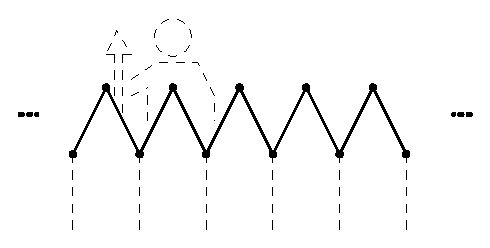
\includegraphics[width=100mm]{img/palisada.eps}
\[\xymatrix@R=7pt@C=14pt{& &-3\ \ar@{-}[ddl]\ar@{-}[ddr] & & -1\ \ar@{-}[ddl]\ar@{-}[ddr] & & \ 1\ \ar@{-}[ddl]\ar@{-}[ddr] & & \ 3\ \ar@{-}[ddl]\ar@{-}[ddr] \\ \cdots & & & & & & & & & & \cdots\\
& -4\  & & -2\  & & \ 0\  & & \ 2\ & & \ 4\ }\]
\caption{Obustronnie nieskończona palisada, czyli $\mathcal{C}$-korozbieralny $\mathcal{C}$-rdzeń z~przykładu \ref{buildable_not_dismantlable}.}\label{fig-palisada}
\end{figure}


\begin{problem}\label{prob1}
Czy $\mathcal{R}$-rozbieralność $X$~do~$A$, gdzie $\mathcal{R}\in\{\mathcal{I},\mathcal{C}\}$, implikuje \mbox{$\mathcal{R}$-korozbieralność} $X$~z~$A$~dla dowolnej pary przestrzeni Aleksandrowa $(X,A)$?
\end{problem}

Interesującą klasą częściowych porządków, zawierającą klasę porządków bez promieni, są rozważane na przykład przez Farleya \cite{Farley97} porządki bez nieskończonych łańcuchów i~\textit{jednostronnie nieskończonych palisad} (tj.~podzbiorów izomorficznych ze zbiorem $\mN$~z porządkiem zadanym jak w~przykładzie \ref{buildable_not_dismantlable} bądź z~porządkiem do niego dualnym). Naturalne wydaje się pytanie o~odpowiednik twierdzenia \ref{build_if_dism} dla tej klasy.

\begin{problem}\label{prob2}
Niech $X$~będzie przestrzenią Aleksandrowa nie zawierającą nieskończonych łańcuchów i~nieskończonych palisad, zaś $A$~jej podzbiorem. Czy $X\dism A$ wtedy i~tylko wtedy, gdy $A\codism X$?
\end{problem}

Niech $\left(s_{\phi+1,\phi}\colon A_{\phi+1}\to A_{\phi}\right)_{\phi<\beta}$ będzie ciągiem $\mathcal{R}$-korozbierającym przestrzeń $X$~z~$A$. Dla każdej liczby porządkowej $\psi\leq \beta$ określimy retrakcję $\revcomp\left(s_{\phi}\right)_{\psi\leq \phi<\beta}\colon X\to A_\psi$ zwaną \textit{nieskończonym złożeniem wstecz}\index{nieskonzzzczone zlzzzozzzzenie@nieskończone złożenie!wstecz}\nomenclature[7r]{$\revcomp\left(s_{\phi}\right)_{\psi\leq\phi<\beta}$}{nieskończone złożenie wstecz ciągu retrakcji $\left(s_{\phi}\colon X_{\phi+1}\to X_\phi\right)_{\psi\leq\phi<\beta}$} elementów ciągu $\left(s_{\phi+1,\phi}\right)_{\psi\leq \phi<\beta}$. W~tym celu zdefiniujemy najpierw pomocniczą \textit{funkcję skoku}\index{odwzorowanie!skoku}\index{funkcja!skoku}\label{def-nieskonczone_zlozenie_korozbierajacego_ciagu}
 $\s\left(s_{\phi+1,\phi}\right)_{\phi<\beta}\colon X\to X$\nomenclature[7ra]{$\s\left(s_{\phi}\right)_{\phi<\beta}$}{funkcja skoku związana z~ciągiem retrakcji $\left(s_{\phi}\colon X_{\phi+1}\to X_\phi\right)_{\phi<\beta}$}. Dla $x\in A$ niech $\s\left(s_{\phi+1,\phi}\right)_{\phi<\beta}(x)=x$. Natomiast dla $x\not\in A$ istnieje największa liczba porządkowa $0\leq \phi_x<\beta$ taka, że $x\not\in A_{\phi_x}$; przyjmujemy $\s\left(s_{\phi+1,\phi}\right)_{\phi<\beta}(x)=s_{\phi_{x}+1,\phi_{x}}(x)$. 

Dla $\psi\leq\beta$ oraz $x\in X$ niech \[\revcomp\left(s_{\phi+1,\phi}\right)_{\psi\leq \phi<\beta}(x)=\left(\s\left(s_{\phi+1,\phi}\right)_{\phi<\beta}(x)\right)^{n^x_\psi}(x),\] gdzie \[n_\psi^x=\min\left\{n\in\mN:\left(\s\left(s_{\phi+1,\phi}\right)_{\phi<\beta}(x)\right)^n(x)\in A_\psi\right\}.\]

\begin{lem}\label{lem-iteracje_s_na_x_tworza_skonczony_zbior}
Niech $(X,A)$~będzie parą przestrzeni Aleksandrowa, zaś $\left(s_{\phi+1,\phi}\colon A_{\phi+1}\to A_{\phi}\right)_{\phi<\beta}$ ciągiem $\mathcal{R}$-korozbierającym przestrzeń $X$~z~$A$. Wówczas dla każdego elementu $x\in X$ zbiór \[\left\{\left(\s\left(s_{\phi+1,\phi}\right)_{\phi<\beta}(x)\right)^n(x):n\in\mN\right\}=\left\{\revcomp\left(s_{\phi+1,\phi}\right)_{\psi\leq \phi<\beta}(x):\psi\leq\beta \right\}\] jest skończony.
\end{lem}
\begin{proof}
Dla elementu $x\in X$ niech \[\phi(x)=\min\left\{0\leq \phi<\beta:x\in A_{\phi}\right\}.\] 
Zauważmy, że dla każdego $x\in X\smallsetminus A$ zachodzi nierówność \[\phi\left(\s\left(s_{\phi+1,\phi}\right)_{\phi<\beta}(x)\right)< \phi(x).\] Zbiór \[\left\{\phi\left(\left(\s\left(s_{\phi+1,\phi}\right)_{\phi<\beta}\right)^n(x)\right):n\in\mN\right\}\] jest dobrze uporządkowany, więc nie zawiera nieskończonego łańcucha zstępującego; musi zatem być skończony. Ponadto $\s\left(s_{\phi+1,\phi}\right)_{\phi<\beta}\big|_A=\id_A$. Wobec tego skończony jest również zbiór \[\left\{\left(\s\left(s_{\phi+1,\phi}\right)_{\phi<\beta}(x)\right)^n(x):n\in\mN\right\}.\qedhere\]
\end{proof}

Następujący wynik jest dotyczącym korozbieralności odpowiednikiem lematu \ref{lem-Irozbieralny-wtw-Crozbieralny}.
\begin{lem}\label{lem-Ckorozb_wtw_Ikorozb}
Niech $(X,A)$~będzie parą przestrzeni Aleksandrowa bez nieskończonych łańcuchów. Następujące warunki są równoważne:
\begin{compactitem}
\item[1)] $A\codism X$;
\item[2)] przestrzeń $X$~jest $(\mathcal{U}\cup\mathcal{D})$-korozbieralna z~$A$;
\item[3)] przestrzeń $X$~jest $\mathcal{I}$-korozbieralna z~$A$;
\end{compactitem}
\end{lem}
\begin{proof}
1)$\implies$2)\,: Jak w~dowodzie lematu \ref{lem-Irozbieralny-wtw-Crozbieralny} każdą $\mathcal{C}$-retrakcję z~ciągu \mbox{$\mathcal{C}$-korozbierającego} $X$~z~$A$~możemy przedstawić jako złożenie dwóch \mbox{$(\mathcal{U}\cup\mathcal{D})$-retrakcji}.

2)$\implies$3)\,: Rozważmy $\mathcal{D}$-retrakcję $r\colon Y\to r(Y)$ określoną na przestrzeni Aleksandrowa bez nieskończonych łańcuchów $Y$ i~różną od $\id_{Y}$. Zbiór \[B=\{y\in Y:r(y)\not=y\}\] jest niepusty, zatem $\min(B)\not=\emptyset$, gdyż porządek $Y$~jest dobrze ufundowany. Jeżeli $y_0\in\min(B)$, to ponieważ $r(y_0)<y_0$ oraz $r(y)=y$ dla wszystkich $y<y_0$, punkt $y_0$~jest nieredukowalny nad punktem $r(y_0)$. Istnieje więc \mbox{$\mathcal{I}$-retrakcja} $r_0\colon r(Y)\cup\{y_0\}\to r(Y)$~przeprowadzająca punkt $y_0$ na $r(y_0)$. Ponadto funkcja $r'\colon Y\to r(Y)\cup\{y_0\}$ zadana dla $y\in Y$ wzorem \[r'(y)=\begin{cases}r(y) & \text{dla } y\not=y_0,\\y_0 & \text{dla } y=y_0\end{cases}\] jest $\mathcal{D}$-retrakcją. Korzystając z~tej obserwacji nietrudno udowodnić za pomocą indukcji pozaskończonej, że przestrzeń $Y$~jest \mbox{$\mathcal{I}$-korozbieralna} z~$r(Y)$. Stosując to rozumowanie (oraz rozumowanie dualne) do retrakcji z~ciągu \mbox{$(\mathcal{U}\cup\mathcal{D})$-korozbierającego} $X$~z~$A$~wykazuje się \mbox{$\mathcal{I}$-korozbieralność} $X$~z~$A$.

3)$\implies$1)\,: Oczywiste, gdyż $\mathcal{I}\subseteq \mathcal{C}$.
\end{proof}

Podobnie jak w~przypadku lematu \ref{lem-Irozbieralny-wtw-Crozbieralny}, dowód równoważności warunków 1)~i~2)~lematu \ref{lem-Ckorozb_wtw_Ikorozb} oraz wynikania warunku 1)~z~warunku 3)~nie wymaga założenia o~braku nieskończonych łańcuchów w~$X$.

%---------------------------------------------------------------
%---------------------------------------------------------------
%---------------------------------------------------------------



\subsection{Klasyfikacja typów homotopijnych przestrzeni Aleksandrowa bez promieni}
W~niniejszej sekcji udowodnimy twierdzenie rozszerzające podaną przez Stonga ,,klasyfikację'' typów homotopijnych skończonych przestrzeni topologicznych (twierdzenie \ref{tw-stonga}) na przestrzenie Aleksandrowa bez promieni.

Użyteczne okaże się przy tym pojęcie rzędu grafu prostego bez promieni, zdefiniowane przez Schmidta \cite{Schmidt83}. Przypomnimy je oraz niektóre jego własności w~oparciu o~popularyzujące to pojęcie opracowanie autorstwa Halina \cite{Halin98}.

Dla każdej liczby porządkowej $\phi$~definiujemy indukcyjnie pewną klasę grafów prostych $\mathcal{RL}(\phi)$ \cite[Definition 3.1]{Halin98} w~następujący sposób:
\begin{compactitem}
\item[---] $\mathcal{RL}(0)$ jest klasą grafów skończonych,
\item[---] jeżeli $\phi>0$, to graf $H$~należy do $\mathcal{RL}(\phi)$, jeśli istnieje skończony zbiór wierzchołków $F\subseteq H$ taki, że każda spójna składowa grafu $H-F$ należy do $\mathcal{RL}(\psi)$ dla pewnego $\psi<\phi$.
\end{compactitem}
Przez $\mathcal{RL}$~oznaczmy sumę wszystkich klas $\mathcal{RL}(\phi)$. Okazuje się, że graf $H$~należy do $\mathcal{RL}$~dokładnie wtedy, gdy jest grafem bez promieni \cite[Proposition 3.2]{Halin98}. Dla $H\in \mathcal{RL}$ \textit{rzędem}\index{rzazzzd grafu bez promieni@rząd grafu bez promieni} grafu $H$, oznaczanym symbolem $\ord(H)$\nomenclature[2k]{$\ord(G)$}{rząd grafu prostego bez promieni $G$}, nazywamy najmniejszą liczbę porządkową $\phi$~taką, że $H\in \mathcal{RL}(\phi)$. 

Dla nieskończonego grafu bez promieni $H$~istnieje najmniejszy (w~sensie inkluzji) skończony podzbiór $F$~zbioru wierzchołków tego grafu taki, że dla każdej spójnej składowej $D$~grafu $H-F$ zachodzi nierówność $\ord(D)<\ord(H)$ \cite[Lemma 3.11]{Halin98}. Zbiór $F$~o~powyższej własności nazywamy \textit{jądrem}\index{jazzzdro@jądro!grafu bez promieni} grafu $H$ \cite[Definition 3.12]{Halin98}~i~piszemy $\ker(H)=F$.\nomenclature[2j]{$\ker(G)$}{jądro grafu prostego bez promieni $G$} 

Dla częściowego porządku $P$~przyjmujemy oznaczenia $\ord(P)=\ord(\Comp(P))$ oraz $\ker(P)=\ker(\Comp(P))$.

Poniższe twierdzenie stanowi kluczową innowację bieżącego rozdziału w~stosunku do prac autora \cite{Kukiela10a,Kukiela10} i~pozwala na uogólnienie ich głównych wyników na wszystkie przestrzenie Aleksandrowa bez promieni. W~cytowanych pracach podobne twierdzenie \cite[wniosek III.2.2]{Kukiela10a}, \cite[Proposition 4.4]{Kukiela10} udowodnione zostało innymi metodami, ale jedynie dla przeliczalnych przestrzeni Aleksandrowa bez promieni oraz dla przestrzeni Aleksandrowa (dowolnej mocy), w~których wszystkie ścieżki proste są ograniczonej długości.

\begin{tw}\label{mocny_retrakt}
Jeśli $(X,A)$ jest $\Gamma$-parą przestrzeni Aleksandrowa bez promieni, to istnieje $\mathcal{C}$-rdzeń $(X^C,A)\subseteq (X,A)$, będący ekwiwariantnym mocnym retraktem deformacyjnym pary $(X,A)$ i~taki, że $X\dism^\Gamma X^C$.
\end{tw}
\begin{proof}
Przeprowadzimy indukcję ze względu na $\ord(X)$. %~oraz $\moc{\ker(X)}$. 

Załóżmy najpierw, że $\ord(X)=0$, co oznacza, że przestrzeń $X$~jest skończona. Jeśli $X=A$, nie mamy czego dowodzić. Załóżmy, że twierdzenie jest prawdziwe dla wszystkich par $(Y,A)$ takich, że $A\subseteq Y\subsetneq X$. Jeżeli $U_{(X,A)}=D_{(X,A)}=\id_X$, to wobec~lematu \ref{ciag_standardowy_staly_to_mamy_rdzen} para $(X,A)$ jest $\mathcal{C}$-rdzeniem. Jeśli jedna z~retrakcji $D_{(X,A)}$, $U_{(X,A)}$ nie jest tożsamościowa, oznaczmy ją przez $r\colon X\to r(X)$. Funkcja $r$~jest ekwiwariantną $\mathcal{C}$-retrakcją (lemat \ref{standardowy_jest_g}), więc \mbox{$X\dism^\Gamma r(X)$}. Na podstawie stwierdzenia \ref{stw-porownywalne_sa_homotopijne} istnieje homotopia $i\circ r\simeq \id_X\ \operatorname{rel} A$, gdzie $i\colon r(X)\hookrightarrow X$ jest włożeniem; nietrudno spostrzec, że jest ona ekwiwariantna. Ponieważ $r(X)\subsetneq X$, teza wynika z~założenia indukcyjnego.

Załóżmy, że $\ord(X)>0$ oraz twierdzenie jest prawdziwe dla każdej \mbox{$\Gamma$-pary} $(Y,B)$ przestrzeni Aleksandrowa bez promieni takiej, że $\ord(Y)<\ord(X)$. 

Przez $\left\{\hat{X}_i\right\}_{i\in I}$ oznaczmy indeksowaną rodzinę wszystkich składowych spójności przestrzeni $X\smallsetminus \ker(X)$. Zauważmy, że $\ord\left(\hat{X}_i\right)<\ord(X)$ dla każdego indeksu $i\in I$. Niech $A'=A\cup \ker(X)$; dla każdego indeksu $i\in I$ przyjmijmy oznaczenia $X_i=\hat{X}_i\cup \ker(X)$ oraz $A_i=X_i\cap A'$. Z~założenia indukcyjnego dla każdej z~przestrzeni $(X_i,A_i)$ istnieją zawarty w~niej $\mathcal{C}$-rdzeń $\left(X_i^C,A_i\right)$, liczba porządkowa $\alpha_i$, ciąg \[\left(r_i^{\phi,\phi+1}\colon X_i^{\phi}\to X_i^{\phi+1}\right)_{\phi<\alpha_i}\] retrakcji $\mcC$-rozbierający $X_i$~do~$X_i^C$ oraz mocna retrakcja deformacyjna $R_i\colon (X_i,A_i)\to \left(X_i^C,A_i\right)$.

Przyjmijmy oznaczenie $X^*=\bigcup_{i\in I}X_i^C$. Ponieważ $X_i\cap X_j=\ker(X)$ dla $i\not= j$ oraz $\bigcup_{i\in I}X_i=X$, funkcja $R=\bigcup_{i\in I} R_i\colon \left(X,A'\right)\to \left(X^*,A'\right)$ jest mocną retrakcją deformacyjną, a~ponadto para $(X^*,A')$ jest $\mathcal{C}$-rdzeniem. Niech \mbox{$\alpha=\max\{\alpha_i:i\in I\}$}. Dla $\alpha_i \leq \phi<\alpha$ przyjmijmy $r_i^{\phi,\phi+1}=\id_{X_i^{\alpha_i}}$. Wówczas \[\left(\bigcup_{i\in I}r_i^{\phi,\phi+1}\colon \bigcup_{i\in I}X_i^{\phi}\to \bigcup_{i\in I}X_i^{\phi+1}\right)_{\phi<\alpha}\] jest ciągiem $\mathcal{C}$-rozbierającym $X$~do zbioru $X^*$.

Co więcej, możemy retrakcje $R_i$~oraz $r_i^{\phi,\phi+1}$ dla $i\in I$, $\phi<\alpha_i$, dobrać tak, aby retrakcja deformacyjna $R$~oraz retrakcje~$\bigcup_{i\in I}r_i^{\phi,\phi+1}$ były zgodne z~działaniem grupy~$\Gamma$.

Przeprowadzimy indukcję ze względu na liczbę elementów zbioru $\ker(X)$. Jeśli $\moc{\ker(X)}=0$, to $A=A'$, a~zatem para $(X^*,A')=(X^*,A)$ jest $\mathcal{C}$-rdzeniem będącym mocnym retraktem deformacyjnym pary $(X,A)$, czyli teza twierdzenia zachodzi. 

Załóżmy, że twierdzenie jest prawdziwe dla wszystkich par $(Y,B)$ przestrzeni Aleksandrowa bez promieni o~tej własności, że $\ord(Y)=\ord(X)$ oraz $\moc{\ker(Y)}<\moc{\ker(X)}$. Rozważmy $\Gamma$-retrakcje $U_{(X^*,A)}$, $D_{(X^*,A)}$. Jeśli są one odwzorowaniami identycznościowymi, to $(X^*,A)$ jest $\mathcal{C}$-rdzeniem (lemat \ref{ciag_standardowy_staly_to_mamy_rdzen}), zaś $R$~szukaną retrakcją deformacyjną. Jeżeli natomiast jedno z~tych odwzorowań, oznaczmy je przez $\rho$, nie jest tożsamościowe, to istnieje punkt \mbox{$x\in X^*\smallsetminus A$} nieredukowalny w~$X^*$~i~taki, że $\rho(x)\not=x$. Ponieważ para $\left(X^*,A'\right)$ jest \mbox{$\mathcal{C}$-rdzeniem}, punkt \mbox{$x\not\in X^*\smallsetminus A'$}, a~zatem $x\in A'\smallsetminus A\subseteq \ker(X)$. Wobec tego $\moc{\ker\left(\rho\left(X^*\right)\right)}<\moc{\ker(X)}$. Z~założenia indukcyjnego istnieją $\mathcal{C}$-rdzeń $\left(X^C,A\right)$~oraz ekwiwariantna mocna retrakcja deformacyjna $S\colon \left(\rho\left(X^*\right),A\right)\to \left(X^C,A\right)$. Odwzorowanie \mbox{$(s\circ \rho\circ R)\colon (X,A)\to \left(X^C,A\right)$} jest ekwiwariantną mocną retrakcją deformacyjną. W~podobny sposób znajdujemy ciąg $\Gamma$-retrakcji $\mathcal{C}$-rozbierający $X$~do~$X^C$.
\end{proof}

Sama $\mathcal{C}$-rozbieralność przestrzeni Aleksandrowa bez promieni do $\mathcal{C}$-rdzenia jednoznacznego z~dokładnością do izomorfizmu jest dobrze znanym faktem \cite[Corollary 3.15]{Schroder99}.  Ważne w~twierdzeniu \ref{mocny_retrakt} jest istnienie mocnej retrakcji deformacyjnej na rdzeń.

Mówimy, że para przestrzeni Aleksandrowa $(X,A)$ jest \textit{lokalnie rdzeniem}\index{czezzzszzzciowy porzazzzdek@częściowy porządek!lokalnie rdzenzzz@lokalnie rdzeń}\index{rdzenzzz@rdzeń!(czezzzszzzciowy porzazzzdek)@(częściowy porządek)!lokalnie rdzenzzz@lokalnie rdzeń}, o~ile dla każdego $x\in X$ istnieje skończony zbiór $\lc_X(x)\subseteq X$\nomenclature[7o]{$\lc_X(x)$}{struktura lokalnego rdzenia wokół elementu $x$~zbioru częściowo uporządkowanego $X$} taki, że $x\in\lc_X(x)$ oraz spełnione są następujące warunki:
\begin{compactitem}
\item[---] jeśli $y\in\lc_X(x)\smallsetminus A$ oraz $y\not\in\min(X)$, to $\moc{\lc_X(x)\cap\max(y\mathord{\downarrow}_X\smallsetminus\{y\})}\geqslant 2$,
\item[---] jeśli $y\in\lc_X(x)\smallsetminus A$ oraz $y\not\in\max(X)$, to $\moc{\lc_X(x)\cap\min(y\mathord{\uparrow}_X\smallsetminus\{y\})}\geqslant 2$. 
\end{compactitem}

Dowody poniższych dwóch faktów przebiegają tak samo jak dowody cytowanych przy nich twierdzeń, dotyczących szczególnego przypadku, gdy zbiór $A$~jest pusty lub jednoelementowy.

\begin{tw}[{{\cite[twierdzenie III.2.3]{Kukiela10a}, \cite[Theorem 4.6]{Kukiela10}}}]\label{o_lokalnych_rdzeniach}Jeśli para przestrzeni Aleksandrowa $(X,A)$ jest lokalnie rdzeniem, to nie istnieje ciągłe odwzorowanie $f\colon (X,A)\to (X,A)$ takie, że $f\simeq \id_X \operatorname{rel} A$ oraz $f\not=\id_X$.
\end{tw}

\begin{stw}[{{\cite[twierdzenie III.2.5]{Kukiela10a}, \cite[Proposition 4.8]{Kukiela10}}}]\label{fp_rdzenie_sa_lokalne}
Jeśli para $(X,A)$ przestrzeni Aleksandrowa bez promieni jest $\mathcal{C}$-rdzeniem, to $(X,A)$ jest lokalnie rdzeniem.
\end{stw}

Z~twierdzenia \ref{o_lokalnych_rdzeniach} wynika, że jeśli para $(X,A)$ przestrzeni Aleksandrowa jest lokalnie rdzeniem, to jest $\mathcal{C}$-rdzeniem. Otrzymujemy z~niego natychmiast również  następujący wniosek.
\begin{wn}\label{lokalne_sa_dobre}
Jeśli pary przestrzeni Aleksandrowa $(X,A)$, $(Y,B)$ są lokalnie rdzeniami, zaś $f\colon (X,A)\to (Y,B)$, $g\colon (Y,B)\to (X,A)$ są ciągłymi odwzorwaniami takimi, że $g\circ f\simeq \id_X \operatorname{rel} A$ oraz $f\circ g\simeq \id_Y \operatorname{rel} B$, to $f,g$ są wzajemnie odwrotnymi homeomorfizmami.
\end{wn}

Poniższe twierdzenie, będące głównym wynikiem rozdziału, uogólnia na przestrzenie Aleksandrowa bez promieni podaną przez Stonga klasyfikację typów homotopijnych skończonych przestrzeni topologicznych (twierdzenie \ref{tw-stonga}) oraz wyniki uzyskane przez autora \cite{Kukiela10a,Kukiela10}.

\begin{tw}\label{wniosek_klasyfikacyjny}
Jeśli $X$, $Y$ są $\Gamma$-przestrzeniami Aleksandrowa bez promieni, to istnieją $\mathcal{C}$-rdzenie $X^C$, $Y^C$ będące ich ekwiwariantnymi mocnymi retraktami deformacyjnymi i~takie, że $X\dism^\Gamma X^C$ oraz $Y\dism^\Gamma Y^C$. Przestrzeń $X$~jest $\Gamma$-homotopijnie równoważna przestrzeni $Y$~wtedy i~tylko wtedy, gdy rdzenie $X^C$, $Y^C$ są $\Gamma$-homeomorficzne. 
\end{tw}
\begin{proof}
O~istnieniu $\mathcal{C}$-rdzeni $X^C$, $Y^C$~będących ekwiwariantnymi mocnymi retraktami deformacyjnymi $X$, $Y$~mówi twierdzenie \ref{mocny_retrakt}.

Ponieważ $X\simeq X^C$ oraz $Y\simeq Y^C$ w~sposób ekwiwariantny, z~istnienia \mbox{$\Gamma$-homeomorfizmu} $X^C\approx Y^C$ wynika $\Gamma$-homotopijna równoważność przestrzeni $X$, $Y$. 

Z~drugiej strony, istnienie $\Gamma$-homotopijnej równoważności przestrzeni $X$~oraz $Y$~implikuje istnienie $\Gamma$-homotopijnej równoważności pomiędzy $X^C$~a~$Y^C$. Wobec stwierdzenia \ref{fp_rdzenie_sa_lokalne} przestrzenie $X^C$, $Y^C$ są lokalnie rdzeniami. Zastosowanie wniosku \ref{lokalne_sa_dobre} kończy dowód.
\end{proof}

%---------------------------------------------------------------
%---------------------------------------------------------------
%---------------------------------------------------------------


\subsection{Wnioski z~twierdzenia klasyfikacyjnego}
Odnotujmy kilka wniosków z~rozważań poprzedniej sekcji. Rozpoczynamy od analogicznej jak w~przypadku skończonych przestrzeni topologicznych (por.~\cite[Corollary 4.9]{Barmak12}) charakteryzacji mocnych retraktów deformacyjnych przestrzeni Aleksandrowa bez promieni.

\begin{wn}\label{wn-charakteryzacja-mocnych-retraktow-deformacyjnych}
Niech $(X,A)$~będzie $\Gamma$-parą przestrzeni Aleksandrowa bez promieni. Następujące warunki są równoważne:
\begin{compactenum}
\item[1)] $A$~jest ekwiwariantnym mocnym retraktem deformacyjnym $X$;
\item[2)] $X\dism^{\Gamma} A$;
\item[3)] $A\codism^\Gamma X$.
\end{compactenum}
\end{wn}
\begin{proof}
Równoważność warunków 2) oraz 3) została wykazana w~twierdzeniu \ref{build_if_dism}. Wystarczy zatem udowodnić, że równoważne są warunki 1) i~2).

Zgodnie z~twierdzeniem \ref{mocny_retrakt} $X\dism^\Gamma X^C$ dla pewnej zawierającej zbiór $A$~podprzestrzeni $X^C\subseteq X$ takiej, że para $\left(X^C,A\right)$ jest $\mathcal{C}$-rdzeniem oraz istnieje ekwiwariantna mocna retrakcja deformacyjna $T\colon X\to X^C$.

Załóżmy, że $A$~jest ekwiwariantnym mocnym retraktem deformacyjnym $X$. Wówczas $(X^C,A)\simeq (A,A)$. Ponieważ pary $\left(X^C,A\right)$, $(A,A)$ są $\mathcal{C}$-rdzeniami, wobec stwierdzenia \ref{fp_rdzenie_sa_lokalne} oraz wniosku \ref{lokalne_sa_dobre} oznacza to, że $X^C=A$. Ale, jak zauważyliśmy, $X\dism^\Gamma X^C$.

Załóżmy, że $X\dism^\Gamma A$. Ustalmy liczbę porządkową $\alpha$~oraz \mbox{$\mathcal{C}$-rozbierający} $X$~do $A$~ciąg $\left(r_{\phi,\phi+1}\colon X_\phi\to X_{\phi+1}\right)_{\phi<\alpha}$ ekwiwariantnych retrakcji. Przyjmijmy oznaczenie $R=\infcomp\left(r_{\phi,\phi+1}\right)_{0\leq\phi<\alpha}\colon X\to A$. Wobec lematu \ref{lem-schroder_lemma} zachodzi równość $T\circ R\big|_{X^C}=\id_{X^C}$. Ale $R(X)=A$, zaś $T\big|_A=\id_A$, zatem $(T\circ R)\left(X^C\right)= A$. Stąd $X^C=A$.
\end{proof}
W~szczególności przestrzeń Aleksandrowa bez promieni jest ściągalna wtedy i~tylko wtedy, gdy pewien jej punkt jest jej mocnym retraktem deformacyjnym, co~jest z~kolei równoważne $\mathcal{C}$-rozbieralności do tego punktu. Częściowo odpowiada to na pytanie postawione przez autora \cite[Problem 5]{Kukiela10a}, \cite[Question 4]{Kukiela10}.
Nie jest jednak prawdą, że dowolny punkt ściągalnej przestrzeni Aleksandrowa bez promieni (a~nawet ściągalnej skończonej przestrzeni topologicznej) jest jej mocnym retraktem deformacyjnym. Kontrprzykład przedstawia rysunek \ref{fig-punkt_nie_bedacy_mocnym_retraktem_deformacyjnym}.

\begin{figure}[h]
\[
\xymatrix{\bullet\ar@{-}[d]\ar@{-}[drr] & \bullet\ar@{-}[dl]\ar@{-}[drr] & \bullet\ar@{-}[d]\ar@{-}[dr]\\
\!\!\!a\ \bullet\ar@{-}[drr] & & \bullet\ar@{-}[d]\ar@{-}[dr] & \bullet\ar@{-}[d]\ar@{-}[dl]\\
& & \bullet & \bullet}
\]
\caption{Diagram Hassego ściągalnej, skończonej przestrzeni topologicznej $X$~z~punktem wyróżnionym $a$~o~tej~własności, że $(X,\{a\})$ jest $\mcC$-rdzeniem, a~zatem przestrzeń $X$~nie jest $\mcC$-rozbieralna do $a$.}\label{fig-punkt_nie_bedacy_mocnym_retraktem_deformacyjnym}
\end{figure}

Wniosek \ref{wn-charakteryzacja-mocnych-retraktow-deformacyjnych} odpowiada również twierdząco na pytanie o~homotopijną równoważność przestrzeni Aleksandrowa bez promieni z~podzbiorem, do którego jest ona $\mcC$-rozbieralna~\cite[Problem 4]{Kukiela10a}, \cite[Question 3]{Kukiela10}.

Warto wspomnieć, że prawdziwe jest niniejsze stwierdzenie, będące uogólnieniem wyniku Stonga \cite{Stong84}. Jego dowód przebiega analogicznie jak dowód cytowanego przy nim słabszego odpowiednika z~pracy autora~\cite{Kukiela10}.
\begin{stw}[por.~{\cite[stwierdzenie III.3.4]{Kukiela10}}]
Załóżmy, że $X$, $Y$~są \mbox{$\Gamma$-przestrzeniami} Aleksandrowa bez promieni. Wówczas $\Gamma$-odwzorowanie $f:X\to Y$ jest $\Gamma$-homotopijną równoważnością wtedy i~tylko wtedy, gdy $f$~jest homotopijną równoważnością.
\end{stw}

Skupialiśmy się dotąd głównie na podobieństwach między skończonymi przestrzeniami topologicznymi a~przestrzeniami Aleksandrowa bez promieni. Pewną interesującą różnicę pomiędzy tymi klasami zauważyć można przyglądając się pojęciu homotopijnej dominacji. Przypomnijmy, że przestrzeń topologiczna $X$~\textit{homotopijnie dominuje}\index{homotopijna dominacja} nad przestrzenią topologiczną $Y$, co zapisujemy przez $X\geq_H Y$, o~ile istnieją ciągłe odwzorowania $f\colon X\to Y$, $g\colon Y\to X$ takie, że $f\circ g\simeq \id_Y$. Można udowodnić \cite[stwierdzenie III.3.1]{Kukiela10a}, że jeśli dla skończonych przestrzeni topologicznych $X$, $Y$~zachodzą homotopijne dominacje $X\geq_H Y$ oraz $Y\geq_H X$, to przestrzenie te są homotopijnie równoważne. Nie jest to prawdą dla dowolnych przestrzeni Aleksandrowa (patrz \cite[przykład III.3.2]{Kukiela10a}). Niżej wykazujemy, że fakt ten nie uogólnia się nawet na przestrzenie Aleksandrowa bez promieni. (Obserwacja ta wydaje się mieć bliski związek z~rozważaniami dotyczącymi tzw.~odwracalnych i~bijektywnie związanych częściowych porządków \cite{Kukiela09,Kukiela13a}.)

\begin{ex}
Dla $n\in\mN$ symbolem $A_n$~oznaczmy antyłańcuch o~$n$~elementach. Niech $K_{n,n}=A_n\oplus A_n$. Dla każdego $n\in\mN$ wybierzmy punkt wyróżniony $x_n\in \min(K_{n,n})$. Rozważmy przestrzenie ilorazowe \[X=\left(\coprod_{n\geq 1} K_{2n,2n}\right)\big/\{x_{2n}:n\in\mN\},\quad Y=\left(\coprod_{n\geq 1} K_{2n+1,2n+1}\right)\big/\{x_{2n+1}:n\in\mN\}.\] Łatwo zauważyć, że są one przestrzeniami Aleksandrowa bez promieni oraz \mbox{$\mathcal{C}$-rdzeniami}. Przestrzenie te nie są izomorficzne, a~zatem wobec twierdzenia \ref{wniosek_klasyfikacyjny} nie są homotopijnie równoważne. Widać jednak, że przestrzeń $X$~jest homeomorficzna pewnemu retraktowi przestrzeni $Y$, i~odwrotnie, $Y$~jest homeomorficzna retraktowi $X$. Zatem $X\geq_H Y$ oraz $Y\geq_H X$. 
\end{ex}


%---------------------------------------------------------------
%---------------------------------------------------------------
%---------------------------------------------------------------


\subsection{H-przestrzenie i~ko-H-przestrzenie Aleksandrowa bez promieni}
Przypomnijmy, że \textit{H-przestrzenią}\index{Hprzestrzenzzz@H-przestrzeń} nazywamy trójkę $(X,p,\mu)$ składającą się z~przestrzeni topologicznej $X$, jej wyróżnionego punktu $p\in X$ oraz ciągłego, zachowującego punkty wyróżnione odwzorowania $\mu:X\times X\to X$ o~tej własności, że diagram \[\xymatrix@C=60pt@R=40pt{X\ar[dr]_{\id_X}\ar[r]^{(p,\id_X)} & X\times X\ar[d]^{\mu} & X\ar[dl]^{\id_X}\ar[l]_{(\id_X,p)} \\ & X}\]
jest przemienny z~dokładnością do homotopii zachowującej punkty wyróżnione. Przez $p$~oznaczyliśmy w~powyższym diagramie odwzorowanie stałe.

Jeśli istnieje homotopijna równoważność $(X,p)\simeq (Y,q)$, to struktura \mbox{H-przestrzeni} na $X$ indukuje strukturę \mbox{H-przestrzeni} na $Y$ \cite[Theorem 1.5.4]{Spanier81}. Ponadto, jeśli przestrzeń $(X,p)$ jest ściągalna, to można na niej wprowadzić trywialne działanie $\mu:X\times X\to X$ takie, że $(X,p,\mu)$ jest H-przestrzenią: wystarczy przyjąć $\mu(x,y)=p$ dla wszystkich $x,y\in X$.

Stong~\cite{Stong66} udowodnił, że każda spójna, skończona H-przestrzeń jest ściągalna. Jego dowód przenosi się na przestrzenie Aleksandrowa bez promieni przy wykorzystaniu wyników niniejszej rozprawy prawie bez zmian. (W~dowodzie \cite[Proposition 13]{Stong66} należy jedynie zauważyć, że sumy zbiorów $D_r, D_r'$ zawierają nieskończone ścieżki proste.) Ponieważ jest on dość długi, nie przytaczamy go, poniższe twierdzenie pozostawiając bez dowodu.

\begin{stw}[por. {\cite[Section 5]{Stong66}}]\label{stw-stonga_o_h_przestrzeniach}
Niech $X$~będzie spójną przestrzenią Aleksandrowa bez promieni. Warunkiem koniecznym i~dostatecznym na to, by istniała struktura H-przestrzeni $(X,p,\mu)$ jest istnienie mocnej retrakcji deformacyjnej przestrzeni $X$~na przestrzeń jednoelementową $\{p\}$.
\end{stw}

Pojęciem dualnym do H-przestrzeni jest \textit{ko-H-przestrzeń}\index{ko-H-przestrzenzzz@ko-H-przestrzeń}, to jest trójka $(X,p,\eta)$ składająca się z~przestrzeni topologicznej $X$~z~punktem wyróżnionym $p\in X$ oraz ciągłego, zachowującego punkty wyróżnione odwzorowania $\eta\colon X\to X\vee X$ o~tej własności, 
że diagram
\[\xymatrix@C=60pt@R=40pt{X\ar@{<-}[dr]_{\id_X} & X\vee X\ar[l]_{\pi_1}\ar[r]^{\pi_2}\ar@{<-}[d]^{\eta} & X\ar@{<-}[dl]^{\id_X} \\ & X}\]
jest przemienny z~dokładnością do homotopii zachowującej punkty wyróżnione. W~powyższym diagramie $X\vee X=\{(x,y)\in X\times X: x=p \text{ lub } y=p\}$, zaś odwzorowania $\pi_1,\pi_2$ oznaczają rzuty odpowiednio na pierwszą i~drugą oś.

Podobnie jak ma to miejsce w~przypadku H-przestrzeni, jeżeli dana jest homotopijna równoważność $(X,p)\simeq (Y,q)$, to struktura ko-H-przestrzeni na $X$~wyznacza strukturę ko-H-przestrzeni na $Y$~\cite[Theorem 1.6.1]{Spanier81}. Jeśli przestrzeń $(X,p)$~jest ściągalna, to istnieje trywialne kodziałanie $\eta:X\to X\vee X$ (zadane dla wszystkich $x\in X$ wzorem $\eta(x)=(p, p)$) takie, że trójka $(X,p,\eta)$ jest \mbox{ko-H-przestrzenią}.

Helmstutler i~Vaughn \cite{Helmstutler10} wykazali, iż każda skończona ko-H-przestrzeń jest ściągalna. Podany przez nich prosty dowód zasadniczo różni się od dowodu wspomnianego wyżej wyniku Stonga, pomimo że same rezultaty wydają się dualne. Poniższe twierdzenie uogólnia twierdzenie Helmstutlera i~Vaughna na przestrzenie Aleksandrowa bez promieni.

\begin{stw}[por.~{\cite[Theorem 8]{Helmstutler10}}]\label{stw-helmsutlera-vaughna}
Niech $X$~będzie przestrzenią Aleksandrowa bez promieni. Warunkiem koniecznym i~dostatecznym na to, by istniała struktura ko-H-przestrzeni $(X,p,\eta)$ jest istnienie mocnej retrakcji deformacyjnej przestrzeni $X$~na przestrzeń jednoelementową $\{p\}$.
\end{stw}
\begin{proof}
Załóżmy, że istnieje struktura ko-H-przestrzeni $(X,p,\eta)$.
Wobec twierdzenia \ref{mocny_retrakt} istnieje $\mathcal{C}$-rdzeń $(X^C,p)$ będący mocnym retraktem deformacyjnym przestrzeni $(X,p)$. Na $X^C$ istnieje zatem struktura ko-H-przestrzeni $(X^C,p,\eta^C)$. Wykażemy, że $X^C=\{p\}$.

Ponieważ $\pi_1\circ \eta^C\simeq \id_{X^C}$ oraz $\pi_2\circ \eta^C \simeq \id_{X^C}$, z~twierdzeń \ref{o_lokalnych_rdzeniach}, \ref{fp_rdzenie_sa_lokalne} otrzymujemy $\pi_1\circ \eta^C=\id_{X^C}=\pi_2\circ \eta^C$.

Ustalmy $x\in X^C$. Wówczas $\eta^C(x)=(p,x')$ lub $\eta^C(x)=(x',p)$ dla pewnego elementu $x'\in X$. W~pierwszym przypadku mamy \[x=\id_{X^C}(x)=\left(\pi_1\circ\eta^C\right)(x)=p.\] Podobnie, w~drugim przypadku zachodzi równość $x=p$; stąd $X^C=\{p\}$.
\end{proof}

Powyższe twierdzenia oznaczają, że nie istnieje spójna, ale nieściągalna przestrzeń Aleksandrowa bez promieni $(X,p)$~taka, że dla każdej przestrzeni topologicznej z~punktem wyróżnionym $(Y,p)$ na  zbiorze klas homotopii $[(Y,q),(X,p)]$ lub na zbiorze $[(X,p),(Y,q)]$ istnieje naturalne działanie mające obustronny element neutralny \cite[Propositions 2.2.3, 2.2.9]{Arkowitz11}. W~szczególności na zbiorach tych nie istnieje naturalna struktura grupy.

Dodajmy, że Hardie, Vermeulen i~Witbooi \cite{Hardie02} rozpatrywali skończone przestrzenie topologiczne bedące ,,skończonymi modelami'' nietrywialnych \mbox{H-przestrzeni}, spełniające odpowiednio osłabione aksjomaty \mbox{H-przestrzeni}.

%---------------------------------------------------------------
%---------------------------------------------------------------
%---------------------------------------------------------------


\subsection{Słabsze formy rozbieralności przestrzeni Aleksandrowa}
Niech $\mathcal{R}$~będzie ustaloną klasą retrakcji w~kategorii przestrzeni Aleksandrowa. Przestrzeń Aleksandrowa nazywamy \textit{lokalnie $\mathcal{R}$-rozbieralną}\index{czezzzszzzciowy porzazzzdek@częściowy porządek!lokalnie rozbieralny}, jeżeli każdy jej skończony podzbiór zawiera się w~skończonym, $\mathcal{R}$-rozbieralnym podzbiorze tej przestrzeni. Podobną definicję w~przypadku grafów prostych podali np.~Hensel, Osajda i~Przytycki \cite{Hensel14}. Wyniki bieżącej sekcji zainspirowane są postawionym przez nich problemem \cite[Question 2.11]{Hensel14}, którego rozwiązanie (korzystające z~tych wyników) znajduje się w~rozdziale \ref{chap5}.

Wobec lematu \ref{lem-Irozbieralny-wtw-Crozbieralny} lokalna $\mathcal{I}$-rozbieralność jest równoważna lokalnej \mbox{$\mathcal{C}$-rozbieralności}. Ponieważ nie będziemy zajmować się lokalną \mbox{$\mathcal{R}$-rozbieralnością} dla $\mathcal{R}\not\in\{\mathcal{C},\mathcal{I}\}$, o~przestrzeni lokalnie \mbox{$\mathcal{C}$-rozbieralnej} mówimy krótko, że jest \textit{lokalnie rozbieralna}.

\begin{lem}\label{lem-rozb_to_slabo_rozb}
Niech $X$~będzie przestrzenią Aleksandrowa. Jeżeli $X\dism *$ lub $*\codism X$, to przestrzeń $X$~jest lokalnie rozbieralna.
\end{lem}
\begin{proof}
Ustalmy skończony podzbiór $D\subseteq X$.

Załóżmy, że $X\dism *$. Ustalmy liczbę porządkową $\alpha$ oraz $\mathcal{C}$-rozbierający $X$~do punktu ciąg $\left(r_{\phi,\phi+1}\right)_{\phi<\alpha}$. Zbiór \[\bigcup_{0\leq \psi<\alpha}\left(\infcomp\left(r_{\phi,\phi+1}\right)_{0\leq\phi<\psi}(D)\right)\] jest skończony (co wynika łatwo z~nieskończonej składalności ciągu \mbox{$\mathcal{C}$-rozbierającego}). Nietrudno spostrzec, że jest on \mbox{$\mathcal{C}$-rozbieralny}.

Podobnie, jeśli $*\codism X$ oraz $\left(s_{\phi+1,\phi}\right)_{\phi<\beta}$ jest, dla pewnej liczby porządkowej $\beta$, ciągiem $\mathcal{C}$-korozbierającym $X$~z~punktu, to~zbiór \[\bigcup_{0\leq \psi\leq \beta}\left(\revcomp\left(s_{\phi+1,\phi}\right)_{\psi\leq \phi<\beta}(D)\right)\] jest skończony (na podstawie lematu \ref{lem-iteracje_s_na_x_tworza_skonczony_zbior}) oraz $\mathcal{C}$-rozbieralny.
\end{proof}

\begin{figure}[h]
\[
\xymatrix@R=25pt@C=25pt{
&&		&		&		&		&		&		& 14\ar@{-}[d]\ar@{-}[dr]	& \widehat{14}\ar@{-}[d]\ar@{-}[dl]\\
&&		&		& 5\ar@{-}[d]\ar@{-}[dr]\ar@{-}[drr]	& \widehat{5}\ar@{-}[d]\ar@{-}[dl]\ar@{-}[drr]	&		&		& 13\ar@{-}[d]\ar@{-}[dr]\ar@{-}[dll]	& \widehat{13}\ar@{-}[d]\ar@{-}[dl]\ar@{-}[dll]\\
0\ar@{-}[drr] & \widehat{0}\ar@{-}[drr]	&	&		& 4\ar@{-}[d]\ar@{-}[dr]\ar@{-}[dll]\ar@{-}[drr]	& \widehat{4}\ar@{-}[d]\ar@{-}[dl]\ar@{-}[dll]\ar@{-}[drr]	& 6\ar@{-}[d]\ar@{-}[dr]	& \widehat{6}\ar@{-}[d]\ar@{-}[dl]	& 12\ar@{-}[d]\ar@{-}[dr]\ar@{-}[dll]	& \widehat{12}\ar@{-}[d]\ar@{-}[dl]\ar@{-}[dll] & \cdots\\
&&1\ar@{-}[d]\ar@{-}[dr]	& \widehat{1}\ar@{-}[d]\ar@{-}[dl]	& 3\ar@{-}[dll]\ar@{-}[drr]	& \widehat{3}\ar@{-}[dll]\ar@{-}[drr]	& 7\ar@{-}[d]\ar@{-}[dr]	& \widehat{7}\ar@{-}[d]\ar@{-}[dl]	& 11\ar@{-}[d]\ar@{-}[dr]\ar@{-}[dll]	& \widehat{11}\ar@{-}[d]\ar@{-}[dl]\ar@{-}[dll]\\
&&2		& \widehat{2}	& 		& 		& 8\ar@{-}[d]\ar@{-}[dr]	& \widehat{8}\ar@{-}[d]\ar@{-}[dl]	& 10\ar@{-}[dll]	& \widehat{10}\ar@{-}[dll]\\
&&		&		&		&		& 9	& \widehat{9}}
\]
\caption{Diagram Hassego lokalnie rozbieralnego częściowego porządku, który nie jest $\mathcal{C}$-rozbieralny ani $\mathcal{C}$-korozbieralny.}\label{slabo_rozb_ale_nie_rozb}
\end{figure}

\begin{ex}\label{ex-slabo_rozb_ale_nie_rozb}
Nie jest prawdą, że jeśli przestrzeń Aleksandrowa $X$~jest lokalnie rozbieralna, to $X\dism *$ lub $*\codism X$. Niech $X$~oznacza częściowy porządek, którego diagram Hassego przedstawiony jest na rysunku \ref{slabo_rozb_ale_nie_rozb}. Zauważmy, że jest on sumą wstępującego ciągu swoich skończonych, $\mathcal{I}$-rozbieralnych podzbiorów:
\[X=\bigcup_{n\in\mN} \left(\left\{m:0\leq m\leq a_n\right\}\cup \bigl\{\widehat{m}:0\leq m< a_n\bigr\}\right),\]
gdzie $a_0=0$ oraz $a_n=a_{n-1}+n+1$ dla $n\geq 1$. Przestrzeń $X$~jest zatem lokalnie rozbieralna. Nietrudno sprawdzić, że przestrzeń nie jest ona $\mathcal{C}$-rozbieralna ani $\mathcal{C}$-korozbieralna.
\end{ex}

\begin{comment}\begin{lem}\label{lem-retrakcje_zachowuja_slaba_rozbieralnosc}
Jeżeli przestrzeń Aleksandrowa~jest lokalnie rozbieralna, to każdy jej retrakt jest również lokalnie rozbieralny.
\end{lem}
\begin{proof}
Niech $X$~będzie lokalnie rozbieralną przestrzenią Aleksandrowa, zaś $r\colon X\to A$ zachowującą porządek retrakcją. Ustalmy skończony zbiór $D\subseteq A$. Ponieważ $A\subseteq X$, zbiór $D\subseteq X$. Istnieje zatem skończony, $\mathcal{I}$-rozbieralny zbiór $E\subseteq X$ zawierający $D$; niech $\left(r_i\colon E_i\to E_{i+1}\right)_{i=1}^{n}$ będzie, dla pewnej liczby $n\in\mN$, ciągiem $\mathcal{I}$-rozbierającym $E$~do punktu. Zbiór $r(E)$ jest skończony, zawiera $D$, a~$\bigl((r\circ r_i)\colon r(E_i)\to r(E_{i+1})\bigr)_{i=1}^{n}$ jest ciągiem $\mathcal{C}$-rozbierającym ten zbiór do punktu.
DOWÓD ZŁY. ALE Z INNYCH PRZYCZYN TAK CHYBA JEST - BO RETRAKT SKONCZONEGO ROZBIERALNEGO JEST ROZBIERALNY
\end{proof}
\end{comment}

Mówimy, że niepusta przestrzeń Aleksandrowa $X$~jest \mbox{\textit{s-ściągalna}}\index{sszzzciazzzgalnoszzzczzz@s-ściągalność}\index{czezzzszzzciowy porzazzzdek@częściowy porządek!sszzzciazzzgalny@s-ściągalny}, o~ile każde zachowujace porządek odwzorowanie skończonej przestrzeni topologicznej w~przestrzeń $X$~jest homotopijne z~odwzorowaniem stałym. 

\begin{lem}\label{lem-lok_rozb_to_s-sciagalna}
Jeżeli przestrzeń Aleksandrowa jest lokalnie rozbieralna, to jest \mbox{s-ściągalna}.
\end{lem}
\begin{proof}
Niech $X$~będzie lokalnie rozbieralną przestrzenią Aleksandrowa, $D$~skończoną przestrzenią topologiczną, zaś $f\colon D\to X$ zachowującym porządek odwzorowaniem. Zbiór $f(D)\subseteq X$ jest skończony, a~zatem istnieje skończony, \mbox{$\mathcal{C}$-rozbieralny} zbiór $A\subseteq X$ zawierający $f(D)$. Ponieważ przestrzeń $A$~jest ściągalna (patrz wniosek \ref{wn-charakteryzacja-mocnych-retraktow-deformacyjnych}) oraz $f(D)\subseteq A$, przekształcenie $f$~jest homotopijne z~funkcją stałą.
\end{proof}

Autor nie wie, czy istnieją s-ściągalne przestrzenie Aleksandrowa, które nie są lokalnie rozbieralne.

\begin{lem}\label{lem-retrakcje_zachowuja_s-sciagalnosc}
Jeżeli przestrzeń Aleksandrowa~jest s-ściągalna, to każdy jej retrakt również jest s-ściągalny.
\end{lem}
\begin{proof}
Niech $X$~będzie s-ściągalną przestrzenią Aleksandrowa, $r\colon X\to A$ zachowującą porządek retrakcją, zaś $i\colon A\hookrightarrow X$ włożeniem. Ustalmy skończoną przestrzeń topologiczną $D$ oraz zachowujące porządek odwzorowanie \mbox{$f\colon D\to A$}. Ponieważ przestrzeń $X$~jest s-ściągalna, istnieje homotopia \mbox{$h\colon X\times \I\to X$} między przekształceniem $(i\circ f)\colon D\to X$ a~pewną funkcją stałą $c\colon D\to X$. Odwzorowanie $\bigl(r\circ h \circ (i\times {\id_\I})\bigr)\colon A\times\I \to A$ jest homotopią między funkcją $(r\circ i\circ f)=f$ a~funkcją stałą $(r\circ c)\colon D\to A$.
\end{proof}

\begin{stw}\label{stw-rdzen_lokalny_s-sciagalny_to_punkt}
Jeżeli przestrzeń Aleksandrowa $X$~jest lokalnie rdzeniem, to jest s-ściągalna wtedy i~tylko wtedy, gdy jest jednoelementowa.
\end{stw}
\begin{proof}
Oczywiście przestrzeń jednoelementowa jest s-ściągalna, więc jedna z~implikacji jest trywialna.

Dla dowodu drugiej implikacji ustalmy przestrzeń Aleksandrowa $X$~będącą lokalnie rdzeniem, punkt $x\in X$ oraz zbiór $\lc_X(x)\subseteq X$. Niech $i\colon \lc_X(x)\hookrightarrow X$ będzie włożeniem. 

Wykażemy metodą indukcji, że jeśli $f\in \Cont(\lc_X(x),X)$ oraz $f\leq i$ w~porządku specjalizacji przestrzeni $\Cont(\lc_X(x),X)$ (tzn.~$f(y)\leq i(y)$ dla wszystkich $y\in \lc_X(x)$, patrz stwierdzenie \ref{stw-porzadek_na_cxy}), to $f=i$. Ustalmy w~tym celu zachowujące porządek odwzorowanie $f\colon \lc_X(x)\to X$ takie, że $f\leq i$. Jeśli $y\in \min(\lc_X(x))$, to z~własności zbioru $\lc_X(x)$ wynika, że $y\in \min(X)$, a~zatem $f(y)=y$. Niech $y\in \lc_X(x)\smallsetminus \min(\lc_X(x))$; załóżmy, że $f(z)=z$ dla wszystkich $z\in y\mathord{\downarrow}_{\lc_X(x)}$. Wobec własności zbioru $\lc_X(x)$ istnieją $z_1,z_2\in\lc_X(x)$, $z_1\not=z_2$, takie, że $z_1\prec y$ oraz $z_2\prec y$ w~porządku $X$. Ponieważ $z_1=f(z_1)\leq f(y)\leq y$, mamy $f(y)\in\{z_1,y\}$. Podobnie $f(y)\in\{z_2,y\}$; stąd $f(y)=y$. Wobec tego $f=i$. Analogicznie dowodzi się, że jeśli $f\in \Cont(\lc_X(x),X)$ oraz $f\geq i$, to $f=i$.

Na podstawie twierdzenia \ref{tw-kukiely-kiedy_cxy_aleksandrowa} przestrzeń $\Cont\left(\lc_X(x),X\right)$ jest Aleksandrowa. Wobec powyższych obserwacji oraz wniosku \ref{wn-stonga_o_skl_spojnosci} składowa łukowej spójności elementu $i\in \Cont(\lc_X(x),X)$ jest jednoelementowa. Zgodnie z~wnioskiem \ref{wn-homotopia_to_droga} oznacza to, że jeśli funkcja $f\colon \lc_X(x) \to X$ zachowuje porządek oraz $f\simeq i$, to $f=i$.

Załóżmy, że przestrzeń $X$~jest s-ściągalna. Jest ona zatem spójna (gdyż w~przeciwnym wypadku odwzorowanie dwuelementowej przestrzeni dyskretnej w~$X$~przeprowadzające elementy tej przestrzeni na punkty należące do dwóch rożnych składowych spójności $X$~nie byłoby homotopijne z~funkcją stałą). Włożenie $i\colon \lc_X(x)\hookrightarrow X$ jest homotopijne pewnej funkcji stałej $c\colon \lc_X(x)\to X$. Jak zauważyliśmy, oznacza to, iż $i=c$, a~zatem $\lc_X(x)$ jest zbiorem jednoelementowym, $\lc_X(x)=\{x\}$. Punkt $x$~jest wobec własności zbioru $\lc_X(x)$ jednocześnie maksymalny i~minimalny w~$X$. Ponieważ przestrzeń $X$~jest spójna, otrzymujemy $X=\{x\}$.
\end{proof}

\begin{comment}
\begin{lem}\label{lem-rdzen_lokalny_slabo_rozb_to_punkt}
Niech przestrzeń Aleksandrowa $X$~będzie $\mathcal{C}$-rdzeniem lokalnie. Przestrzeń $X$~jest lokalnie rozbieralna wtedy i~tylko wtedy, gdy jest jednoelementowa.
\end{lem}
\begin{proof}
Oczywiście każda przestrzeń jednoelementowa jest lokalnie rozbieralna, więc jedna z~implikacji lematu jest trywialna.

Dla dowodu drugiej implikacji ustalmy przestrzeń Aleksandrowa $X$~będącą rdzeniem lokalnie, punkt $x\in X$ oraz zbiór $\lc_X(x)$ o~własnościach jak w~definicji przestrzeni będącej rdzeniem lokalnie. Niech $D\subseteq X$ będzie skończonym zbiorem zawierającym~$\lc_X(x)$. Wobec własności zbioru $\lc_X(x)$ żaden element $y\in \lc_X(x)$ nie jest nieredukowalny w~$D$. Jeżeli więc $r\colon D\to r(D)$ jest $\mathcal{I}$-retrakcją, to $r\big|_{\lc_X(x)}=\id_{\lc_X(x)}$. Zatem $\lc_X(x)$ zawiera się w~każdym zbiorze, do którego zbiór $D$~jest $\mathcal{I}$-rozbieralny. 

Załóżmy, że przestrzeń $X$~jest lokalnie rozbieralna. Jest ona zatem spójna (gdyż w~przeciwnym wypadku jej podzbiór zawierający po jednym elemencie z~dwóch różnych składowych spójności nie zawierałby się w~żadnym $\mathcal{I}$-rozbieralnym podzbiorze $X$). Ponieważ przestrzeń $X$~jest lokalnie rozbieralna, istnieje skończony, $\mathcal{I}$-rozbieralny do punktu zbiór $D\subseteq X$ zawierający $\lc_X(x)$. Ale to oznacza, że $\lc_X(x)=\{x\}$~jest zbiorem jednoelementowym. Punkt $x$~jest wobec własności zbioru $\lc_X(x)$ jednocześnie maksymalny i~minimalny w~$X$. Ponieważ przestrzeń $X$~jest spójna, mamy $X=\{x\}$.
\end{proof}
\end{comment}

\begin{wn}\label{wn-rozbieralnosc_wtw_slaba_rozbieralnosc}
Niech $X$~będzie przestrzenią Aleksandrowa bez promieni. Następujące warunki są równoważne:
\begin{compactenum}
\item[1)] $X\dism *$;
\item[2)] przestrzeń $X$~jest lokalnie rozbieralna;
\item[3)] przestrzeń $X$~jest s-ściągalna.
\end{compactenum}
\end{wn}
\begin{proof}
Wynikanie warunku 2)~z~warunku 1)~oraz warunku 3)~z~warunku 2)~stanowi treść lematów \ref{lem-rozb_to_slabo_rozb} oraz \ref{lem-lok_rozb_to_s-sciagalna}.

Udowodnimy, że z~warunku 3)~wynika warunek 1). Załóżmy w~tym celu, że przestrzeń $X$~jest s-ściągalna. Wykażemy, iż $X\dism *$. Na podstawie stwierdzenia \ref{mocny_retrakt} istnieje $\mathcal{C}$-rdzeń $X^C\subseteq X$ taki, że $X\dism X^C$. Wobec stwierdzenia \ref{fp_rdzenie_sa_lokalne} jest on lokalnie rdzeniem. Z~lematu \ref{lem-retrakcje_zachowuja_s-sciagalnosc} wynika, że przestrzeń $X^C$~jest s-ściągalna, a~zatem $X^C$~jest, na podstawie stwierdzenia \ref{stw-rdzen_lokalny_s-sciagalny_to_punkt}, zbiorem jednoelementowym.
\end{proof}

\begin{comment}
\begin{stw}\label{tw-rozbieralnosc_wtw_slaba_rozbieralnosc}
Niech $X$~będzie przestrzenią Aleksandrowa bez promieni. Wówczas $X\dism *$ wtedy i~tylko wtedy, gdy przestrzeń $X$~jest lokalnie rozbieralna.
\end{stw}
\begin{proof}
Ze stwierdzenia \ref{stw-rozb_to_slabo_rozb} wiemy, że jeśli $X\dism *$, to przestrzeń $X$~jest lokalnie rozbieralna.

Załóżmy, że przestrzeń $X$~jest lokalnie rozbieralna. Udowodnimy, że $X\dism *$. Na podstawie stwierdzenia \ref{mocny_retrakt} istnieje $\mathcal{C}$-rdzeń $X^C\subseteq X$ taki, że $X\dism X^C$. Wobec stwierdzenia \ref{fp_rdzenie_sa_lokalne} jest on rdzeniem lokalnie. Z~lematu \ref{lem-retrakcje_zachowuja_slaba_rozbieralnosc} wynika, że przestrzeń $X^C$~jest lokalnie rozbieralna, a~zatem $X^C$~jest, na podstawie lematu \ref{lem-rdzen_lokalny_slabo_rozb_to_punkt}, zbiorem jednoelementowym.
\end{proof}
\end{comment}

%==============================================================
%==============================================================
%==============================================================

\section[Rozbieralność i~mocny typ homotopijny]{Rozbieralność i~mocny typ homotopijny kompleksów symplicjalnych}\label{sec-mocny_typ_homotopijny}%\sectionmark{Rozbieralność i~mocny typ homotopijny}

Celem niniejszego podrozdziału jest wprowadzenie pojęcia mocnego typu homotopijnego kompleksu symplicjalnego oraz podanie jego związków z~typem homotopijnym stowarzyszonej z~tym kompleksem przestrzeni Aleksandrowa. Wykorzystujemy przy tym przeniesione na kompleksy symplicjalne pojęcie rozbieralności. Rozważania te uogólniają niektóre wyniki pracy Barmaka i~Miniana~\cite{Barmak12}; zob.~też \cite{Fieux12}. Pojęcia mocnego typu homotopijnego i~rozbieralności skończonych kompleksów symplicjalnych rozpatrywane były przez kilku autorów pod inną nazwą i~w~innym kontekście \cite{Civan07,Matousek08}. Ponadto dla ogólniejszych obiektów określił je i~badał Matsushita~\cite{Matsushita14}.

\subsection{(Ko)rozbieralność kompleksów symplicjalnych}
Przypomnijmy (zob.~np.~\cite{Spanier81}), że odwzorowania symplicjalne $\varphi,\psi\colon K\to L$ nazywamy \textit{sąsiednimi}\index{sazzzsiedztwo@sąsiedztwo}\index{odwzorowanie!symplicjalne!sazzzsiednie@sąsiednie}\index{relacja!sazzzsiedztwa@sąsiedztwa}, jeżeli $\varphi(\sigma)\cup\psi(\sigma)$ jest sympleksem kompleksu $L$~dla każdego sympleksu $\sigma\in K$. Mówimy, że $\varphi,\psi$ leżą w~tej samej \textit{klasie sąsiedztwa}\index{klasa sazzzsiedztwa@klasa sąsiedztwa}, jeżeli istnieje skończony ciąg $\varphi=\varphi_0,\varphi_1,\ldots,\varphi_n=\psi$ odwzorowań symplicjalnych $K\to L$ taki, że $\varphi_i,\varphi_{i+1}$ są sąsiednie dla każdego $0\leq i<n$. Piszemy wówczas $\varphi\stackrel{\triangle}{\sim}\psi$.\nomenclature[7n]{$\varphi\stackrel{\triangle}{\sim}\psi$}{odwzorowania symplicjalne $\varphi,\psi$ leżą w~tej samej klasie sąsiedztwa} Nietrudno zauważyć, że jeśli $\varphi\stackrel{\triangle}{\sim}\psi$, to $|\varphi|\simeq |\psi|$. Odwrotna implikacja nie jest, oczywiście, prawdziwa. Przypomnijmy jednak \cite[Theorem 3.6.8]{Spanier81}, że jeśli $K,L$ są kompleksami symplicjalnymi oraz kompleks $K$~jest skończony, to można aproksymować klasy homotopii ciągłych odwzorowań $|K|\to |L|$ klasami sąsiedztwa odwzorowań symplicjalnych iterowanego podziału barycentrycznego kompleksu $K$~w~kompleks $L$.

Poniższe stwierdzenie, autorstwa Barmaka i~Miniana \cite{Barmak12}, podaje związek pomiędzy pojęciami sąsiedztwa odwzorowań symplicjalnych i~homotopii między ciągłymi przekształceniami skończonych przestrzeni topologicznych.

\begin{stw}[{\cite[Propositions 4.11, 4.12]{Barmak12}}]\label{porownywalny_to_sasiedni}
Niech $f,g\colon X\to Y$ będą ciągłymi odwzorowaniami skończonych przestrzeni topologicznych, zaś $\varphi, \psi\colon K\to L$ odwzorowaniami symplicjalnymi skończonych kompleksów symplicjalnych. Zachodzą następujące implikacje:
\begin{compactitem}
\item[---] jeżeli $\varphi\stackrel{\triangle}{\sim}\psi$, to $\mP(\varphi)\simeq \mP(\psi)$;
\item[---] jeżeli $f\simeq g$, to $\mK(f)\stackrel{\triangle}{\sim} \mK(g)$.
\end{compactitem}
\end{stw}

Stwierdzenie \ref{porownywalny_to_sasiedni} nie przenosi się bezpośrednio na przypadek nieskończonych kompleksów symplicjalnych i~przestrzeni Aleksandrowa: prawdziwa pozostaje jedynie pierwsza implikacja.

Zdefiniujemy pojęcia rdzenia oraz (ko)rozbieralności kompleksu symplicjalnego, wzorując się na ich odpowiednikach dla przestrzeni Aleksandrowa.

Niech $\mathcal{R}$~będzie pewną klasą retrakcji w~kategorii kompleksów i~odwzorowań symplicjalnych, $K$~niech będzie kompleksem symplicjalnym, zaś $L$~jego podkompleksem. Kompleks $K$~nazywamy \textit{$\mathcal{R}$-rdzeniem}\index{rdzenzzz@rdzeń!(kompleks symplicjalny)!r-rdzenzzz@$\mathcal{R}$-rdzeń}, jeśli nie istnieje różna od identyczności retrakcja $\rho\colon K\to \rho(K)$ należącą do $\mathcal{R}$.

Mówimy, że kompleks symplicjalny $K$~jest \textit{$\mathcal{R}$-rozbieralny do podkompleksu $L$}\index{rozbieralnoszzzczzz@rozbieralność!kompleksozzzw symplicjalnych@kompleksu symplicjalnego}\index{kompleks symplicjalny!rozbieralny}, jeżeli istnieją liczba porządkowa $\alpha$, ciąg pozaskończony $\left(K_\phi\right)_{\phi\leq\alpha}$ podkompleksów $K$~oraz nieskończenie składalny ciąg  pozaskończony należących do $\mathcal{R}$~retrakcji $\left(\rho_{\phi,\phi+1}\colon K_\phi \to K_{\phi+1}\right)_{\phi<\alpha}$, zwany \textit{ciągiem $\mathcal{R}$-rozbierającym $K$~do~$L$}\index{ciazzzg@ciąg!rrozbierajazzzcy@$\mathcal{R}$-rozbierający!kompleks symplicjalny do jego podkompleksu}, takie, że:\begin{compactitem}
\item[---] $K_0=K$;
%\item[---] $K_{\phi+1}=\rho_{\phi,\phi+1}(K_{\phi})$,
\item[---] $K_{\psi}=\bigcap_{\phi<\psi}K_{\phi}$ dla każdej granicznej liczby porządkowej $\psi\leq\alpha$;
\item[---] $K_\alpha=L$.
\end{compactitem}

Podobnie, mówimy że kompleks $K$~jest \textit{$\mathcal{R}$-korozbieralny z~$L$}\index{korozbieralnoszzzczzz@korozbieralność!kompleksu symplicjalnego}\index{kompleks symplicjalny!korozbieralny}, o~ile istnieją liczba porządkowa $\beta$, ciąg pozaskończony $\left(L_\phi\right)_{\phi\leq\beta}$ podkompleksów $K$~oraz ciąg pozaskończony, zwany \textit{ciągiem $\mathcal{R}$-korozbierającym $K$~z~$L$}\index{ciazzzg@ciąg!rkorozbierajazzzcy@$\mathcal{R}$-korozbierający!kompleks symplicjalny z~jego podkompleksu}, należących do $\mathcal{R}$~retrakcji $\left(\varsigma_{\phi+1,\phi}\colon L_{\phi+1} \to L_{\phi}\right)_{\phi<\beta}$ o~następujących własnościach:
\begin{compactitem}
\item[---] $L_0=L$;
\item[---] $L_{\psi}=\bigcup_{\phi<\psi}L_{\phi}$ dla każdej granicznej liczby porządkowej $\psi\leq\alpha$;
\item[---] $L_\beta=K$.
\end{compactitem}

Retrakcję $\rho\colon K\to \rho(K)$ taką, że jej złożenie $\iota\circ \rho\colon K\to K$ z~włożeniem \mbox{$\iota\colon \rho(K)\hookrightarrow K$} jest sąsiednie z~$\id_K$, nazywamy \textit{retrakcją sąsiednią}\index{retrakcja!sazzzsiednia@sąsiednia}. Klasę retrakcji sąsiednich oznaczmy przez $\mCtriang$\nomenclature[8b]{$\mCtriang$}{klasa retrakcji sąsiednich}; $\mCtriang$-rozbieralność $K$~do~$L$ oznaczamy symbolem $K\dism L$\nomenclature[7ga]{$K\dism L$}{kompleks symplicjalny $K$~jest $\mCtriang$-rozbieralny do podkompleksu $L$}, zaś $\mCtriang$-korozbieralnośc $K$~z~$L$ symbolem $L\codism K$\nomenclature[7ja]{$L\codism K$}{kompleks symplicjalny $K$~jest $\mCtriang$-korozbieralny z podkompleksu $L$}. Ponadto $\mCtriang$-rozbieralność $K$~do punktu oraz $\mCtriang$-korozbieralność $K$~z~punktu (nazywane również krótko $\mCtriang$-rozbieralnością oraz $\mCtriang$-korozbieralnością) oznaczamy odpowiednio symbolami $K\dism *$\nomenclature[7ia]{$K\dism *$}{kompleks symplicjalny $K$~jest $\mCtriang$-rozbieralny (do punktu)}, $*\codism K$\nomenclature[7la]{$*\codism K$}{kompleks symplicjalny $K$~jest $\mCtriang$-korozbieralny (z~punktu)}.

Mówimy, że wierzchołek $v\in K$ jest \textit{zdominowany}\index{wierzcholzzzek zdominowany@wierzchołek zdominowany} \cite{Barmak12} przez wierzchołek $v'\in K$, $v'\not=v$, jeżeli $\lk_K(v)$ jest stożkiem o~wierzchołku $v'$, tzn.~$\{v'\}\cup \sigma$ jest sympleksem w~$\lk_K(v)$ dla każdego sympleksu $\sigma\in \lk_K(v)$. Zdominowane wierzchołki są ,,symplicjalnym odpowiednikiem'' punktów nieredukowalnych.

Jeżeli $v\in K$ jest wierzchołkiem zdominowanym przez $v'\in K$, to retrakcję sąsiednią $\rho\colon K\to K-v$ zadaną dla wierzchołka $w\in K$~wzorem \[\rho(w)=\begin{cases}w & \text{dla } w\not=v,\\ v' & \text{dla } w=v\end{cases}\] nazywamy \textit{retrakcją usuwającą wierzchołek zdominowany}\index{retrakcja!usuwajazzzca@usuwająca!wierzcholzzzek zdominowany@wierzchołek zdominowany}. Klasę retrakcji usuwających wierzchołek zdominowany oznaczamy symbolem $\mItriang$.\nomenclature[8e]{$\mItriang$}{klasa retrakcji usuwających wierzchołek zdominowany}

Mówimy, że kompleks symplicjalny \textit{nie zawiera nieskończonego sympleksu}\index{kompleks symplicjalny!nie zawiera nieskonzzzczonego sympleksu@nie zawiera nieskończonego sympleksu}, jeśli nie istnieje nieskończony podzbiór $S$~zbioru wierzchołków kompleksu $K$~taki, że każdy skończony, niepusty podzbiór zbioru $S$~jest sympleksem $K$. Warunek ten jest równoważny temu, że każdy sympleks kompleksu $K$~zawarty jest w~maksymalnym sympleksie tego kompleksu. Zauważmy, że jeśli $v\in K$ jest wierzchołkiem kompleksu $K$~nie zawierającego nieskończonego sympleksu, to $v$~jest zdominowany przez $v'\in K$ wtedy i~tylko wtedy, gdy każdy maksymalny sympleks kompleksu $K$~zawierający $v$~zawiera również $v'$ (por.~\cite[Remark 2.2]{Barmak12}). 

\begin{comment}
\begin{lem}[por. {\cite[Propositions 2.7, 2.9]{Barmak12}}]\label{lem-Ctriang-rdzenie-charakteryzacja}
Załóżmy, że kompleks symplicjalny $K$~nie zawiera nieskończonego sympleksu. Następujące warunki są równoważne:
\begin{compactitem}
\item[1)] $K$~jest $\mCtriang$-rdzeniem;
\item[2)] nie istnieje zdominowany wierzchołek $v\in K$, tzn.~$K$~jest $\mItriang$-rdzeniem;
\item[3)] nie istnieje odwzorowanie symplicjalne $\phi\colon K\to K$ takie, że $\phi\stackrel{\triangle}{\sim}\id_K$ oraz $\phi\not=\id_K$.
\end{compactitem}
\end{lem}
\begin{proof}
1)$\implies$2)\,: Oczywiste, gdyż $\mItriang\subseteq \mCtriang$.

2)$\implies$3)\,: Załóżmy, że $K$~nie zawiera zdominowanego wierzchołka. Niech $\phi\colon K\to K$ będzie odwzorowaniem symplicjalnym sąsiednim $\id_K$. Ustalmy dowolny wierzchołek $v\in K$. Niech $\sigma$~będzie dowolnym maksymalnym sympleksem zawierającym $v$. Zbiór $\phi(\sigma)\cup\sigma$ jest sympleksem w~$K$. Wobec maksymalności $\sigma$~zachodzi równość $\sigma\cup\phi(\sigma)=\sigma$, stąd $\phi(v)\in \sigma$. Wierzchołek $\phi(v)$~należy wobec dowolności wyboru $\sigma$~do każdego maksymalnego sympleksu zawierającego $v$. Ponieważ $K$~nie zawiera zdominowanego wierzchołka, ma miejsce równość $v=\phi(v)$. Wobec dowolności wyboru wierzchołka $v$~otrzymujemy $\phi=\id_K$. Zatem jedynym odwzorowaniem należącym do klasy sąsiedztwa $\id_K$ jest $\id_K$.

3)$\implies$1)\,: Oczywiste.
\end{proof}
\end{comment}

\begin{lem}\label{lem-odwz_sasiednie_wierzcholek_zdominowany}
Niech $K$~będzie kompleksem symplicjalnym, zaś $\varphi\colon K\to K$ odwzorowaniem symplicjalnym. Jeśli $\varphi$~jest sąsiednie z~$\id_K$, to każdy wierzchołek $v\in K$ taki, że $\varphi(v)\not=v$, jest zdominowany przez wierzchołek $\varphi(v)$.
\end{lem}
\begin{proof}
Załóżmy, że $\varphi$~jest sąsiednie z~$\id_K$. Rozważmy wierzchołek $v\in K$ taki, że $\varphi(v)\not=v$. Niech $\sigma$~będzie sympleksem $\lk_K(v)$. Zbiór $\varphi(\sigma\cup\{v\})\cup(\sigma\cup\{v\})$ jest sympleksem w~$K$, a~zatem sympleksami w~$K$~są również jego podzbiory $\{v\}\cup \{\varphi(v)\}\cup\sigma$ oraz $\{\varphi(v)\}\cup\sigma$. Oznacza to, że $\{\varphi(v)\}\cup\sigma$ jest sympleksem $\lk_K(v)$. Wobec dowolności wyboru sympleksu $\sigma$~kompleks $\lk_K(v)$ jest stożkiem o~wierzchołku $\varphi(v)$. Wierzchołek $v$~jest zatem zdominowany przez $\varphi(v)$.
\end{proof}

\begin{lem}\label{lem-mCtriang-rozbieralnosc-wtw-mItriang-rozbieralnosc}
Niech $K$~będzie kompleksem symplicjalnym, zaś $L$~jego podkompleksem. Wówczas $K\dism L$ wtedy i~tylko wtedy, gdy kompleks $K$~jest $\mItriang$-rozbieralny do $L$.
\end{lem}
\begin{proof}
Ponieważ $\mItriang\subseteq \mCtriang$, to $\mItriang$-rozbieralność $K$~do $L$~implikuje, że $K\dism L$.

Dla dowodu przeciwnej implikacji rozważmy $\mCtriang$-retrakcję $\rho\colon K\to \rho(K)$. Ustawmy wierzchołki kompleksu $K$~nie należące do $\rho(K)$~w~ciąg pozaskończony $\left(v_\phi\right)_{\phi<\alpha}$. Dla $\phi\leq\alpha$ niech $K_\phi=K - \left\{v_\psi:\psi<\phi\right\}$.

Z~lematu \ref{lem-odwz_sasiednie_wierzcholek_zdominowany} wiemy, że wierzchołek $v_\phi\in K$ jest zdominowany przez $\rho(v_\phi)$. Ponieważ wierzchołki $v_\phi,\ \rho(v_\phi)\in K_{\phi}$, wierzchołek $v_\phi$~jest zdominowany przez $\rho(v_\phi)$~również w~kompleksie $K_\phi$. Istnieje zatem $\mItriang$-retrakcja $\rho_{\phi,\phi+1}\colon K_{\phi}\to K_{\phi+1}$ przeprowadzająca $v_\phi$ na $\rho(v_\phi)$.

Zauważmy, że nieskończone złożenie $\infcomp\left(\rho_{\phi,\phi+1}\right)_{0\leq\phi<\alpha}$ istnieje i~jest równe retrakcji $\rho$. Jeśli więc $K\dism L$, to każdą $\mCtriang$-retrakcję w~ciągu $\mCtriang$-rozbierającym $K$~do $L$~zastąpić można ciągiem pozaskończonym $\mItriang$-retrakcji, uzyskując w~ten sposób ciąg $\mItriang$-rozbierający $K$~do $L$.
\end{proof}

\begin{lem}[por. {\cite[Propositions 2.7, 2.9]{Barmak12}}]\label{lem-Ctriang-rdzenie-charakteryzacja}
Niech $K$~będzie kompleksem symplicjalnym. Następujące warunki są równoważne:
\begin{compactitem}
\item[1)] $K$~jest $\mCtriang$-rdzeniem;
\item[2)] nie istnieje zdominowany wierzchołek $v\in K$, tzn.~$K$~jest $\mItriang$-rdzeniem;
\item[3)] nie istnieje odwzorowanie symplicjalne $\varphi\colon K\to K$ takie, że $\varphi\stackrel{\triangle}{\sim}\id_K$ oraz $\varphi\not=\id_K$.
\end{compactitem}
\end{lem}
\begin{proof}
1)$\implies$2)\,: Oczywiste, gdyż $\mItriang\subseteq \mCtriang$.

2)$\implies$3)\,: Natychmiastowy wniosek z~lematu \ref{lem-odwz_sasiednie_wierzcholek_zdominowany}.

3)$\implies$1)\,: Oczywiste.
\end{proof} 

Rozbieralność przestrzeni Aleksandrowa jest blisko związana z~rozbieralnością kompleksów symplicjalnych.

\begin{lem}[por.~{\cite[Theorem 4.14]{Barmak12}}]\label{lem-rozbieralnosc_tu_i_tu}
Niech $K$~będzie kompleksem symplicjalnym, zaś $L\subseteq K$ jego podkompleksem. Jeżeli $K\dism L$, to $\mP(K)\dism \mP(L)$. % WTEDY I TYLKO WTEDY? SZTUCZKA SCHRODERA?

Niech $X$~będzie przestrzenią Aleksandrowa bez nieskończonych łańcuchów, zaś $A\subseteq X$ jej podprzestrzenią. Jeżeli $X\dism A$, to $\mK(X)\dism \mK(A)$.
\end{lem}
\begin{proof}
Niech $K_0$~będzie podkompleksem $K$, zaś $\rho\colon K\to K_0$ retrakcją sąsiednią. Rozważmy funkcję zachowującą porządek $r'_\rho\colon \mP(K)\to r_\rho'(\mP(K))$ zadaną dla $\sigma\in\mP(K)$ wzorem $r_\rho'(\sigma)=\sigma\cup \rho(\sigma)$. Oczywiście $r_\rho'(\sigma)\geq \sigma$ dla każdego elementu $\sigma\in\mP(K)$. Ponadto \begin{align*}r_\rho'\left(r_\rho'(\sigma)\right)&=\sigma\cup\rho(\sigma)\cup\rho(\sigma\cup \rho(\sigma))\\&=\sigma\cup\rho(\sigma)\cup\rho(\rho(\sigma))=\sigma\cup\rho(\sigma)\cup\rho(\sigma)=r_\rho'(\sigma).\end{align*} Odwzorowanie $r_\rho'$~jest zatem \mbox{$\mathcal{U}$-retrakcją}. Funkcja \[r_\rho''=\mP(\rho)\big|_{r_\rho'(\mP(K))}\colon r_\rho'(\mP(K))\to \mP(K_0)\] jest \mbox{$\mathcal{D}$-retrakcją} oraz $\mP(\rho)=r_\rho''\circ r_\rho'$. Jeśli zatem $\left(\rho_{\phi,\phi+1}\colon K_\phi\to K_{\phi+1}\right)_{\phi<\alpha}$ jest ciągiem \mbox{$\mathcal{C}$-rozbierającym} $K$~do~$L$, to ciąg $\left(\mP\left(\rho_{\phi,\phi+1}\right)\colon \mP\left(K_\phi\right)\to \mP\left(K_{\phi+1}\right)\right)_{\phi<\alpha}$ jest nieskończenie składalny, a~po zastąpieniu w~nim, dla każdej liczby porządkowej $\phi<\alpha$, retrakcji $\mP\!\left(\rho_{\phi,\phi+1}\right)$ parą retrakcji $r_{\rho_{\phi,\phi+1}}', r_{\rho_{\phi,\phi+1}}''$ otrzymujemy ciąg \mbox{$(\mathcal{U}\cup\mathcal{D})$-rozbierający} $\mP(K)$ do $\mP(L)$.

Z~drugiej strony zauważmy, że jeśli $r\colon X\to X\smallsetminus\{x\}$ jest retrakcją usuwającą punkt nieredukowalny $x$, to $r(x)\sim y$ dla każdego elementu $y\in x\mathord{\uparrow}\cup x\mathord{\downarrow}$. Wobec tego $x$~jest wierzchołkiem zdominowanym przez $r(x)$~w~$\mK(X)$. Odwzorowanie \[\mK(r)\colon \mK(X)\to \mK(X\smallsetminus\{x\})=\mK(X)-x\] jest więc $\mItriang$-retrakcją. Załóżmy, że $X\dism A$. Na podstawie lematu \ref{lem-Irozbieralny-wtw-Crozbieralny} istnieją liczba porządkowa $\alpha$~oraz pozaskończony ciąg $\left(r_{\phi,\phi+1}\colon X_\phi\to X_{\phi+1}\right)_{\phi<\alpha}$ retrakcji $\mathcal{I}$-rozbierający $X$~do~$A$. Wobec powyższych obserwacji $\left(\mK\left(r_{\phi,\phi+1}\right)\colon \mK\left(X_\phi\right)\to \mK\left(X_{\phi+1}\right)\right)_{\phi<\alpha}$ jest ciągiem $\mItriang$-rozbierającym kompleks $\mK(X)$ do $\mK(A)$.
\end{proof}

\begin{lem}\label{nsk_skladalnosc_w_kompl_bez_promieni}
Niech $K$~będzie kompleksem symplicjalnym bez promieni, $\alpha$~liczbą porządkową, zaś $\left(K_\phi\right)_{\phi\leq\alpha}$ zstępującym ciągiem podkompleksów $K$ o~tej własności, że $K_0=K$ oraz $K_{\psi}=\bigcap_{\phi<\psi}K_{\phi}$ dla każdej granicznej liczby porządkowej $\psi\leq\alpha$. Wówczas każdy pozaskończony ciąg $\mCtriang$-retrakcji $\left(\rho_{\phi,\phi+1}\colon K_\phi\to K_{\phi+1}\right)_{\phi<\alpha}$ jest nieskończenie składalny.
\end{lem}
\begin{proof}
Ustalmy liczbę porządkową $\alpha$~oraz ciąg $\mCtriang$-retrakcji $\left(\rho_{\phi,\phi+1}\colon K_\phi\to K_{\phi+1}\right)_{\phi<\alpha}$. Ciąg $\left(\mP\left(\rho_{\phi,\phi+1}\right)\colon \mP\left(K_\phi\right)\to \mP\left(K_{\phi+1}\right)\right)_{\phi<\alpha}$ wyznacza ciąg $(\mathcal{U}\cup\mathcal{D})$-retrakcji określony jak w~dowodzie lematu \ref{lem-rozbieralnosc_tu_i_tu}, który wobec lematu \ref{nsk_skladalnosc_w_prz_bez_promieni} jest nieskończenie składalny; nieskończenie składalny jest więc także ciąg $(\rho_{\phi,\phi+1})_{\phi<\alpha}$.
\end{proof}

\begin{comment}
Jako wniosek z~dowodu otrzymujemy następujący lemat.
\begin{lem}\label{lem-mctriang_rozbieralnosc_implikuje_mitriang_rozbieralnosc}
Dla kompleksu symplicjalnego $K$~bez nieskończonych sympleksów oraz jego podkompleksu $L$~jeżeli $K\dism L$, to $\mK(\mP(K))$~jest $\mItriang$-rozbieralny do $\mK(\mP(L))$.
\end{compactenum}
\end{lem}
\begin{proof}
Jeżeli $K\dism L$, to ze stwierdzenia \ref{stw-rozbieralnosc_tu_i_tu} zachodzi $\mP(K)\dism \mP(L)$. Ponieważ $K$~nie zawiera nieskończonego sympleksu, $\mP(K)$ nie zawiera nieskończonego łańcucha. Wobec lematu \ref{lem-Irozbieralny-wtw-Crozbieralny} przestrzeń $\mP(K)$~jest $\mathcal{I}$-rozbieralna do $\mP(L)$. Jak w~dowodzie stwierdzenia \ref{stw-rozbieralnosc_tu_i_tu} wykazujemy, że kompleks $\mK(\mP(K))$ jest $\mItriang$-rozbieralny do $\mK(\mP(L))$.
\end{proof}
\end{comment}

Związek pomiędzy $\mcC$-rdzeniami przestrzeni Aleksandrowa a~$\mCtriang$-rdzeniami kompleksów symplicjalnych opisuje następujący lemat.
\begin{lem}[por.~{\cite[Proposition 4.17]{Barmak12}}]\label{lem-strong_collapsible_to_strong_collapsible}
Niech $K$~będzie kompleksem symplicjalny. Jeżeli $\mP(K)$~jest $\mcC$-rdzeniem, to $K$~jest $\mCtriang$-rdzeniem.

Niech $X$~będzie przestrzenią Aleksandrowa. Jeżeli $X$~jest \mbox{$\mcC$-rdzeniem}, to $\mK(X)$~jest $\mCtriang$-rdzeniem. Jeśli $X$~nie zawiera nieskończonych łańcuchów oraz $\mK(X)$ jest \mbox{$\mCtriang$-rdzeniem}, to $X$~jest $\mcC$-rdzeniem.
\end{lem}
\begin{proof}
Z~lematu \ref{lem-rozbieralnosc_tu_i_tu} wynika natychmiast, że jeśli $\mP(K)$~jest $\mcC$-rdzeniem, to $K$~jest $\mCtriang$-rdzeniem, oraz że jeśli $X$~nie zawiera nieskończonych łańcuchów i~$\mK(X)$~jest $\mCtriang$-rdzeniem, to $X$~jest $\mcC$-rdzeniem.

Jeżeli $\mK(X)$~nie jest $\mCtriang$-rdzeniem, to wobec lematu \ref{lem-Ctriang-rdzenie-charakteryzacja} kompleks $\mK(X)$~zawiera wierzchołek $v$~zdominowany przez różny od niego wierzchołek $v'$. Oznacza to, że jeśli $\sigma$~jest sympleksem $\mK(X)$ (czyli skończonym, niepustym łańcuchem zawartym w~$X$) oraz $v\in\sigma$, to $\sigma\cup\left\{v'\right\}\in\mK(P)$. Wobec tego każdy element $x\in X$ porównywalny z~$v$~jest także porównywalny z~$v'$; w~szczególności $v\sim v'$. Dla ustalenia uwagi załóżmy, że $v< v'$. Odwzorowanie $r\colon X\to r(X)$ zadane dla $x\in X$ wzorem \[r(x)=\begin{cases}v', &\text{gdy } v\leq x\leq v',\\ x&\text{w przeciwnym wypadku}\end{cases}\] jest nietrywialną $\mathcal{U}$-retrakcją. Wobec tego $X$~nie jest $\mathcal{C}$-rdzeniem.
\end{proof}
Istnieją skończone kompleksy symplicjalne będące \mbox{$\mCtriang$-rdzeniami}, których uporządkowane zbiory ścian nie są \mbox{$\mcC$-rdzeniami} (np.~kompleks przedstawiony w~pracy Barmaka i~Miniana \cite[Example 2.13]{Barmak12}).



%------------------------------------------------------------------
%------------------------------------------------------------------
%------------------------------------------------------------------



\subsection{Mocny typ homotopijny kompleksów symplicjalnych}
Niech $K,L$~będą kompleksami symplicjalnymi. Mówimy, że $K,L$ mają ten sam \textit{mocny typ homotopijny}\index{typ homotopijny!mocny}, co oznaczamy przez $K\stronghe L$, gdy istnieją kompleksy symplicjalne $K=K_0,K_1,\ldots,K_n=L$ takie, że dla każdego $0\leq i<n$ ma miejsce jedna z~zależności: \[K_i\dism K_{i+1},\quad K_i\codism K_{i+1},\quad K_{i+1}\dism K_i,\quad K_{i+1}\codism K_i.\]

Powyższa definicja jest uogólnieniem (patrz wniosek \ref{wn-nasz_mocny_typ_homotopijny_uogolnia_Barmaka}) pojęcia mocnego typu homotopijnego skończonych kompleksów symplicjalnych, wprowadzonego przez Barmaka i~Miniana \cite[Definition 2.1]{Barmak12}. Autor nie jest przekonany, że jest to ,,właściwe'' uogólnienie. W~niniejszej sekcji staramy się uzasadnić przyjętą definicję w~przypadku kompleksów symplicjalnych bez promieni. 

\begin{stw}[por.~{\cite[Remark 2.3]{Barmak12}}]\label{stw-izomorficzne_sa_she}
Jeśli kompleksy symplicjalne $K_1, K_2$ są izomorficzne, to $K_1 \stronghe K_2$.
\end{stw}
\begin{proof}
Załóżmy, że kompleksy symplicjalne $K_1=(V_{K_1},S_{K_1}), K_2=(V_{K_2},S_{K_2})$ są izomorficzne. Istnieje kompleks symplicjalny $L=(V_L,S_L)$~izomorficzny z~tymi kompleksami oraz~rozłączny z~każdym z~nich. Niech $i\in\{1,2\}$. Ustalmy izomorfizm symplicjalny $\varphi_i\colon K_i\to L$. Rozważmy kompleks symplicjalny $L_i=(V_{L_i},S_{L_i})$~o~zbiorze wierzchołków $V_{L_i}=V_{K_i}\cup V_L$ i~zbiorze sympleksów \[S_{L_i}=\{\sigma\subseteq V_{L_i}:\text{istnieje sympleks } \tau\in S_{K_i} \text{ taki, że } \sigma\subseteq \tau\cup\varphi_i(\tau)\}.\]
Określmy odwzorowania symplicjalne $\rho_i\colon L_i\to K_i$ oraz $\rho_i'\colon L_i\to L$, dla $v\in V_{L_i}$ przyjmując:
\[\rho_i(v)=\begin{cases}v & \text{dla } v\in V_{K_i},\\\varphi^{-1}_i(v) & \text{dla } v\in V_{L},\end{cases} \quad\quad\quad \rho_i'(v)=\begin{cases}\varphi_i(v) & \text{dla } v\in V_{K_i},\\v & \text{dla } v\in V_{L}.\end{cases}\]
Nietrudno sprawdzić, że $\rho_i, \rho_i'\in \mCtriang$, a~zatem \[K_1\codism L_1\dism L\codism L_2\dism K_2.\qedhere\]
\end{proof}

\begin{stw}\label{stw-zgniatalny_jest_sciagalny}
Niech $K$~będzie kompleksem symplicjalnym, zaś $L\subseteq K$ jego podkompleksem takim, że $K\dism L$ lub $L\codism K$. Wówczas $|L|$~jest mocnym retraktem deformacyjnym $|K|$.
\end{stw}
\begin{proof}
Jeżeli $L\codism K$, to teza stwierdzenia wynika z~lematów \ref{lem-wlozenie_hom_rown_to_retrakcja_sdr}, \ref{lem-o_nieskonczonym_skladaniu_homotopijnych_rownowaznosci}, stwierdzenia \ref{stw-domkniety_podzbior_anr_jest_korozwloknieniem}, i~prostej obserwacji, że realizacja geometryczna retrakcji sąsiedniej jest mocną retrakcją deformacyjną .

Jeśli natomiast $K\dism L$, to istnieją liczba porządkowa $\alpha$~oraz nieskończenie składalny ciąg retrakcji $\left(\rho_{\phi,\phi+1}\colon K_\phi\to K_{\phi+1}\right)_{\phi<\alpha}$, który $\mCtriang$-rozbiera $K$~do~$L$. Ich realizacje geometryczne $\left|\rho_{\phi,\phi+1}\right|\colon \left|K_\phi\right|\to \left|K_{\phi+1}\right|$ są mocnymi retrakcjami deformacyjnymi. Dla każdej liczby porządkowej $\psi\leq \alpha$ niech \mbox{$R_\psi=\infcomp\left(\rho_{\phi,\phi+1}\right)_{0\leq \phi\leq \psi}\colon K\to K_\psi$}.  Wykażemy, że dla każdej liczby porządkowej $\psi\leq\alpha$ przekształcenie $\left|R_\psi\right|\colon |K|\to \left|K_\psi\right|$ jest mocną retrakcją deformacyjną.

Ustalmy w~tym celu $\psi\leq\alpha$. Jeżeli $\psi=0$, nie mamy czego dowodzić. Załóżmy, że $\left|R_\phi\right|$~jest mocną retrakcją deformacyjną dla każdej liczby porządkowej $\phi<\psi$. Jeśli $\psi$~jest następnikiem, $\psi=\phi+1$, to $\left|R_\psi\right|=\left|\rho_{\phi,\phi+1}\right|\circ \left|R_\phi\right|$ jest mocną retrakcją deformacyjną jako złożenie takich retrakcji. 

Załóżmy, że $\psi$~jest graniczną liczbą porządkową. Jako retrakcja $\left|R_\psi\right|$~indukuje epimorfizm grup homotopii. Wykażemy, że $\pi_k\left(\left|R_\psi\right|,x_0\right)$ jest monomorfizmem dla wszystkich $k\geq 0$ oraz $x_0\in |K|$. Ustalmy element $[p]\in \pi_k(|K|,x_0)$ reprezentowany przez ciągłe przekształcenie $p\colon \S^k\to |K|$. Jeżeli $\pi_k\left(\left|R_\psi\right|,x_0\right)([p])=0$, to istnieje homotopia $H\colon \S^k\times \I\to |K_{\psi}|$ między funkcją $\left|R_\psi\right|\circ p$ a~odwzorowaniem stałym równym $x_0$.
Zauważmy, że zbiór $p(\S^k)\subseteq |K|$ jest zwarty, a~zatem jest zawarty w~pewnym zwartym podkompleksie $D\subseteq K$ (patrz lemat \ref{lem-cw_zwarty_podzbior_w_skonczonym_podkompleksie}). Ponieważ ciąg $\mCtriang$-rozbierający $K$~do $L$~jest nieskończenie składalny, $R_\psi\big|_D=R_\beta\big|_D$ dla pewnej liczby porządkowej $\beta<\psi$, czyli $\left|R_\psi\right|\circ p=\left|R_\beta\right|\circ p$. Niech $i\circ \left|K_\psi\right|\hookrightarrow \left|K_\beta\right|$ oznacza włożenie. Złożenie $i\circ H$~jest homotopią między $\left|R_\beta\right|\circ p$ a~przekształceniem stałym, co oznacza, że $\pi_k\left(\left|R_\beta\right|,x_0\right)([p])=0$. Ponieważ $\pi_k\left(\left|R_\beta\right|,x_0\right)$ jest z~założenia indukcyjnego izomorfizmem, $[p]=0$~w~$\pi_k(|K|,x_0)$. Zatem $\pi_k\left(\left|R_\psi\right|,x_0\right)$ jest izomorfizmem. Korzystając z~twierdzenia Whiteheada \ref{tw-twierdzenie_whiteheada}, stwierdzenia \ref{stw-domkniety_podzbior_anr_jest_korozwloknieniem} oraz lematu \ref{lem-wlozenie_hom_rown_to_retrakcja_sdr} otrzymujemy tezę.
\end{proof}
\begin{wn}
Jeżeli $K\stronghe L$, to $|K|\simeq |L|$.
\end{wn}

\begin{uw}\label{uw-he_nie_implikuje_stronghe}
Nie jest prawdą, że jeśli $|K|\simeq |L|$, to istnieją takie triangulacje $K',L'$ wielościanów $|K|,|L|$, że $K'\stronghe L'$. Dowód tego faktu odkładamy do strony \pageref{dowod-uw-he_nie_implikuje_stronghe}.
\end{uw}

Niech $\varphi,\psi\colon K\to L$ będą odwzorowaniami symplicjalnymi. Mówimy, że odwzorowania $\varphi,\psi$ są \textit{$\infty$-sąsiednie}\index{sazzzsiedztwo@sąsiedztwo!0-sazzzsiedztwo@$\infty$-sąsiedztwo}\index{odwzorowanie!symplicjalne!0-sazzzsiednie@$\infty$-sąsiednie}\index{relacja!0-sazzzsiedztwa@$\infty$-sąsiedztwa}\index{0sazzzsiedztwo@$\infty$-sąsiedztwo}, jeśli istnieją liczba porządkowa $\alpha$~oraz ciąg pozaskończony odwzorowań symplicjalnych $\left(\varphi_\xi\colon K\to L\right)_{\xi\leq\alpha}$, zwany \textit{świadkiem \mbox{$\infty$-sąsiedztwa} $\varphi$~i~$\psi$}\index{szzzwiadek 0sazzzsiedztwa@świadek $\infty$-sąsiedztwa}, takie, że spełnione są następujące warunki:
\begin{compactitem}
\item[---] $\varphi_0=\varphi$;
\item[---] $\varphi_\alpha=\psi$;
\item[---] odwzorowania $\varphi_{\xi}$ oraz $\varphi_{\xi+1}$ są sąsiednie dla każdej liczby porządkowej $\xi<\alpha$;
\item[---] dla każdego wierzchołka $v\in K$ oraz każdej granicznej liczby porządkowej $\gamma\leq \alpha$ istnieje liczba porządkowa $\delta<\gamma$ o~tej własności, że $\varphi_{\xi}(v)=\varphi_{\gamma}(v)$ dla każdej liczby porządkowej $\delta\leq \xi\leq \gamma$.
\end{compactitem}
Niech $\stackrel{\infty}{\sim}$\nomenclature[7m]{$\varphi\stackrel{\infty}{\sim}\psi$}{odwzorowania symplicjalne $\varphi, \psi$ są równoważne w~sensie relacji równoważności generowanej przez relację $\infty$-sąsiedztwa} będzie najmniejszą relacją równoważności na zbiorze odwzorowań symplicjalnych $K\to L$ zawierającą wszystkie pary $(\varphi,\psi)$ odwzorowań $\infty$-sąsiednich. Oczywiście relacja $\stackrel{\infty}{\sim}$ zawiera relację $\stackrel{\triangle}{\sim}$. Ponadto, jeżeli kompleksy $K,L$ są skończone, to relacje te są identyczne. 

Następująca obserwacja jest natychmiastową konsekwencją powyższej definicji.
\begin{lem}\label{lem-stackrel_zgodny_ze_zlozeniami}
Jeżeli $\varphi_1,\varphi_2\colon K\to L$ oraz $\psi_1,\psi_2\colon L\to M$ są odwzorowaniami symplicjalnymi takimi, że $\varphi_1\stackrel{\infty}{\sim}\varphi_2$ oraz~$\psi_1\stackrel{\infty}{\sim}\psi_2$, to również $\psi_1\circ \varphi_1\stackrel{\infty}{\sim}\psi_2\circ \varphi_2$.
\end{lem}

Nie jest jasny związek pomiędzy relacją $\stackrel{\infty}{\sim}$ a~relacją homotopii odwzorowań. Poniższy problem jest blisko związany z~pytaniami postawionymi przez Lawsona \cite[p.~837]{Rival82}.

\begin{problem}\label{prob3}
Czy dla odwzorowań $f,g\colon X\to Y$ przestrzeni Aleksandrowa  oraz odwzorowań symplicjalnych $\varphi, \psi\colon K\to L$ kompleksów symplicjalnych zachodzi któraś z~poniższych implikacji:
\begin{compactitem}
\item[---] jeżeli $\varphi\stackrel{\infty}{\sim}\psi$, to $\mP(\varphi)\simeq\mP(\psi)$;
\item[---] jeżeli $f\simeq g$, to $\mK(f)\stackrel{\infty}{\sim}\mK(g)$;
\item[---] jeżeli $\varphi\stackrel{\infty}{\sim}\psi$, to $|\varphi|\simeq |\psi|$?
\end{compactitem}
Co jeśli założymy dodatkowo, że $X,Y$ nie zawierają promieni (albo, ogólniej, nieskończonych łańcuchów) oraz $K,L$ nie zawierają promieni (albo nieskończonych sympleksów)?
\end{problem}

Można jednak udowodnić, że kompleksy mocno homotopijnie równoważne są ,,\mbox{$\stackrel{\infty}{\sim}$-równoważne}''.

\begin{stw}\label{stw-stronghe_to_istnieja_odwzorowania_w_obie_strony}
Jeżeli $K,L$~są kompleksami symplicjalnymi oraz $K\stronghe L$, to istnieją odwzorowania symplicjalne $\varphi\colon K\to L$, $\psi\colon L\to K$ takie, że $\varphi\circ\psi \stackrel{\infty}{\sim} \id_L$ oraz $\psi\circ\varphi \stackrel{\infty}{\sim} \id_K$.
\end{stw}
\begin{proof}
Wystarczy wykazać, że teza stwierdzenia jest prawdziwa w~przypadku, gdy $K\dism L$ lub $L\codism K$.

Załóżmy, że $K\dism L$. Istnieją zatem liczba porządkowa $\alpha$ oraz ciąg $\left(\rho_{\phi,\phi+1}\colon K_\phi\to K_{\phi+1}\right)_{\phi<\alpha}$, który \mbox{$\mCtriang$-rozbiera} $K$~do $L$. Dla $\phi\leq \alpha$ niech $i_\phi\colon K_{\phi}\hookrightarrow K$ oznacza włożenie. Przyjmujemy $\varphi=\infcomp\left(\rho_{\phi,\phi+1}\right)_{0\leq\phi<\alpha}$ oraz $\psi=i_\alpha$. Oczywiście $\phi\circ \psi=\id_L$. Ciąg pozaskończony \[\left(i_\xi\circ \infcomp\left(\rho_{\phi,\phi+1}\right)_{0\leq\phi<\xi}\right)_{0\leq \xi\leq\alpha}\] jest świadkiem $\infty$-sąsiedztwa odwzorowań $\id_K$ oraz $i_\alpha\circ R_\alpha$.

Jeżeli $L\codism K$, to istnieją liczba porządkowa $\beta$ oraz $\mCtriang$-korozbierający $K$~z~$L$~ciąg $\left(\varsigma_{\phi+1,\phi}\colon L_{\phi+1}\to L_{\phi}\right)_{\phi<\beta}$. Dla $\phi\leq \beta$ niech $i_\phi\colon L_\phi\hookrightarrow K$ oznacza włożenie. Przyjmujemy $\varphi=\revcomp\left(\varsigma_{\phi+1,\phi}\right)_{0\leq \phi< \beta}$ oraz $\psi=i_0$. Zachodzi równość $\varphi\circ \psi=\id_L$, a~ciąg \[\left(i_\xi\circ\revcomp\left(\varsigma_{\phi+1,\phi}\right)_{\xi\leq \phi< \beta}\right)_{0\leq\xi\leq\beta}\] jest świadkiem $\infty$-sąsiedztwa odwzorowań $i\circ S_\beta$ oraz $\id_K$. 
\end{proof}

Mówimy, że kompleks symplicjalny $K$~jest \textit{lokalnie rdzeniem}\index{kompleks symplicjalny!lokalnie rdzenzzz@lokalnie rdzeń}\index{rdzenzzz@rdzeń!(kompleks symplicjalny)!lokalnie rdzenzzz@lokalnie rdzeń}, jeżeli dla każdego wierzchołka $x\in K$ istnieje skończony podzbiór $\lct_K(x)$~zbioru wierzchołków kompleksu $K$~o~tej własności, że dla każdego podkompleksu $L$~kompleksu $K$~zawierającego $K\big|_{\lct_K(x)}$ jako podkompleks żaden wierzchołek $v\in \lct_K(x)$ nie jest zdominowany w~$L$.\nomenclature[7p]{$\lct_K(x)$}{struktura lokalnego rdzenia wokół wierzchołka $x$~kompleksu symplicjalnego $K$}

Przestrzenie Aleksandrowa będące lokalnie rdzeniami określiliśmy w~sposób, który na pierwszy rzut oka znacząco różni się od definicji przyjętej dla kompleksów symplicjalnych. Istnieje jednak ich alternatywna charakteryzacja, podobna do powyższej definicji, której podanie pozostawiamy jako ćwiczenie dla zainteresowanego Czytelnika.

Następujące stwierdzenie jest odpowiednikiem twierdzenia \ref{o_lokalnych_rdzeniach}.

\begin{stw}\label{stw-symplicjalne_o_lokalnych_rdzeniach}
Jeżeli kompleks symplicjalny $K$~jest lokalnie rdzeniem, to nie istnieje odwzorowanie symplicjalne $\psi\colon K\to K$ takie, że $\psi\stackrel{\infty}{\sim}\id_K$ oraz $\psi\not=\id_K$.
\end{stw}
\begin{proof}
Niech $K$~będzie kompleksem symplicjalnym, który jest lokalnie rdzeniem. Ustalmy odwzorowanie symplicjalne $\varphi\colon K\to K$. Załóżmy, że istnieje ciąg pozaskończony odwzorowań symplicjalnych $\left(\varphi_\xi\colon K\to K\right)_{\xi\leq\alpha}$ będący świadkiem $\infty$-sąsiedztwa $\id_K$ oraz $\varphi$ bądź $\infty$-sąsiedztwa $\varphi$ oraz $\id_K$. Przypuśćmy, że $\varphi(x)\not=x$ dla pewnego wierzchołka $x\in K$.

Ustalmy zbiór $\lct_K(x)$. Ponieważ jest on skończony, istnieją liczby porządkowe $\mu,\nu\leq \alpha$ takie, że $\mu=\nu+1$ bądź $\nu=\mu+1$ (a~zatem $\varphi_\mu,\ \varphi_\nu$ są odwzorowaniami sąsiednimi) oraz $\varphi_\mu\big|_{\lct_K(x)}=\id_{\lct_K(x)}\not=\varphi_\nu\big|_{\lct_K(x)}$. Wybierzmy wierzchołek $v\in \lct_K(x)$ o~tej własności, że $\varphi_\nu(v)\not=v$, i~rozważmy kompleks $L=K\big|_{\lct_K(x)\cup\{\varphi_\nu(v)\}}$. Niech $\sigma$~będzie maksymalnym sympleksem kompleksu $L$~zawierającym wierzchołek $v$. Ponieważ $\varphi_\nu$ jest sąsiednie $\varphi_\mu$, zbiór $\varphi_\nu(\sigma)\cup\varphi_\mu(\sigma)=\varphi_\nu(\sigma)\cup\sigma$~jest sympleksem w~$K$. Wobec tego $(\varphi_\nu(\sigma)\cup\sigma)\cap \bigl(\lct_K(x)\cup\{\varphi_\nu(v)\}\bigr)$ jest sympleksem w~$L$. Ponieważ zawiera on maksymalny sympleks $\sigma$, jest mu równy, i~stąd $\varphi(v)\in\sigma$. Oznacza to, że wierzchołek $v\in\lct_K(x)$~jest zdominowany w~$L$~przez $\varphi(v)$, co jest sprzeczne z~wyborem zbioru $\lct_K(x)$. Zatem $\varphi(x)=x$ dla wszystkich wierzchołków $x\in X$.

Wobec tego nie istnieje odwzorowanie symplicjalne $\psi\colon K\to K$ takie, że $\psi\not=\id_K$, ale $\psi\stackrel{\infty}{\sim}\id_K$.
\end{proof}

Następujący fakt jest symplicjalnym odpowiednikiem stwierdzenia \ref{fp_rdzenie_sa_lokalne}, udowodnionego w~pracach autora \cite{Kukiela10a,Kukiela10}. Przedstawiona niżej metoda dowodu znacząco jednak różni się od użytej w~tych pracach.

\begin{stw}\label{stw-kompleks_bez_promieni_jest_lokalnie_rdzeniem}
Kompleks symplicjalny bez promieni będący $\mCtriang$-rdzeniem jest lokalnie rdzeniem.
\end{stw}
\begin{proof}
Załóżmy, że kompleks symplicjalny $K$~bez promieni jest $\mCtriang$-rdzeniem. Niech $K^{(1)}$ oznacza graf prosty będący szkieletem $1$-wymiarowym kompleksu $K$. Oczywiście $K^{(1)}$~jest grafem bez promieni. Przeprowadzimy indukcję pozaskończoną ze względu na rząd $\ord\bigl(K^{(1)}\bigr)$.

Jeżeli $\ord\bigl(K^{(1)}\bigr)=0$, to kompleks $K$~jest skończony, jest więc lokalnie rdzeniem (gdyż możemy dla każdego wierzchołka $x\in K$ przyjąć za $\lct_K(x)$~zbiór wszystkich wierzchołków $K$).

Załóżmy, że stwierdzenie jest prawdziwe dla wszystkich kompleksów symplicjalnych bez promieni $L$~takich, że $\ord\bigl(L^{(1)}\bigr)<\ord\bigl(K^{(1)}\bigr)$. Ustalmy wierzchołek $x\in K$. Dla każdego wierzchołka $v\in \ker\bigl(K^{(1)}\bigr)$ istnieje nieskończenie wiele składowych spójności $S$~grafu $K^{(1)}-\ker\bigl(K^{(1)}\bigr)$ takich, że $\{v,u(v,S)\}\in K^{(1)}$ dla pewnego wierzchołka $u(v,S)\in S$. Wybierzmy dla każdego wierzchołka $v\in \ker\bigl(K^{(1)}\bigr)$ dwie spośród nich i~oznaczmy zbiory ich wierzchołków przez $S_1(v),S_2(v)$. Jeżeli $x\not\in \ker\bigl(K^{(1)}\bigr)$, dokonujemy tego wyboru w~ten sposób, że $x\in S_1(v)$ dla pewnego $v\in \ker\bigl(K^{(1)}\bigr)$. Ponieważ żaden z~wierzchołków $v\in \ker\bigl(K^{(1)}\bigr)$ nie jest zdominowany w~kompleksie $K$, dla każdej pary wierzchołków $v,w\in \ker\bigl(K^{(1)}\bigr)$, $v\not=w$, istnieje maksymalny sympleks $\sigma(v,w)\in K$ taki, że $v\in \sigma(v,w)$ oraz $w\not\in\sigma(v,w)$. Definiujemy skończone zbiory wierzchołków grafu~$K^{(1)}$: \begin{align*}Z&=\bigcup\{\sigma(v,w):v,w\in \ker\bigl(K^{(1)}\bigr), v\not=w\},\\
\hat{Z}&=\bigcup\left\{S:K^{(1)}\big|_S\text{ jest spójną składową }\left(K^{(1)}-\ker\bigl(K^{(1)}\bigr)\right)\text{ oraz } S\cap Z\not=\emptyset\right\}
.\end{align*} Niech $L$~będzie pełnym podkompleksem $K$~indukowanym na zbiorze wierzchołków \[\ker\bigl(K^{(1)}\bigr)\cup \bigcup_{\substack{i\in\{1,2\},\\v\in \ker\bigl(K^{(1)}\bigr)}} S_i(v)\cup \hat{Z}.\] Zauważmy, że $\ord(L^{(1)})<\ord\bigl(K^{(1)}\bigr)$ (por.~\cite[Corollary 3.8]{Halin98}).

Wykażemy, że $L$~jest $\mCtriang$-rdzeniem. Przypuśćmy, że tak nie jest. Na podstawie stwierdzenia \ref{lem-Ctriang-rdzenie-charakteryzacja} istnieje wówczas wierzchołek $v_0\in L$ zdominowany w~$L$~przez pewien wierzchołek $w_0\in L\smallsetminus\{v\}$. Jeżeli $v_0\in S$~dla pewnej składowej spójności $S$~grafu $L^{(1)}-\ker\bigl(K^{(1)}\bigr)$, to $\lk_K(v_0)$ zawiera się w~podkompleksie $K$~indukowanym na zbiorze wierzchołków grafu $S\cup \ker\bigl(K^{(1)}\bigr)$. Stąd $\lk_K(v_0)=\lk_L(v_0)$. Wobec tego $v_0$~jest zdominowany w~$K$, co jest sprzeczne z~założeniem, że $K$~jest \mbox{$\mCtriang$-rdzeniem}. Zatem $v_0\in \ker\bigl(K^{(1)}\bigr)$. Z~konstrukcji kompleksu $L$~wierzchołek $w_0\not\in \ker\bigl(K^{(1)}\bigr)$, gdyż $\sigma(v_0,w_0)$ jest sympleksem w~$L$. Ponieważ $w_0\not\in \ker\bigl(K^{(1)}\bigr)$,  wierzchołek $w_0\in S$ dla pewnej składowej spójności $S$~grafu $L^{(1)}-\ker\bigl(K^{(1)}\bigr)$. Oczywiście $S\not=S_1(v_0)$ lub $S\not=S_2(v_0)$. Dla ustalenia uwagi załóżmy, że $S\not=S_1(v_0)$. Zatem $\{w_0,u(v_0,S_1(v_0))\}$ nie jest sympleksem w~$L$, ale $\{v_0,u(v_0,S_1(v_0))\}$ jest sympleksem w~$L$, stąd wierzchołek $v_0$~nie jest zdominowany przez $w_0$. Wobec tego nie istnieje wierzchołek zdominowany w~$L$.

Udowodniliśmy, że $L$~jest $\mCtriang$-rdzeniem. Ponadto $\ord\bigl(L^{(1)}\bigr)<\ord\bigl(K^{(1)}\bigr)$. Z~założenia indukcyjnego $L$~jest lokalnie rdzeniem. Wybierzmy zbiory $\lct_L(x)$, $\lct_L(w)$ oraz $\lct_L(u(v,S_i(v)))$ dla wszystkich $v\in \ker\bigl(K^{(1)}\bigr)$, $w\in Z$ oraz $i\in\{1,2\}$. Przyjmujemy \[\lct_K(x)=\lct_L(x)\cup\bigcup_{\substack{i\in\{1,2\},\\v\in \ker\bigl(K^{(1)}\bigr)}}\lct_L(u(v,S_i(v))) \cup \bigcup_{w\in Z}\lct_L(w).\]

Niech $N$~będzie podkompleksem $K$~zawierającym podkompleks $K\big|_{\lct_K(x)}$. Analogicznie jak wyżej wykazuje się, że nie istnieje wierzchołek kompleksu $\lct_K(x)$ zdominowany w~$N$.
\end{proof}

Z~lematu \ref{lem-Ctriang-rdzenie-charakteryzacja} oraz stwierdzeń \ref{stw-symplicjalne_o_lokalnych_rdzeniach}, \ref{stw-kompleks_bez_promieni_jest_lokalnie_rdzeniem} otrzymujemy następujący wniosek.

\begin{wn}\label{wn-bez_promieni_rdzen_nie_istnieje_niesk_sasiednie_id}
Kompleks symplicjalny bez promieni $K$~jest $\mCtriang$-rdzeniem wtedy i~tylko wtedy, gdy nie istnieje odwzorowanie symplicjalne $\varphi\colon K\to K$ takie, że $\varphi\stackrel{\infty}{\sim}\id_K$ oraz $\varphi\not=\id_K$.
\end{wn}

Dla kompleksów symplicjalnych bez promieni można podać analogiczną jak dla przestrzeni Aleksandrowa bez promieni (twierdzenie \ref{wniosek_klasyfikacyjny}) ,,klasyfikację'' mocnych typów homotopijnych. 

\begin{stw}[por.~{\cite[Theorem 2.11]{Barmak12}}]\label{stw-charakteryzacja_mocnego_typu_homotopijnego_przez_rdzenie}
Niech $K,L$~będą kompleksami symplicjalnymi bez promieni. Istnieją wówczas $\mCtriang$-rdzenie $K^C\subseteq K$, $L^C\subseteq L$ takie, że $K\dism K^C$ i~$L\dism L^C$, a~ponadto następujące warunki są równoważne:
\begin{compactenum}
\item[1)] $K\stronghe L$;
\item[2)] istnieją odwzorowania symplicjalne $\varphi\colon K\to L$ oraz $\psi\colon L\to K$ o~tej własności, że $\varphi\circ\psi\stackrel{\infty}{\sim}\id_K$ oraz $\varphi\circ\psi\stackrel{\infty}{\sim}\id_L$;
\item[3)] kompleksy symplicjalne $K^C,L^C$ są izomorficzne.
\end{compactenum}
\end{stw}
\begin{proof}
Skonstruujemy za pomocą indukcji pozaskończonej liczbę porządkową $\alpha$~oraz $\mCtriang$-rozbierający $K$~do $\mCtriang$-rdzenia ciąg retrakcji $\left(\rho_{\phi,\phi+1}\colon K_\phi\to K_{\phi+1}\right)_{\phi<\alpha}$. 

Przyjmijmy $K_0=K$. Ustalmy liczbę porządkową $\phi>0$ i~załóżmy, że kompleksy $K_\xi$~są określone dla wszystkich liczb porządkowych $\xi<\phi$, zaś odwzorowania $\rho_{\xi,\xi+1}$ są określone, o~ile $\xi+1<\phi$. Jeśli $\phi$~jest graniczną liczbą porządkową, przyjmujemy $K_\phi=\bigcap_{\xi<\phi} K_\xi$. Załóżmy, że $\phi=\xi+1$ jest następnikiem. Jeżeli $K_\xi$ jest $\mCtriang$-rdzeniem, przyjmujemy $\alpha=\xi$~i~kończymy konstrukcję. W~przeciwnym wypadku istnieje nietrywialna retrakcja sąsiednia $\rho\colon K_\xi\to L$. Przyjmujemy $K_\phi=L$ oraz $\rho_{\xi,\xi+1}=\rho$.

Na podstawie lematu \ref{nsk_skladalnosc_w_kompl_bez_promieni} ciąg $\left(\rho_{\phi,\phi+1}\colon K_\phi\to K_{\phi+1}\right)_{\phi<\alpha}$ jest nieskończenie składalny. Jest on zatem ciągiem $\mCtriang$-rozbierającym $K$~do $\mCtriang$-rdzenia $K^C=K_\alpha$. Tak samo $L\dism L^C$.

Przystępujemy do dowodu równoważności warunków 1),~2),~3).

\mbox{1)$\implies$2)}\,: Stwierdzenie \ref{stw-stronghe_to_istnieja_odwzorowania_w_obie_strony}.

\mbox{2)$\implies$3)}\,: Ponieważ $K\dism K^C$ oraz $L\dism L^C$, na podstawie stwierdzenia \ref{stw-stronghe_to_istnieja_odwzorowania_w_obie_strony} istnieją odwzorowania symplicjalne $\rho_K\colon K\to K^C$, $\iota_K\colon K^C\to K$ oraz $\rho_L\colon L\to L^C$, $\iota_L\colon L^C\to L$ takie, że
\begin{align*}
\rho_K\circ \iota_K&\stackrel{\infty}{\sim} \id_K,&\iota_K\circ \rho_K&\stackrel{\infty}{\sim} \id_{K^C}\\
\rho_L\circ \iota_L&\stackrel{\infty}{\sim} \id_L,&\iota_L\circ \rho_L&\stackrel{\infty}{\sim} \id_{L^C}.
\end{align*}
Dla odwzorowań symplicjalnych $\varphi,\psi$ jak w~warunku 2), korzystając z~lematu \ref{lem-stackrel_zgodny_ze_zlozeniami}, otrzymujemy:
\begin{align*}(\rho_L\circ\varphi\circ\iota_K)\circ (\rho_K\circ\psi\circ\iota_L)&\stackrel{\infty}{\sim} \id_L,\\
(\rho_K\circ\psi\circ\iota_L)\circ (\rho_L\circ\varphi\circ\iota_K)&\stackrel{\infty}{\sim} \id_K.
\end{align*}
Wobec wniosku \ref{wn-bez_promieni_rdzen_nie_istnieje_niesk_sasiednie_id} zachodzi równość \[(\rho_L\circ\varphi\circ\iota_K)=(\rho_K\circ\psi\circ\iota_L)^{-1},\] czyli kompleksy $K^C, L^C$ są izomorficzne.

\mbox{3)$\implies$1)}\,: Jeśli kompleksy symplicjalne $K^C$~oraz $L^C$~są izomorficzne, to ze stwierdzenia \ref{stw-izomorficzne_sa_she} otrzymujemy $K^C\stronghe L^C$. Ale $K\dism K^C$, $L\dism L^C$, więc $K\stronghe L$.
\end{proof}

%\begin{uw}\label{uw-o_mitriang_rozbieralnosci_kompleksow_bez_promieni}
%Zauważmy, że ze~stwierdzenia \ref{stw-charakteryzacja_mocnego_typu_homotopijnego_przez_rdzenie} oraz jego dowodu wynika, że dowolny kompleks symplicjalny $K$~bez promieni jest nie tylko $\mCtriang$-rozbieralny, ale~nawet $\mItriang$-rozbieralny (patrz konstrukcja ciągu $\mCtriang$-rozbierającego $K$~do~$K^C$) do $\mCtriang$-rdzenia wyznaczonego jednoznacznie z~dokładnością do izomorfizmu.
%\end{uw}

\begin{wn}\label{wn-nasz_mocny_typ_homotopijny_uogolnia_Barmaka}
Skończone kompleksy symplicjalne $K, L$ są mocno homotopijnie równoważne w~sensie Barmaka i~Miniana \cite[Definition 2.1]{Barmak12} wtedy i~tylko wtedy, gdy $K\stronghe L$. 
\end{wn}
\begin{proof}
Skończone kompleksy symplicjalne $K, L$ są mocno homotopijnie równoważne w~sensie Barmaka i~Miniana wtedy i~tylko wtedy, gdy ich $\mCtriang$-rdzenie są izomorficzne \cite[Theorem 2.11]{Barmak12}, co w~połączeniu ze~stwierdzeniem \ref{stw-charakteryzacja_mocnego_typu_homotopijnego_przez_rdzenie} dowodzi wniosku.
\end{proof}

Przystępujemy do zapowiedzianego wcześniej dowodu uwagi \ref{uw-he_nie_implikuje_stronghe}.
\begin{proof}[Dowód (uwagi \ref{uw-he_nie_implikuje_stronghe})]\label{dowod-uw-he_nie_implikuje_stronghe}
Niech $K,L$ będą skończonymi kompleksami symplicjalnymi. Na podstawie wniosku \ref{wn-nasz_mocny_typ_homotopijny_uogolnia_Barmaka} jeżeli $K\stronghe L$, to kompleks $K$~jest mocno homotopijnie równoważny $L$~w~sensie Barmaka i~Miniana \cite[Definition 2.1]{Barmak12}. Autorzy ci wykazali, że kompleksy $K$~oraz $L$~są w~tej sytuacji prosto homotopijnie równoważne \cite[Proposition 2.15]{Barmak12}. Istnieją jednak zwarte wielościany, które są homotopijnie równoważne, ale które nie mają prosto homotopijnie równoważnych triangulacji \cite[(24.4)]{Cohen73}; ich triangulacje nie mogą zatem być mocno homotopijnie równoważne.
\end{proof} 

Jako podsumowanie powyższych rozważań podajemy związek między mocnym typem homotopijnym kompleksów symplicjalnych bez promieni a~typem homotopijnym przestrzeni Aleksandrowa bez promieni.

\begin{wn}[por.~{\cite[Theorem 4.13]{Barmak12}}]
Niech $X,Y$ będą przestrzeniami Aleksandrowa bez promieni. Jeżeli $X\simeq Y$, to $\mK(X)\stronghe \mK(Y)$.

Niech $K,L$ będą kompleksami symplicjalnymi bez promieni. Jeżeli $K\stronghe L$, to $\mP(K)\simeq \mP(L)$.
\end{wn}
\begin{proof}
Jeśli $X\simeq Y$, to na podstawie stwierdzenia \ref{wniosek_klasyfikacyjny} istnieją podprzestrzenie $X^C\subseteq X$, $Y^C\subseteq Y$ takie, że $X\dism X^C$, $Y\dism Y^C$ oraz $X^C\approx Y^C$. Z~lematu \ref{lem-rozbieralnosc_tu_i_tu} otrzymujemy $\mK(X)\dism \mK\left(X^C\right)$ i~$\mK(Y)\dism \mK\left(Y^C\right)$. Ponieważ kompleksy $\mK\left(X^C\right), \mK\left(Y^C\right)$ są izomorficzne, $\mK\left(X^C\right)\stronghe \mK\left(Y^C\right)$ zgodnie ze stwierdzeniem \ref{stw-izomorficzne_sa_she}. Zatem $\mK(X)\stronghe\mK(Y)$.

Z~drugiej strony, jeśli $K\stronghe L$, to na wobec stwierdzenia \ref{stw-charakteryzacja_mocnego_typu_homotopijnego_przez_rdzenie} istnieją izomorficzne kompleksy $K^C\subseteq K$ oraz $L^C\subseteq L$ takie, że $K\dism K^C$ i~$L\dism L^C$. Z~lematu \ref{lem-rozbieralnosc_tu_i_tu} otrzymujemy $\mP(K)\dism \mP\left(K^C\right)$, $\mP(L)\dism \mP\left(L^C\right)$. Zatem \[\mP(K)\simeq \mP(K^C)\approx \mP(L^C)\simeq \mP(L)\] na podstawie wniosku \ref{wn-charakteryzacja-mocnych-retraktow-deformacyjnych}.
\end{proof}


%--------------------------------------------------------------------


\subsection{Słabsze formy rozbieralności kompleksów symplicjalnych}
Kompleks symplicjalny $K=(V,S)$~nazywamy \textit{lokalnie rozbieralnym}\index{kompleks symplicjalny!lokalnie rozbieralny}, jeżeli dla każdego skończonego podzbioru $D\subseteq V$ istnieje skończony zbiór $E\subseteq V$ taki, że $D\subseteq E$ oraz $K\big|_E\dism *$.

Następująca obserwacja, uogólniająca wyniki znane dla skończonych kompleksów symplicjalnych i~częściowych porządków \cite[Theorem 4.15, Corollary 4.18]{Barmak12}, \cite{Ginsburg94}, okaże się użyteczna zarówno przy porównaniu pojęć lokalnej rozbieralności kompleksów symplicjalnych oraz~przestrzeni Aleksandrowa, jak i~w~dalszej części rozprawy.

\begin{stw}[por.~{\cite[Theorem 4.15]{Barmak12}}]\label{stw-rozbieralany_kompleks_wtw_gdy_podzial_barycentryczny}
Niech $K$~będzie kompleksem symplicjalnym bez promieni. Wówczas $K\dism *$ wtedy i~tylko wtedy, gdy $\mK(\mP(K))\dism *$.

Niech $X$~będzie przestrzenią Aleksandrowa bez promieni. Wówczas $X\dism *$ wtedy i~tylko wtedy, gdy $\mP(\mK(X))\dism *$.
\end{stw}
\begin{proof}
Na podstawie lematu \ref{lem-rozbieralnosc_tu_i_tu} jeśli $K\dism *$, to również $\mK(\mP(K))\dism *$, oraz jeśli $X\dism *$, to $\mP(\mK(X))\dism *$.

Załóżmy, że $\mK(\mP(K))\dism *$. Wobec~stwierdzenia \ref{stw-charakteryzacja_mocnego_typu_homotopijnego_przez_rdzenie} istnieje $\mCtriang$-rdzeń $L\subseteq K$ taki, że $K\dism L$. Z~lematu \ref{lem-rozbieralnosc_tu_i_tu} otrzymujemy $\mK(\mP(K))\dism \mK(\mP(L))$. Kompleksy $\mK(\mP(L))$ oraz $\mK(\mP(K))$ mają więc ten sam mocny typ homotopijny, a~zatem $\mK(\mP(L))\dism *$ na podstawie~stwierdzenia \ref{stw-charakteryzacja_mocnego_typu_homotopijnego_przez_rdzenie}.

Zgodnie z~lematem \ref{lem-mCtriang-rozbieralnosc-wtw-mItriang-rozbieralnosc} istnieje $\mItriang$-rozbierający $\mK(\mP(L))$ do punktu ciąg $\left(\rho_{\phi,\phi+1}\colon L_\phi\to L_{\phi+1}\right)_{\phi<\alpha}$ (zauważmy, że przyjmujemy oznaczenie $L_0=\mK(\mP(L))$).  Udowodnimy za pomocą indukcji pozaskończonej, że dla każdej liczby porządkowej $\phi\leq\alpha$, każdego sympleksu $\sigma\in\max(\mP(L))$~oraz każdego wierzchołka $v\in L$ sympleksy $\sigma$~oraz $\{v\}$~są wierzchołkami kompleksu $L_{\phi}$ . Ponieważ kompleks $L_\alpha$~składa się z~jednego wierzchołka, oznaczało to będzie, że również $L$~składa się z~jednego wierzchołka, czyli że $K\dism L=*$.

Oczywiście dowodzona indukcyjnie teza jest prawdziwa dla $\phi=0$. Ustalmy $0<\phi\leq \alpha$ i~załóżmy, że jest ona prawdziwa dla wszystkich liczb porządkowych $\psi<\phi$. Jeśli $\phi$~jest graniczną liczbą porządkową, to teza indukcyjna dla $\phi$~wynika natychmiast z~definicji ciągu $\mItriang$-rozbierającego. Niech więc $\phi=\psi+1$ będzie następnikiem.

Jeżeli $\sigma=\bigl\{v_0,\ldots,v_{\dim(\sigma)}\bigr\}\in \max(\mP(L))$, to z~założenia indukcyjnego $\sigma$~jest wierzchołkiem kompleksu $L_\psi$. Wykażemy, że wierzchołek ten nie jest w~$L_\psi$ zdominowany, co będzie oznaczało, że $\sigma$~należy również do $L_\phi$. Jeżeli $\dim(\sigma)=0$, to $\lk_{L_\psi}(\sigma)=\emptyset$, więc wierzchołek $\sigma\in L_\psi$ nie jest zdominowany; możemy więc zakładać, że $\dim(\sigma)>0$. Zauważmy, że z~założenia indukcyjnego $\{v_i\}$ jest wierzchołkiem kompleksu~$L_\psi$ dla każdego $i=0,\ldots,\dim(\sigma)$. Ponadto $\{\{v_i\},\sigma\}$ jest sympleksem w~$L_0$. Ponieważ $L_\psi$~jest pełnym podkompleksem $L_0$, sympleks $\{\{v_i\},\sigma\}$ należy do $L_\psi$. Zatem $\{v_i\}\in \lk_{L_\psi}(\sigma)$. Przypuśćmy, że $\sigma$~jest wierzchołkiem zdominowanym w~$L_\psi$~przez pewien wierzchołek $\tau\not=\sigma$ tego kompleksu. Wobec tego $\tau\in\lk_{L_\psi}(\sigma)$ oraz $\{\{v_i\},\tau\}$ jest sympleksem w~$L_\psi$ dla każdego $i=0,\ldots,\dim(\sigma)$. To oznacza, że $v_i\in \tau$ dla każdego $i=0,\ldots,\dim(\sigma)$, więc $\sigma\subseteq \tau$. Ale $\sigma$~jest maksymalnym sympleksem, więc $\tau=\sigma$, co jest sprzeczne z~wyborem $\tau$. Wierzchołek $\sigma$~nie jest zatem zdominowany w~$L_\psi$.

Jeśli $v$~jest wierzchołkiem $L$, to z~założenia indukcyjnego $\{v\}$~jest wierzchołkiem $L_\psi$. Wykażemy, że nie jest on zdominowany. Możemy zakładać, że $\{v\}\not\in\max(\mP(L))$, gdyż ten przypadek został już rozpatrzony wyżej. Niech $M=\{\sigma\in\max(\mP(L)):v\in\sigma\}$. Z~założenia indukcyjnego każdy sympleks $\sigma\in M$~jest wierzchołkiem $L_\psi$. Ponadto $\{\sigma,\{v\}\}$~jest sympleksem $L$ dla każdego $\sigma\in M$, więc $\sigma\in \lk_{L_\psi}(\{v\})$. Przypuśćmy, że $\{v\}$~jest wierzchołkiem zdominowanym w~$L_\psi$~przez pewien wierzchołek $\tau\not=\{v\}$. Wówczas $\tau\in\lk_{L\psi}(\{v\})$, więc $\{v\}\subsetneq \tau$, oraz $\{\tau,\sigma\}$ jest sympleksem $L_\psi$, czyli $\tau\subseteq \sigma$, dla każdego sympleksu $\sigma\in M$. Wybierzmy wierzchołek $w\in \tau$, $w\not=v$. Ponieważ $w\in \sigma$ dla każdego maksymalnego sympleksu $\sigma$~zawierającego $v$, wierzchołek $v$~jest zdominowany w~kompleksie $L$~przez wierzchołek $w$, co jest sprzeczne z~tym, że $L$~jest $\mCtriang$-rdzeniem.

Zakończyliśmy dowód pierwszej części stwierdzenia.

Załóżmy, że $\mP(\mK(X))\dism *$. Wiemy z~twierdzenia \ref{wniosek_klasyfikacyjny}, że $X\dism Y$ dla pewnego $\mcC$-rdzenia $Y\subseteq X$. Z~lematu \ref{lem-rozbieralnosc_tu_i_tu} otrzymujemy $\mP(\mK(X))\dism \mP(\mK(Y))$. Ponieważ $\mP(\mK(X))$ jest przestrzenią ściągalną, ściągalna jest również przestrzeń $\mP(\mK(Y))$ (patrz wniosek \ref{wn-charakteryzacja-mocnych-retraktow-deformacyjnych}). Zatem $\mP(\mK(Y))\dism *$ na podstawie twierdzenia \ref{wniosek_klasyfikacyjny}. Wobec lematu \ref{lem-rozbieralnosc_tu_i_tu} mamy również $\mK(\mP(\mK(Y)))\dism *$. Korzystając z~pierwszej części dowodu otrzymujemy $\mK(Y)\dism *$. Przestrzeń $Y$~jest jednak $\mcC$-rdzeniem, więc na podstawie lematu \ref{lem-strong_collapsible_to_strong_collapsible} kompleks $\mK(Y)$~jest $\mCtriang$-rdzeniem. Kompleks $\mK(Y)$~składa się zatem z~jednego wierzchołka; stąd $Y$~jest przestrzenią jednoelementową.
\end{proof}

\begin{problem}\label{prob4}
Czy stwierdzenie \ref{stw-rozbieralany_kompleks_wtw_gdy_podzial_barycentryczny} uogólnia się na kompleksy symplicjalne bez nieskończonych sympleksów i~przestrzenie Aleksandrowa bez nieskończonych łańcuchów, bądź na dowolne kompleksy symplicjalne i~przestrzenie Aleksandrowa?
\end{problem}


\begin{stw}\label{stw-slaba_rozbieralnosc_tu_i_tu}
Jeżeli kompleks symplicjalny $K$~jest lokalnie rozbieralny, to  przestrzeń Aleksandrowa $\mP(K)$~jest lokalnie rozbieralna.

Przestrzeń Aleksandrowa $X$~jest lokalnie rozbieralna wtedy i~tylko wtedy, gdy kompleks symplicjalny $\mK(X)$~jest lokalnie rozbieralny. 
\end{stw}
\begin{proof}
Ustalmy lokalnie rozbieralny kompleks symplicjalny $K$. Niech $D\subseteq \mP(K)$ będzie skończonym podzbiorem. Zbiór \[D'=\min\left(\bigcup_{x\in D}x\mathord{\downarrow}\right)\] jest skończony i~zawiera się w~zbiorze wierzchołków kompleksu $K$. Istnieje zatem zawierający $D'$, skończony zbiór $E$~wierzchołków tego kompleksu o~tej własności, że $K\big|_E\dism *$. Na podstawie lematu \ref{lem-rozbieralnosc_tu_i_tu} mamy $\mP\bigl(K\big|_E\bigr)\dism *$; ponadto $D\subseteq \mP\bigl(K\big|_E\bigr)\subseteq \mP(K)$. Przestrzeń $\mP(K)$ jest zatem lokalnie rozbieralna.

Ustalmy przestrzeń Aleksandrowa $X$. Załóżmy, że jest ona lokalnie rozbieralna. Zbiorem wierzchołków kompleksu $\mK(X)$~jest z~definicji $X$. Niech $D\subseteq X$ będzie skończonym zbiorem. Istnieje skończony, $\mathcal{I}$-rozbieralny zbiór $E\subseteq X$ zawierający $D$. Z~lematu \ref{lem-rozbieralnosc_tu_i_tu} otrzymujemy $\mK(E)\dism *$. Ale $\mK(E)=\mK(X)\big|_E$. Kompleks $\mK(X)$~jest zatem lokalnie rozbieralny.

Załóżmy teraz, że kompleks symplicjalny $\mK(X)$~jest lokalnie rozbieralny. Niech $D\subseteq X$ będzie skończoną podprzestrzenią. Istnieje skończony zbiór $E\subseteq X$ o~tej własności, że kompleks $\mK(X)\big|_E=\mK(E)$ jest $\mItriang$-rozbieralny. Korzystając z~lematu \ref{lem-rozbieralnosc_tu_i_tu} otrzymujemy $\mP(\mK(E))\dism *$ i~w~konsekwencji $E\dism *$ na podstawie stwierdzenia \ref{stw-rozbieralany_kompleks_wtw_gdy_podzial_barycentryczny}. Przestrzeń $X$~jest wobec tego lokalnie rozbieralna.
\end{proof}

\begin{stw}\label{stw-kompl_sympl_lokalnie_rozb_wtw_rozb}
Kompleks symplicjalny bez promieni $K$~jest lokalnie rozbieralny wtedy i~tylko wtedy, gdy $K\dism *$.
\end{stw}
\begin{proof}
Jeżeli kompleks symplicjalny bez promieni $K$~jest lokalnie rozbieralny, to na podstawie stwierdzenia \ref{stw-slaba_rozbieralnosc_tu_i_tu} lokalnie rozbieralny jest częściowy porządek $\mP(K)$. Wobec wniosku \ref{wn-rozbieralnosc_wtw_slaba_rozbieralnosc} porządek $\mP(K)\dism *$, a~zatem $\mK(\mP(K))\dism *$ zgodnie z~lematem \ref{lem-rozbieralnosc_tu_i_tu}. To jednak na podstawie stwierdzenia \ref{stw-rozbieralany_kompleks_wtw_gdy_podzial_barycentryczny} oznacza, że $K\dism *$.

Z~drugiej strony, jeżeli $K\dism *$, to istnieją liczba porządkowa $\alpha$~oraz \mbox{$\mCtriang$-rozbierający} kompleks $K$~do punktu ciąg $\left(\rho_{\phi,\phi+1}\colon K_\phi\to K_{\phi+1}\right)_{\phi<\alpha}$. Dla skończonego zbioru wierzchołków $E$~kompleksu $K$ niech \[D=\bigcup_{\psi<\alpha}\infcomp\left(\rho_{\phi,\phi+1}\right)_{0\leq\phi<\psi}(E).\] Zbiór $D$~jest skończony oraz $K\big|_D\dism *$.
\end{proof}
\newpage\thispagestyle{empty}
% s-ściągalność -- każde odwzorowanie skończonego w $K$ jest w tej samej klasie sąsiedztwa, co odwzorowanie stałe --> porównać to z porządkami; może zrobić aproksymację symplicjalną (?) tu i/lub przy porządkowej wersji
